\documentclass[12pt, a4paper, titlepage]{article}

%INFORMACIÓN
\title{\textbf {Electricidad: Bobinas de Helmholtz y Curva de Carga}}
\author{{\Large Pazos Pérez, José}\\CAMBIAR DNI}
\date{}

%PAQUETES
\usepackage[dvipsnames]{xcolor} %Colorear texto y colores estándar
\usepackage{colortbl} %Colorear celdas de tablas
\usepackage{css-colors}

\definecolor{Red}{RGB}{222, 94, 80}
\definecolor{Blue}{RGB}{110, 176, 230}
\definecolor{LinkBlue}{RGB}{20, 88, 224}

\usepackage[centertags]{amsmath} %Excluir ecuaciones de la enumeración automática
\usepackage{csvsimple} %Tablas desde archivos .csv
\usepackage{pgfplots} %Gráficas desde matplotlib con .pgf
\usepackage{graphicx} %Imágenes
\usepackage[siunitx]{circuitikz} %Circuitos
\usepackage{pythonhighlight} %Código de python
\pgfplotsset{compat=1.16}

\usepackage{tocloft} %Crear listas (por ejemplo, de ecuaciones)
\usepackage{enumitem} %Cambiar los estilos de las listas
\usepackage[margin=0.8in]{geometry} %Márgenes
\usepackage[skip=12pt]{parskip} %Añadir espacio tras los párrafos
\usepackage{float} %Controlar el posicionamiento de gráficas y tablas con H
\usepackage[toc,page]{appendix} %Anexos
\usepackage{chngcntr} %Numeración de capítulos por partes
\usepackage{hyperref} %Añadir vínculos
\hypersetup{
    colorlinks=true,
    linkcolor=LinkBlue,
    filecolor=Red,
    urlcolor=Blue,
}

%CONFIGURACIÓN
\renewcommand{\contentsname}{Índice}
\renewcommand{\partname}{Experiencia}
\renewcommand{\listtablename}{Lista de Tablas}
\renewcommand{\listfigurename}{Lista de Figuras}
\renewcommand{\appendixpagename}{Anexos}
\renewcommand{\appendixtocname}{\large Anexos}
\renewcommand{\appendixname}{Anexo}
\renewcommand{\figurename}{Figura}
\renewcommand{\tablename}{Tabla}

\newcommand{\listecuacionesname}{\Large Lista de Ecuaciones}
\newlistof{ecuaciones}{equ}{\listecuacionesname}
\newcommand{\ecuaciones}[1]{\addcontentsline{equ}{ecuaciones}{\protect\numberline{\theequation}#1}\par}

\linespread{1.3}
\counterwithin*{section}{part}

\newcommand{\code}[1]{\texttt{#1}} %Formatear texto como código

%DOCUMENTO
\begin{document}
  \maketitle

  \tableofcontents

  \newpage
  \part{Bobinas de Helmholtz}

  \section{Objetivos}

  En esta práctica exploraremos las \textbf{Bobinas de Helmholtz}, una distribución de dos bobinas enfrentadas por las que circula corriente eléctrica en el mismo sentido. A raíz de ello se generará un campo magnético con la peculiaridad de ser prácticamente uniforme entre ambos aparatos. Tendremos dos metas principales:

  \begin{itemize}[label=$-$]
    \item Comparar el campo magnético entre las dos espiras predicho por la teoría con el que mediremos de manera experimental, variando la distancia entre las bobinas.
    \item Obtener el valor de la permeabilidad magnética del vacío mediante un ajuste de mínimos cuadrados realizado sobre datos tomados con la distancia entre las bobinas fija.
  \end{itemize}

  \subsection{Expresión para el campo magnético}

  La siguiente expresión describe el campo magnético que ambas bobinas producirán en un punto en el eje entre las dos.
  \begin{equation}
    B = \frac{\mu_0 I N}{2R} \cdot \left[\frac{1}{\left(1 + \left(\frac{z - \frac{a}{2}}{R}\right)^2 \right)^{3/2}} + \frac{1}{\left(1 + \left(\frac{z + \frac{a}{2}}{R}\right)^2 \right)^{3/2}}\right]
    \label{ec:B}
  \end{equation}
  En la que:
  \begin{itemize}[label=$-$]
    \item $\mu_0 = 4 \pi 10^{-7}$ - Permeabilidad magnética del vacío
    \item $R = 0.20m$ - Radio de las bobinas
    \item \textit{a} - Distancia entre las bobinas
    \item \textit{I} - Intensidad que recorre las bobinas
    \item $N = 154$ - Número de espiras
    \item \textit{z} - Distancia entre el punto medio entre las boninas y otro punto de el eje que une sus centros
  \end{itemize}

  \newpage
  \subsection{Diagrama}

  Para verificar esta ley y comprender mejor el funcionamiento de este dispositivo, utilizaremos dos bobinas con 154 espiras enrolladas, y las enfrentaremos. Luego les sumistraremos corriente eléctrica y mediremos el campo magnético con un teslámetro. No entraremos en detalles sobre el montaje pormenorizado por no haber realizado esta práctica, pero en la próxima imágen se puede observar cómo las bobinas enfrentadas producen el campo que mediremos.

  \begin{figure}[H]
    \centering
    \resizebox{9cm}{!}{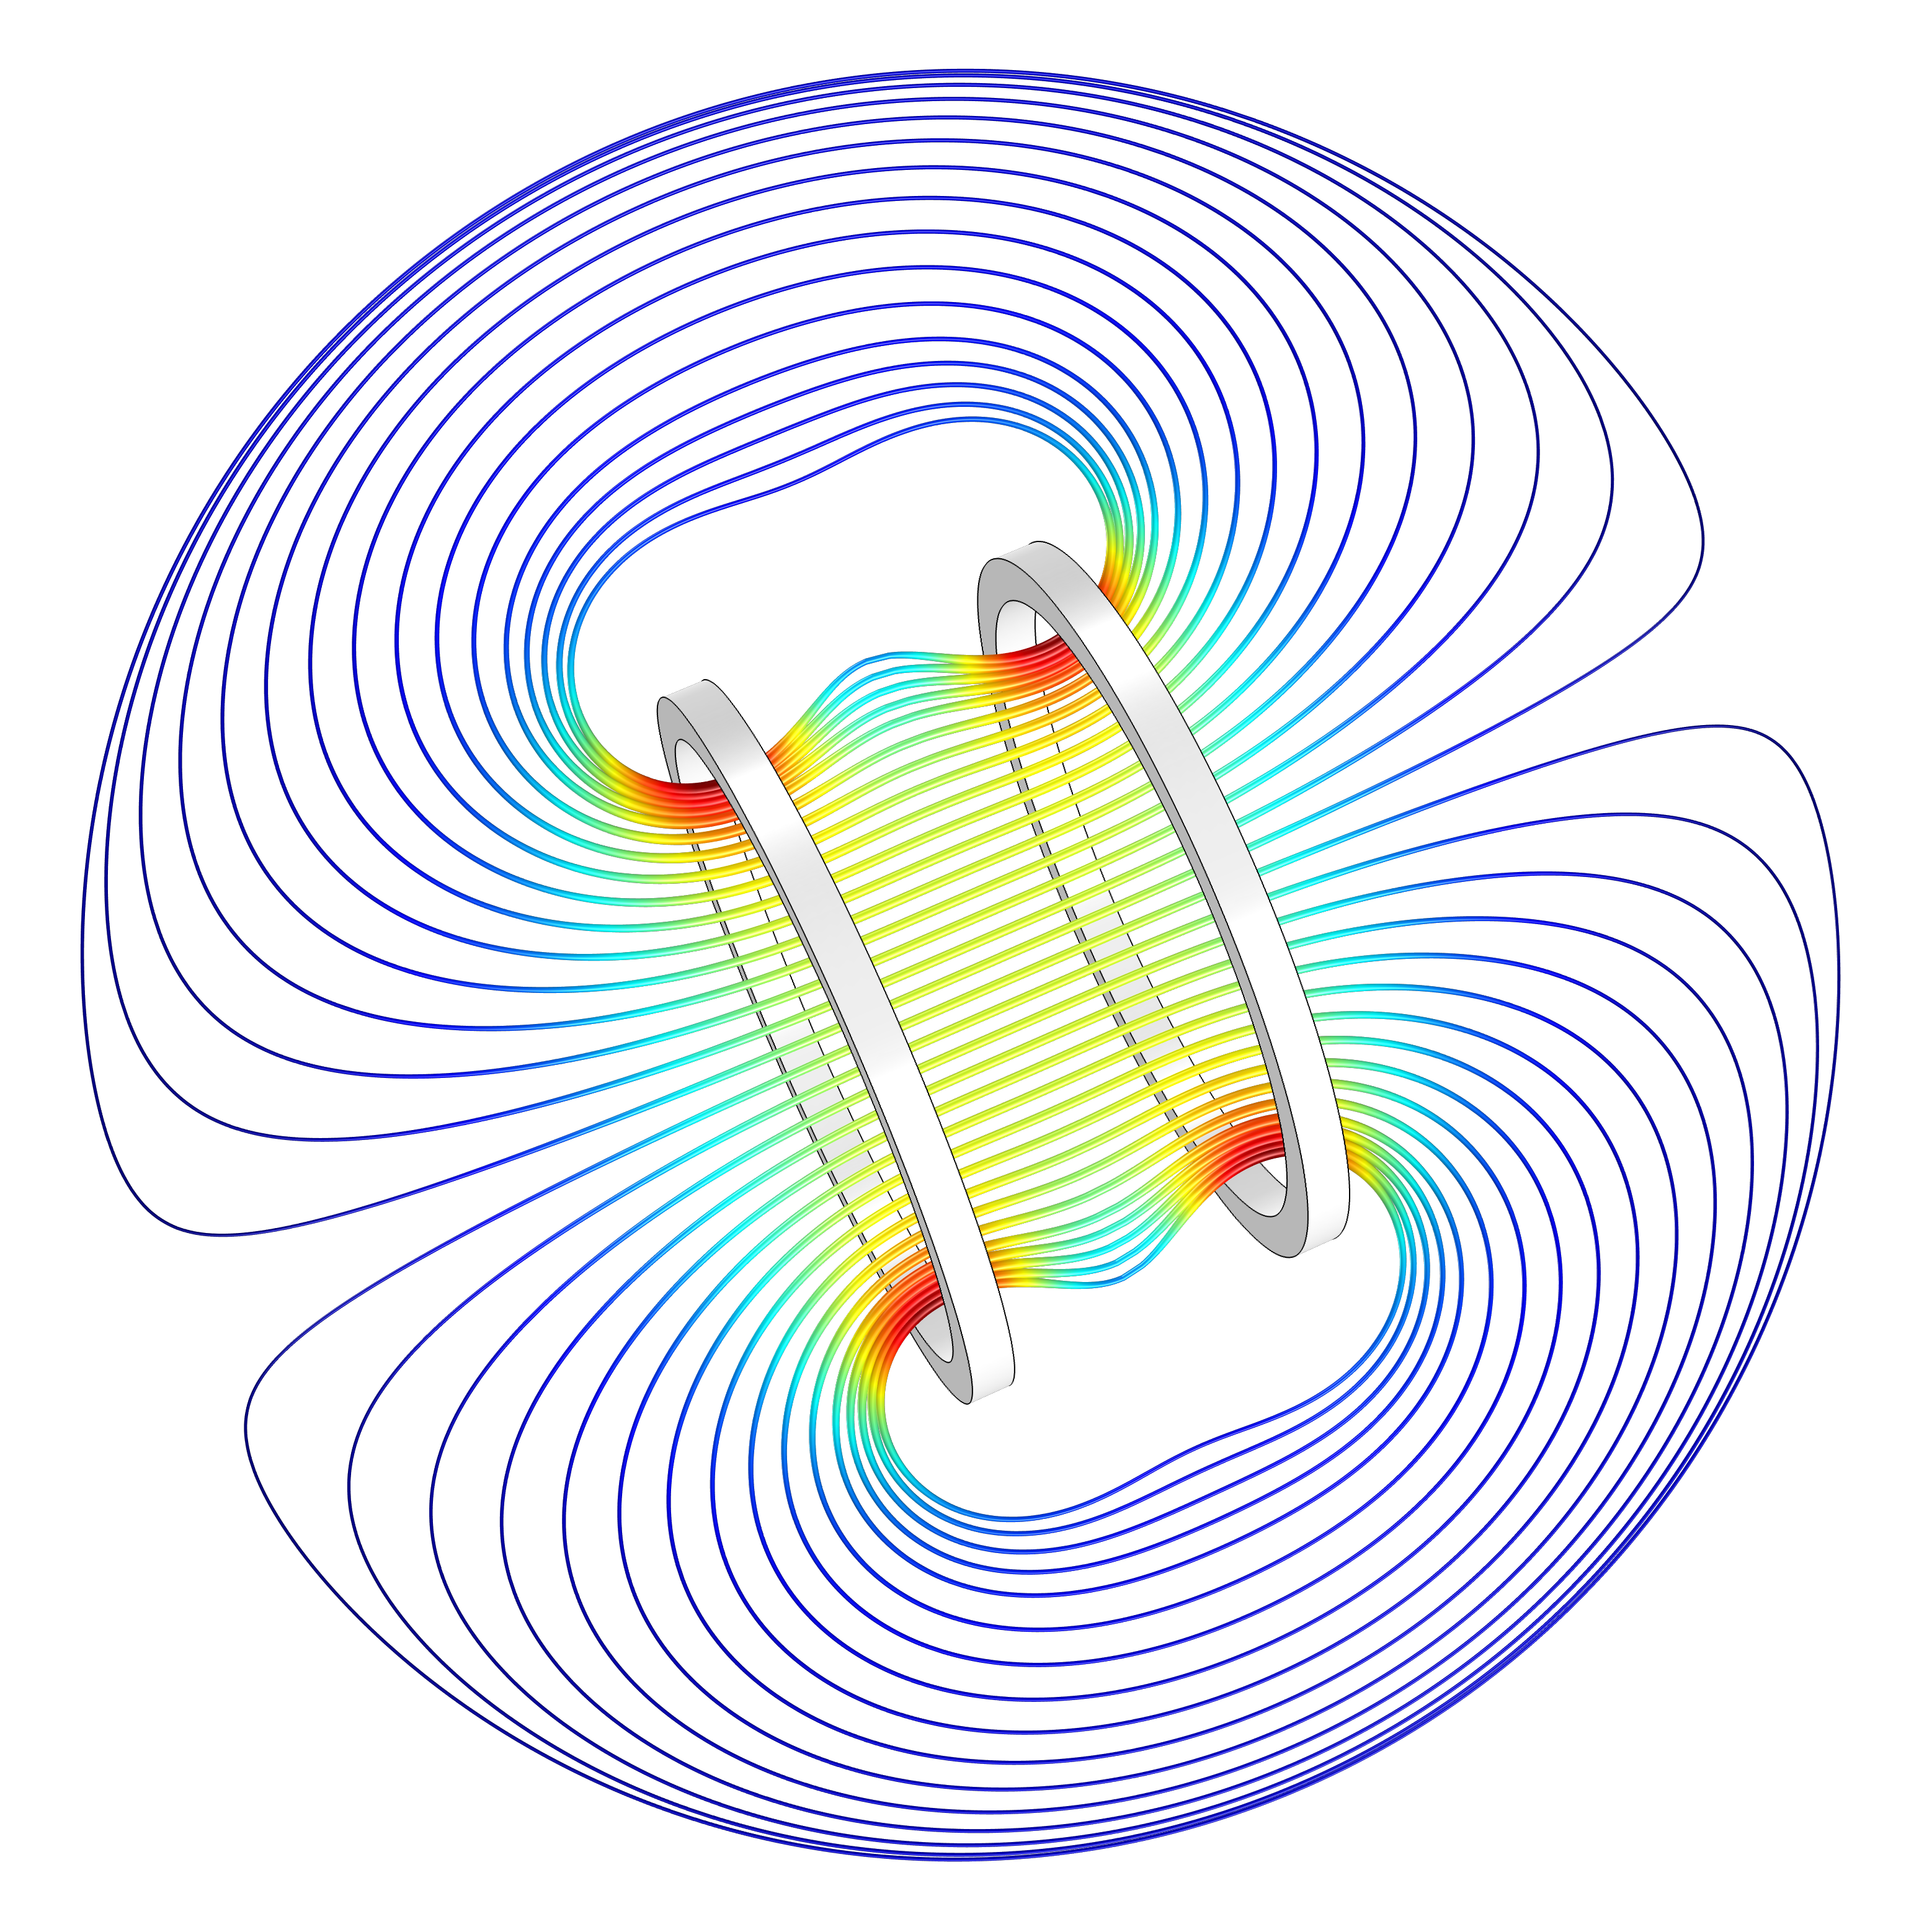
\includegraphics{BH-Diagrama}}
    \caption{Diagrama del campo generado por dos Bobinas de Helmholtz}
  \end{figure}

  En cada una de las dos partes de la práctica explicaremos más en detalle la clase de mediciones que tomaremos y las leyes que queremos demostrar.

  \newpage
  \section{Variación del campo en el eje central}

  En esta primera experiecia colocaremos las bobinas de la manera descrita a tres distancias: Igual al radio, la mitad del radio y el doble del radio. Luego moveremos el teslamómetro desde el punto central hacia los lados, siempre siguiendo el eje central. De esta manera, obtendremos 50 medidas en las que lo único que variamos es la distancia, dejando la intensidad constante.

  \subsection{Tablas de datos}

  Procedemos a exponer las tablas que obtuvimos. En ellas se representa la distancia al centro (z) en metros (m) y el campo que medimos ($B_{exp}$) en teslas (T). La incertidumbre de ambas medidas es constante, por lo que la explicitaremos aquí y no en las tablas:
  \begin{gather}
    s(B_{exp}) = 0.01mT = 10^{-5}T \\
    z = d - d_0 \qquad s(z) = \sqrt{s(d)^2 + s(d_0)^2} = \sqrt{2} \cdot s(d) = \sqrt{2} \cdot 0,001m = 0,0014m
  \end{gather}
  La intensidad también será constante y su valor e incertidumbre se fijarán en $I = 2,55 \pm 0,01 A$.

  \subsubsection{Tabla 1: Separación a=R}

  \begin{figure}[H]
    \begin{table}[H]
      \centering
      \scalebox{.71}{
      \csvreader[
        tabular=|c|c|c|,
        table head=\hline Medida & $z(m)$ & $B_{exp}(T)$ \\ \hline,
        late after last line=\\\hline,
        filter test= \ifnumless{\thecsvrow}{25},
        separator=semicolon
        ]{BH-1.csv}
        {z=\z, Bexp=\be}
        {\thecsvrow & \z & \be}} \quad
      \scalebox{.71}{
      \csvreader[
        tabular=|c|c|c|,
        table head=\hline Medida & $z(m)$ & $B_{exp}(T)$ \\ \hline,
        late after last line=\\\hline,
        separator=semicolon
        ]{BH-1b.csv}
        {z=\z, Bexp=\be}
        {\the\numexpr25+\thecsvrow\relax & \z & \be}}
    \end{table}
    \caption{Variación de B con a=R}
  \end{figure}

  Para determinar la desviación cuadrática de los datos de la tabla anterior usaremos la siguiente fórmula:
  \begin{equation}
    s = \frac{1}{N} \sqrt{\sum{\left(B_{exp} - B_{teo}\right)^2}} \label{ec:s}
  \end{equation}

  Para nuestras medidas, obtenemos $s_1 = 1,1 \cdot 10^{-5} T$.

  \vspace{1cm}

  \begin{minipage}{0.49\textwidth}
    \subsubsection{Tabla 2: Separación a=R/2}

    \begin{figure}[H]
      \begin{table}[H]
        \scalebox{.71}{
        \csvreader[
          tabular=|c|c|c|,
          table head=\hline Medida & $z(m)$ & $B_{exp}(T)$ \\ \hline,
          late after last line=\\\hline,
          filter test= \ifnumless{\thecsvrow}{25},
          separator=semicolon
          ]{BH-2.csv}
          {z=\z, Bexp=\be}
          {\thecsvrow & \z & \be}} \quad
        \scalebox{.71}{
        \csvreader[
          tabular=|c|c|c|,
          table head=\hline Medida & $z(m)$ & $B_{exp}(T)$ \\ \hline,
          late after last line=\\\hline,
          separator=semicolon
          ]{BH-2b.csv}
          {z=\z, Bexp=\be}
          {\the\numexpr25+\thecsvrow\relax & \z & \be}}
      \end{table}
      \caption{Variación de B con a=R/2}
    \end{figure}

    Calculamos la desviación típica (\ref{ec:s}) con estos datos y obtenemos $s_2 = 3,3 \cdot 10^{-5} T$.
  \end{minipage} \hfill
  \begin{minipage}{0.49\textwidth}
    \subsubsection{Tabla 3: Separación a=2R}

    \begin{figure}[H]
      \begin{table}[H]
        \scalebox{.71}{
        \csvreader[
          tabular=|c|c|c|,
          table head=\hline Medida & $z(m)$ & $B_{exp}(T)$ \\ \hline,
          late after last line=\\\hline,
          filter test= \ifnumless{\thecsvrow}{25},
          separator=semicolon
          ]{BH-3.csv}
          {z=\z, Bexp=\be}
          {\thecsvrow & \z & \be}} \quad
        \scalebox{.71}{
        \csvreader[
          tabular=|c|c|c|,
          table head=\hline Medida & $z(m)$ & $B_{exp}(T)$ \\ \hline,
          late after last line=\\\hline,
          separator=semicolon
          ]{BH-3b.csv}
          {z=\z, Bexp=\be}
          {\the\numexpr25+\thecsvrow\relax & \z & \be}}
      \end{table}
      \caption{Variación de B con a=2R}
    \end{figure}

    Calculamos la desviación típica (\ref{ec:s}) con estos datos y obtenemos $s_3 = 7,5 \cdot 10^{-5} T$.
  \end{minipage}

  \newpage
  \subsection{Campo teórico}

  Ahora debemos calcular el campo magnético teórico para poder comprarlo con los datos que obtuvimos y poder crear la gráfica que contenga a ambos.

  Utilizaremos la ecuación \ref{ec:B} y sustituiremos los valores de a=R, a=R/2 y a=2R.
  \begin{gather*}
    B1_{teo} = \frac{\mu_0 I N}{2R} \cdot \left[\frac{1}{\left(1 + \left(\frac{z - \frac{R}{2}}{R}\right)^2 \right)^{3/2}} + \frac{1}{\left(1 + \left(\frac{z + \frac{R}{2}}{R}\right)^2 \right)^{3/2}}\right] \nonumber \\
    B2_{teo} = \frac{\mu_0 I N}{2R} \cdot \left[\frac{1}{\left(1 + \left(\frac{z - \frac{R}{4}}{R}\right)^2 \right)^{3/2}} + \frac{1}{\left(1 + \left(\frac{z + \frac{R}{4}}{R}\right)^2 \right)^{3/2}}\right] \nonumber \\
    B3_{teo} = \frac{\mu_0 I N}{2R} \cdot \left[\frac{1}{\left(1 + \left(\frac{z - R}{R}\right)^2 \right)^{3/2}} + \frac{1}{\left(1 + \left(\frac{z + R}{R}\right)^2 \right)^{3/2}}\right] \nonumber
  \end{gather*}

  Ahora, con estas ecuaciones, sustituiremos el valor del radio R=0.20m, la permeabilidad magnética $\mu_0 = 4 \pi 10^{-7}$, el número de espiras N=154 y la intensidad I=2,55A. Esto nos dará una fórmula general para calcular los valores de B sustituyendo las distancias z correspondientes. Presentamos los resultados corresponiendtes en las siguientes tablas:

  \textit{(En la siguiente página por comodidad de representación.)}

  \begin{figure}[H]
    \begin{table}[H]
      \centering
      \scalebox{.7}{
      \csvreader[
        tabular=|c|,
        table head=\hline Medida \\ \hline,
        late after last line=\\\hline,
        separator=semicolon
        ]{BH-1.csv}
        {}
        {\thecsvrow}} \quad
      \scalebox{.7}{
      \csvreader[
        tabular=|c|c|c|,
        table head=\hline $z1(m)$ & $B1_{exp}(T)$ & $B1_{teo}(T)$ \\ \hline,
        late after last line=\\\hline,
        separator=semicolon
        ]{BH-1.csv}
        {z=\z, Bteo=\bt, Bexp=\be}
        {\z & \be & \bt}} \quad
      \scalebox{.7}{
      \csvreader[
        tabular=|c|c|c|,
        table head=\hline $z2(m)$ & $B2_{exp}(T)$ & $B2_{teo}(T)$ \\ \hline,
        late after last line=\\\hline,
        separator=semicolon
        ]{BH-2.csv}
        {z=\z, Bteo=\bt, Bexp=\be}
        {\z & \be & \bt}} \quad
      \scalebox{.7}{
      \csvreader[
        tabular=|c|c|c|,
        table head=\hline $z3(m)$ & $B3_{exp}(T)$ & $B3_{teo}(T)$ \\ \hline,
        late after last line=\\\hline,
        separator=semicolon
        ]{BH-3.csv}
        {z=\z, Bteo=\bt, Bexp=\be}
        {\z & \be & \bt}} \quad
    \end{table}
    \caption{Campo magnético experimental frente a teórico para a=R, a=R/2 y a=2R}
  \end{figure}

  \subsection{Representación gráfica}

  Finalmente, teniendo los datos del campo magnético experimental y sabiendo calcular los del campo magnético teórico, representaremos ambos para poder compararlos. Cabe destacar que no utilizaremos los datos $B_{teo}$ de la tabla anterior, si no que computaremos la fórmula directamente en python para obtener una curva más suave. La tabla anterior era simplemente una demostración de cómo calcular el campo teórico.

  Primero procesaremos los datos en \code{python}, y para ello haremos uso de la librería \code{pandas}, que nos permite importar directamente archivos .csv, el mismo formato que usamos para representar las tablas de \LaTeX.

  \begin{python}
    import pandas as pd

    #Constantes
    pm = 4 * np.pi * 10**(-7); i = 2.55; n = 154; r = 0.2

    #Leer datos
    d1 = pd.read_csv("BH-1.csv", sep=';', decimal=',')
    z1 = d1["z"]; Be1 = d1["Bexp"] #Similarmente para las otras tablas
  \end{python}

  El siguiente paso es calcular las curvas teóricas, para las que utilizaremos una función por comodidad. Para ellas definiremos $z \subset [-0,450, 0,450]$ con medidas cada 0,02m, ya que nos dará una representación simétrica y que contenga todas las medidas experimentales.

  \begin{python}
    #Calculo campo magnetico
    B = lambda pm, i, n, r, a, z: ((pm * i * n) / (2 * r)) *
        ((1 / (1 + ((z - (a/2)) / (r))**2)**(3/2)) +
        (1 / (1 + ((z + (a/2)) / (r))**2)**(3/2)))

    #Curvas teoricas
    z = np.linspace(-0.450, 0.450, 450)
    Bt1 = B(pm, i, n, r, r, z)
    Bt2 = B(pm, i, n, r, r/2, z)
    Bt3 = B(pm, i, n, r, 2*r, z)
  \end{python}

  Por fin estamos listos para representar las gráficas, lo que haremos con ayuda de \code{matplotlib}. Las exportaremos utilizando un formato .pgf que \LaTeX puede leer de mandera vectorial.

  \begin{python}
    import matplotlib.pyplot as plt

    #Graficas experimentales (puntos)
    plt.scatter(z1,Be1);plt.scatter(z2,Be2);plt.scatter(z3,Be3)
    #Graficas teoricas (curvas)
    plt.plot(z,Bt1); plt.plot(z,Bt2); plt.plot(z,Bt2)
  \end{python}

  Además de nuestro programa original, utilizaremos un complemento común para todas las memorias que define el estilo de las gráficas y configura \code{matplotlib} para exportar .pgf y utilizar nuestra paleta de colores.

  Al ejecutar el código, obtenemos la siguiente gráfica:

  \begin{figure}[H]
    %\centering
    \hspace{2.5em} %% Creator: Matplotlib, PGF backend
%%
%% To include the figure in your LaTeX document, write
%%   \input{<filename>.pgf}
%%
%% Make sure the required packages are loaded in your preamble
%%   \usepackage{pgf}
%%
%% and, on pdftex
%%   \usepackage[utf8]{inputenc}\DeclareUnicodeCharacter{2212}{-}
%%
%% or, on luatex and xetex
%%   \usepackage{unicode-math}
%%
%% Figures using additional raster images can only be included by \input if
%% they are in the same directory as the main LaTeX file. For loading figures
%% from other directories you can use the `import` package
%%   \usepackage{import}
%%
%% and then include the figures with
%%   \import{<path to file>}{<filename>.pgf}
%%
%% Matplotlib used the following preamble
%%
\begingroup%
\makeatletter%
\begin{pgfpicture}%
\pgfpathrectangle{\pgfpointorigin}{\pgfqpoint{4.989160in}{3.257623in}}%
\pgfusepath{use as bounding box, clip}%
\begin{pgfscope}%
\pgfsetbuttcap%
\pgfsetmiterjoin%
\definecolor{currentfill}{rgb}{1.000000,1.000000,1.000000}%
\pgfsetfillcolor{currentfill}%
\pgfsetlinewidth{0.000000pt}%
\definecolor{currentstroke}{rgb}{1.000000,1.000000,1.000000}%
\pgfsetstrokecolor{currentstroke}%
\pgfsetdash{}{0pt}%
\pgfpathmoveto{\pgfqpoint{0.000000in}{-0.000000in}}%
\pgfpathlineto{\pgfqpoint{4.989160in}{-0.000000in}}%
\pgfpathlineto{\pgfqpoint{4.989160in}{3.257623in}}%
\pgfpathlineto{\pgfqpoint{0.000000in}{3.257623in}}%
\pgfpathclose%
\pgfusepath{fill}%
\end{pgfscope}%
\begin{pgfscope}%
\pgfsetbuttcap%
\pgfsetmiterjoin%
\definecolor{currentfill}{rgb}{1.000000,1.000000,1.000000}%
\pgfsetfillcolor{currentfill}%
\pgfsetlinewidth{0.000000pt}%
\definecolor{currentstroke}{rgb}{0.000000,0.000000,0.000000}%
\pgfsetstrokecolor{currentstroke}%
\pgfsetstrokeopacity{0.000000}%
\pgfsetdash{}{0pt}%
\pgfpathmoveto{\pgfqpoint{1.014160in}{0.515123in}}%
\pgfpathlineto{\pgfqpoint{4.889160in}{0.515123in}}%
\pgfpathlineto{\pgfqpoint{4.889160in}{3.157623in}}%
\pgfpathlineto{\pgfqpoint{1.014160in}{3.157623in}}%
\pgfpathclose%
\pgfusepath{fill}%
\end{pgfscope}%
\begin{pgfscope}%
\pgfpathrectangle{\pgfqpoint{1.014160in}{0.515123in}}{\pgfqpoint{3.875000in}{2.642500in}}%
\pgfusepath{clip}%
\pgfsetbuttcap%
\pgfsetroundjoin%
\definecolor{currentfill}{rgb}{0.254902,0.411765,0.882353}%
\pgfsetfillcolor{currentfill}%
\pgfsetlinewidth{0.501875pt}%
\definecolor{currentstroke}{rgb}{0.000000,0.000000,0.000000}%
\pgfsetstrokecolor{currentstroke}%
\pgfsetdash{}{0pt}%
\pgfsys@defobject{currentmarker}{\pgfqpoint{-0.041667in}{-0.041667in}}{\pgfqpoint{0.041667in}{0.041667in}}{%
\pgfpathmoveto{\pgfqpoint{0.000000in}{-0.041667in}}%
\pgfpathcurveto{\pgfqpoint{0.011050in}{-0.041667in}}{\pgfqpoint{0.021649in}{-0.037276in}}{\pgfqpoint{0.029463in}{-0.029463in}}%
\pgfpathcurveto{\pgfqpoint{0.037276in}{-0.021649in}}{\pgfqpoint{0.041667in}{-0.011050in}}{\pgfqpoint{0.041667in}{0.000000in}}%
\pgfpathcurveto{\pgfqpoint{0.041667in}{0.011050in}}{\pgfqpoint{0.037276in}{0.021649in}}{\pgfqpoint{0.029463in}{0.029463in}}%
\pgfpathcurveto{\pgfqpoint{0.021649in}{0.037276in}}{\pgfqpoint{0.011050in}{0.041667in}}{\pgfqpoint{0.000000in}{0.041667in}}%
\pgfpathcurveto{\pgfqpoint{-0.011050in}{0.041667in}}{\pgfqpoint{-0.021649in}{0.037276in}}{\pgfqpoint{-0.029463in}{0.029463in}}%
\pgfpathcurveto{\pgfqpoint{-0.037276in}{0.021649in}}{\pgfqpoint{-0.041667in}{0.011050in}}{\pgfqpoint{-0.041667in}{0.000000in}}%
\pgfpathcurveto{\pgfqpoint{-0.041667in}{-0.011050in}}{\pgfqpoint{-0.037276in}{-0.021649in}}{\pgfqpoint{-0.029463in}{-0.029463in}}%
\pgfpathcurveto{\pgfqpoint{-0.021649in}{-0.037276in}}{\pgfqpoint{-0.011050in}{-0.041667in}}{\pgfqpoint{0.000000in}{-0.041667in}}%
\pgfpathclose%
\pgfusepath{stroke,fill}%
}%
\begin{pgfscope}%
\pgfsys@transformshift{3.519211in}{2.121495in}%
\pgfsys@useobject{currentmarker}{}%
\end{pgfscope}%
\begin{pgfscope}%
\pgfsys@transformshift{3.480070in}{2.167708in}%
\pgfsys@useobject{currentmarker}{}%
\end{pgfscope}%
\begin{pgfscope}%
\pgfsys@transformshift{3.440928in}{2.225473in}%
\pgfsys@useobject{currentmarker}{}%
\end{pgfscope}%
\begin{pgfscope}%
\pgfsys@transformshift{3.401787in}{2.260133in}%
\pgfsys@useobject{currentmarker}{}%
\end{pgfscope}%
\begin{pgfscope}%
\pgfsys@transformshift{3.362645in}{2.306345in}%
\pgfsys@useobject{currentmarker}{}%
\end{pgfscope}%
\begin{pgfscope}%
\pgfsys@transformshift{3.323504in}{2.352558in}%
\pgfsys@useobject{currentmarker}{}%
\end{pgfscope}%
\begin{pgfscope}%
\pgfsys@transformshift{3.284363in}{2.375664in}%
\pgfsys@useobject{currentmarker}{}%
\end{pgfscope}%
\begin{pgfscope}%
\pgfsys@transformshift{3.245221in}{2.398770in}%
\pgfsys@useobject{currentmarker}{}%
\end{pgfscope}%
\begin{pgfscope}%
\pgfsys@transformshift{3.206080in}{2.410323in}%
\pgfsys@useobject{currentmarker}{}%
\end{pgfscope}%
\begin{pgfscope}%
\pgfsys@transformshift{3.166938in}{2.398770in}%
\pgfsys@useobject{currentmarker}{}%
\end{pgfscope}%
\begin{pgfscope}%
\pgfsys@transformshift{3.127797in}{2.410323in}%
\pgfsys@useobject{currentmarker}{}%
\end{pgfscope}%
\begin{pgfscope}%
\pgfsys@transformshift{3.088655in}{2.410323in}%
\pgfsys@useobject{currentmarker}{}%
\end{pgfscope}%
\begin{pgfscope}%
\pgfsys@transformshift{3.049514in}{2.398770in}%
\pgfsys@useobject{currentmarker}{}%
\end{pgfscope}%
\begin{pgfscope}%
\pgfsys@transformshift{3.010373in}{2.410323in}%
\pgfsys@useobject{currentmarker}{}%
\end{pgfscope}%
\begin{pgfscope}%
\pgfsys@transformshift{2.971231in}{2.398770in}%
\pgfsys@useobject{currentmarker}{}%
\end{pgfscope}%
\begin{pgfscope}%
\pgfsys@transformshift{2.951660in}{2.398770in}%
\pgfsys@useobject{currentmarker}{}%
\end{pgfscope}%
\begin{pgfscope}%
\pgfsys@transformshift{2.912519in}{2.387217in}%
\pgfsys@useobject{currentmarker}{}%
\end{pgfscope}%
\begin{pgfscope}%
\pgfsys@transformshift{2.873378in}{2.387217in}%
\pgfsys@useobject{currentmarker}{}%
\end{pgfscope}%
\begin{pgfscope}%
\pgfsys@transformshift{2.834236in}{2.387217in}%
\pgfsys@useobject{currentmarker}{}%
\end{pgfscope}%
\begin{pgfscope}%
\pgfsys@transformshift{2.795095in}{2.375664in}%
\pgfsys@useobject{currentmarker}{}%
\end{pgfscope}%
\begin{pgfscope}%
\pgfsys@transformshift{2.755953in}{2.375664in}%
\pgfsys@useobject{currentmarker}{}%
\end{pgfscope}%
\begin{pgfscope}%
\pgfsys@transformshift{2.716812in}{2.364111in}%
\pgfsys@useobject{currentmarker}{}%
\end{pgfscope}%
\begin{pgfscope}%
\pgfsys@transformshift{2.677671in}{2.352558in}%
\pgfsys@useobject{currentmarker}{}%
\end{pgfscope}%
\begin{pgfscope}%
\pgfsys@transformshift{2.638529in}{2.329451in}%
\pgfsys@useobject{currentmarker}{}%
\end{pgfscope}%
\begin{pgfscope}%
\pgfsys@transformshift{2.599388in}{2.306345in}%
\pgfsys@useobject{currentmarker}{}%
\end{pgfscope}%
\begin{pgfscope}%
\pgfsys@transformshift{2.560246in}{2.283239in}%
\pgfsys@useobject{currentmarker}{}%
\end{pgfscope}%
\begin{pgfscope}%
\pgfsys@transformshift{2.521105in}{2.225473in}%
\pgfsys@useobject{currentmarker}{}%
\end{pgfscope}%
\begin{pgfscope}%
\pgfsys@transformshift{2.481964in}{2.179261in}%
\pgfsys@useobject{currentmarker}{}%
\end{pgfscope}%
\begin{pgfscope}%
\pgfsys@transformshift{2.442822in}{2.109942in}%
\pgfsys@useobject{currentmarker}{}%
\end{pgfscope}%
\begin{pgfscope}%
\pgfsys@transformshift{2.403681in}{2.052177in}%
\pgfsys@useobject{currentmarker}{}%
\end{pgfscope}%
\begin{pgfscope}%
\pgfsys@transformshift{2.364539in}{1.982858in}%
\pgfsys@useobject{currentmarker}{}%
\end{pgfscope}%
\begin{pgfscope}%
\pgfsys@transformshift{2.325398in}{1.913539in}%
\pgfsys@useobject{currentmarker}{}%
\end{pgfscope}%
\begin{pgfscope}%
\pgfsys@transformshift{2.286256in}{1.832667in}%
\pgfsys@useobject{currentmarker}{}%
\end{pgfscope}%
\begin{pgfscope}%
\pgfsys@transformshift{2.247115in}{1.751795in}%
\pgfsys@useobject{currentmarker}{}%
\end{pgfscope}%
\begin{pgfscope}%
\pgfsys@transformshift{2.207974in}{1.670924in}%
\pgfsys@useobject{currentmarker}{}%
\end{pgfscope}%
\begin{pgfscope}%
\pgfsys@transformshift{2.168832in}{1.601605in}%
\pgfsys@useobject{currentmarker}{}%
\end{pgfscope}%
\begin{pgfscope}%
\pgfsys@transformshift{2.129691in}{1.532286in}%
\pgfsys@useobject{currentmarker}{}%
\end{pgfscope}%
\begin{pgfscope}%
\pgfsys@transformshift{2.090549in}{1.462967in}%
\pgfsys@useobject{currentmarker}{}%
\end{pgfscope}%
\begin{pgfscope}%
\pgfsys@transformshift{2.051408in}{1.382096in}%
\pgfsys@useobject{currentmarker}{}%
\end{pgfscope}%
\begin{pgfscope}%
\pgfsys@transformshift{2.012267in}{1.324330in}%
\pgfsys@useobject{currentmarker}{}%
\end{pgfscope}%
\begin{pgfscope}%
\pgfsys@transformshift{1.973125in}{1.208799in}%
\pgfsys@useobject{currentmarker}{}%
\end{pgfscope}%
\begin{pgfscope}%
\pgfsys@transformshift{1.933984in}{1.151033in}%
\pgfsys@useobject{currentmarker}{}%
\end{pgfscope}%
\begin{pgfscope}%
\pgfsys@transformshift{1.894842in}{1.093268in}%
\pgfsys@useobject{currentmarker}{}%
\end{pgfscope}%
\begin{pgfscope}%
\pgfsys@transformshift{1.855701in}{1.035502in}%
\pgfsys@useobject{currentmarker}{}%
\end{pgfscope}%
\begin{pgfscope}%
\pgfsys@transformshift{1.816559in}{0.989289in}%
\pgfsys@useobject{currentmarker}{}%
\end{pgfscope}%
\begin{pgfscope}%
\pgfsys@transformshift{1.777418in}{0.954630in}%
\pgfsys@useobject{currentmarker}{}%
\end{pgfscope}%
\begin{pgfscope}%
\pgfsys@transformshift{1.738277in}{0.919971in}%
\pgfsys@useobject{currentmarker}{}%
\end{pgfscope}%
\begin{pgfscope}%
\pgfsys@transformshift{1.699135in}{0.885311in}%
\pgfsys@useobject{currentmarker}{}%
\end{pgfscope}%
\begin{pgfscope}%
\pgfsys@transformshift{1.659994in}{0.862205in}%
\pgfsys@useobject{currentmarker}{}%
\end{pgfscope}%
\begin{pgfscope}%
\pgfsys@transformshift{1.620852in}{0.827546in}%
\pgfsys@useobject{currentmarker}{}%
\end{pgfscope}%
\end{pgfscope}%
\begin{pgfscope}%
\pgfpathrectangle{\pgfqpoint{1.014160in}{0.515123in}}{\pgfqpoint{3.875000in}{2.642500in}}%
\pgfusepath{clip}%
\pgfsetbuttcap%
\pgfsetroundjoin%
\definecolor{currentfill}{rgb}{0.235294,0.701961,0.443137}%
\pgfsetfillcolor{currentfill}%
\pgfsetlinewidth{0.501875pt}%
\definecolor{currentstroke}{rgb}{0.000000,0.000000,0.000000}%
\pgfsetstrokecolor{currentstroke}%
\pgfsetdash{}{0pt}%
\pgfsys@defobject{currentmarker}{\pgfqpoint{-0.041667in}{-0.041667in}}{\pgfqpoint{0.041667in}{0.041667in}}{%
\pgfpathmoveto{\pgfqpoint{0.000000in}{-0.041667in}}%
\pgfpathcurveto{\pgfqpoint{0.011050in}{-0.041667in}}{\pgfqpoint{0.021649in}{-0.037276in}}{\pgfqpoint{0.029463in}{-0.029463in}}%
\pgfpathcurveto{\pgfqpoint{0.037276in}{-0.021649in}}{\pgfqpoint{0.041667in}{-0.011050in}}{\pgfqpoint{0.041667in}{0.000000in}}%
\pgfpathcurveto{\pgfqpoint{0.041667in}{0.011050in}}{\pgfqpoint{0.037276in}{0.021649in}}{\pgfqpoint{0.029463in}{0.029463in}}%
\pgfpathcurveto{\pgfqpoint{0.021649in}{0.037276in}}{\pgfqpoint{0.011050in}{0.041667in}}{\pgfqpoint{0.000000in}{0.041667in}}%
\pgfpathcurveto{\pgfqpoint{-0.011050in}{0.041667in}}{\pgfqpoint{-0.021649in}{0.037276in}}{\pgfqpoint{-0.029463in}{0.029463in}}%
\pgfpathcurveto{\pgfqpoint{-0.037276in}{0.021649in}}{\pgfqpoint{-0.041667in}{0.011050in}}{\pgfqpoint{-0.041667in}{0.000000in}}%
\pgfpathcurveto{\pgfqpoint{-0.041667in}{-0.011050in}}{\pgfqpoint{-0.037276in}{-0.021649in}}{\pgfqpoint{-0.029463in}{-0.029463in}}%
\pgfpathcurveto{\pgfqpoint{-0.021649in}{-0.037276in}}{\pgfqpoint{-0.011050in}{-0.041667in}}{\pgfqpoint{0.000000in}{-0.041667in}}%
\pgfpathclose%
\pgfusepath{stroke,fill}%
}%
\begin{pgfscope}%
\pgfsys@transformshift{3.636635in}{1.705583in}%
\pgfsys@useobject{currentmarker}{}%
\end{pgfscope}%
\begin{pgfscope}%
\pgfsys@transformshift{3.597494in}{1.798008in}%
\pgfsys@useobject{currentmarker}{}%
\end{pgfscope}%
\begin{pgfscope}%
\pgfsys@transformshift{3.558352in}{1.878880in}%
\pgfsys@useobject{currentmarker}{}%
\end{pgfscope}%
\begin{pgfscope}%
\pgfsys@transformshift{3.519211in}{1.982858in}%
\pgfsys@useobject{currentmarker}{}%
\end{pgfscope}%
\begin{pgfscope}%
\pgfsys@transformshift{3.480070in}{2.086836in}%
\pgfsys@useobject{currentmarker}{}%
\end{pgfscope}%
\begin{pgfscope}%
\pgfsys@transformshift{3.440928in}{2.179261in}%
\pgfsys@useobject{currentmarker}{}%
\end{pgfscope}%
\begin{pgfscope}%
\pgfsys@transformshift{3.401787in}{2.283239in}%
\pgfsys@useobject{currentmarker}{}%
\end{pgfscope}%
\begin{pgfscope}%
\pgfsys@transformshift{3.362645in}{2.375664in}%
\pgfsys@useobject{currentmarker}{}%
\end{pgfscope}%
\begin{pgfscope}%
\pgfsys@transformshift{3.323504in}{2.479642in}%
\pgfsys@useobject{currentmarker}{}%
\end{pgfscope}%
\begin{pgfscope}%
\pgfsys@transformshift{3.284363in}{2.572067in}%
\pgfsys@useobject{currentmarker}{}%
\end{pgfscope}%
\begin{pgfscope}%
\pgfsys@transformshift{3.245221in}{2.652939in}%
\pgfsys@useobject{currentmarker}{}%
\end{pgfscope}%
\begin{pgfscope}%
\pgfsys@transformshift{3.206080in}{2.745364in}%
\pgfsys@useobject{currentmarker}{}%
\end{pgfscope}%
\begin{pgfscope}%
\pgfsys@transformshift{3.166938in}{2.803129in}%
\pgfsys@useobject{currentmarker}{}%
\end{pgfscope}%
\begin{pgfscope}%
\pgfsys@transformshift{3.127797in}{2.837789in}%
\pgfsys@useobject{currentmarker}{}%
\end{pgfscope}%
\begin{pgfscope}%
\pgfsys@transformshift{3.088655in}{2.895554in}%
\pgfsys@useobject{currentmarker}{}%
\end{pgfscope}%
\begin{pgfscope}%
\pgfsys@transformshift{3.049514in}{2.930214in}%
\pgfsys@useobject{currentmarker}{}%
\end{pgfscope}%
\begin{pgfscope}%
\pgfsys@transformshift{3.010373in}{2.941767in}%
\pgfsys@useobject{currentmarker}{}%
\end{pgfscope}%
\begin{pgfscope}%
\pgfsys@transformshift{2.971231in}{2.941767in}%
\pgfsys@useobject{currentmarker}{}%
\end{pgfscope}%
\begin{pgfscope}%
\pgfsys@transformshift{2.951660in}{2.941767in}%
\pgfsys@useobject{currentmarker}{}%
\end{pgfscope}%
\begin{pgfscope}%
\pgfsys@transformshift{2.912519in}{2.930214in}%
\pgfsys@useobject{currentmarker}{}%
\end{pgfscope}%
\begin{pgfscope}%
\pgfsys@transformshift{2.873378in}{2.895554in}%
\pgfsys@useobject{currentmarker}{}%
\end{pgfscope}%
\begin{pgfscope}%
\pgfsys@transformshift{2.834236in}{2.860895in}%
\pgfsys@useobject{currentmarker}{}%
\end{pgfscope}%
\begin{pgfscope}%
\pgfsys@transformshift{2.795095in}{2.803129in}%
\pgfsys@useobject{currentmarker}{}%
\end{pgfscope}%
\begin{pgfscope}%
\pgfsys@transformshift{2.755953in}{2.745364in}%
\pgfsys@useobject{currentmarker}{}%
\end{pgfscope}%
\begin{pgfscope}%
\pgfsys@transformshift{2.716812in}{2.676045in}%
\pgfsys@useobject{currentmarker}{}%
\end{pgfscope}%
\begin{pgfscope}%
\pgfsys@transformshift{2.677671in}{2.583620in}%
\pgfsys@useobject{currentmarker}{}%
\end{pgfscope}%
\begin{pgfscope}%
\pgfsys@transformshift{2.638529in}{2.491195in}%
\pgfsys@useobject{currentmarker}{}%
\end{pgfscope}%
\begin{pgfscope}%
\pgfsys@transformshift{2.599388in}{2.387217in}%
\pgfsys@useobject{currentmarker}{}%
\end{pgfscope}%
\begin{pgfscope}%
\pgfsys@transformshift{2.560246in}{2.306345in}%
\pgfsys@useobject{currentmarker}{}%
\end{pgfscope}%
\begin{pgfscope}%
\pgfsys@transformshift{2.521105in}{2.213920in}%
\pgfsys@useobject{currentmarker}{}%
\end{pgfscope}%
\begin{pgfscope}%
\pgfsys@transformshift{2.481964in}{2.109942in}%
\pgfsys@useobject{currentmarker}{}%
\end{pgfscope}%
\begin{pgfscope}%
\pgfsys@transformshift{2.442822in}{2.005964in}%
\pgfsys@useobject{currentmarker}{}%
\end{pgfscope}%
\begin{pgfscope}%
\pgfsys@transformshift{2.403681in}{1.901986in}%
\pgfsys@useobject{currentmarker}{}%
\end{pgfscope}%
\begin{pgfscope}%
\pgfsys@transformshift{2.364539in}{1.821114in}%
\pgfsys@useobject{currentmarker}{}%
\end{pgfscope}%
\begin{pgfscope}%
\pgfsys@transformshift{2.325398in}{1.717136in}%
\pgfsys@useobject{currentmarker}{}%
\end{pgfscope}%
\begin{pgfscope}%
\pgfsys@transformshift{2.286256in}{1.636264in}%
\pgfsys@useobject{currentmarker}{}%
\end{pgfscope}%
\begin{pgfscope}%
\pgfsys@transformshift{2.247115in}{1.543839in}%
\pgfsys@useobject{currentmarker}{}%
\end{pgfscope}%
\begin{pgfscope}%
\pgfsys@transformshift{2.207974in}{1.474521in}%
\pgfsys@useobject{currentmarker}{}%
\end{pgfscope}%
\begin{pgfscope}%
\pgfsys@transformshift{2.168832in}{1.393649in}%
\pgfsys@useobject{currentmarker}{}%
\end{pgfscope}%
\begin{pgfscope}%
\pgfsys@transformshift{2.129691in}{1.312777in}%
\pgfsys@useobject{currentmarker}{}%
\end{pgfscope}%
\begin{pgfscope}%
\pgfsys@transformshift{2.090549in}{1.255011in}%
\pgfsys@useobject{currentmarker}{}%
\end{pgfscope}%
\begin{pgfscope}%
\pgfsys@transformshift{2.051408in}{1.197246in}%
\pgfsys@useobject{currentmarker}{}%
\end{pgfscope}%
\begin{pgfscope}%
\pgfsys@transformshift{2.012267in}{1.139480in}%
\pgfsys@useobject{currentmarker}{}%
\end{pgfscope}%
\begin{pgfscope}%
\pgfsys@transformshift{1.973125in}{1.081714in}%
\pgfsys@useobject{currentmarker}{}%
\end{pgfscope}%
\begin{pgfscope}%
\pgfsys@transformshift{1.933984in}{1.035502in}%
\pgfsys@useobject{currentmarker}{}%
\end{pgfscope}%
\begin{pgfscope}%
\pgfsys@transformshift{1.894842in}{1.000843in}%
\pgfsys@useobject{currentmarker}{}%
\end{pgfscope}%
\begin{pgfscope}%
\pgfsys@transformshift{1.855701in}{0.954630in}%
\pgfsys@useobject{currentmarker}{}%
\end{pgfscope}%
\begin{pgfscope}%
\pgfsys@transformshift{1.816559in}{0.919971in}%
\pgfsys@useobject{currentmarker}{}%
\end{pgfscope}%
\begin{pgfscope}%
\pgfsys@transformshift{1.777418in}{0.896864in}%
\pgfsys@useobject{currentmarker}{}%
\end{pgfscope}%
\begin{pgfscope}%
\pgfsys@transformshift{1.738277in}{0.873758in}%
\pgfsys@useobject{currentmarker}{}%
\end{pgfscope}%
\end{pgfscope}%
\begin{pgfscope}%
\pgfpathrectangle{\pgfqpoint{1.014160in}{0.515123in}}{\pgfqpoint{3.875000in}{2.642500in}}%
\pgfusepath{clip}%
\pgfsetbuttcap%
\pgfsetroundjoin%
\definecolor{currentfill}{rgb}{1.000000,0.388235,0.278431}%
\pgfsetfillcolor{currentfill}%
\pgfsetlinewidth{0.501875pt}%
\definecolor{currentstroke}{rgb}{0.000000,0.000000,0.000000}%
\pgfsetstrokecolor{currentstroke}%
\pgfsetdash{}{0pt}%
\pgfsys@defobject{currentmarker}{\pgfqpoint{-0.041667in}{-0.041667in}}{\pgfqpoint{0.041667in}{0.041667in}}{%
\pgfpathmoveto{\pgfqpoint{0.000000in}{-0.041667in}}%
\pgfpathcurveto{\pgfqpoint{0.011050in}{-0.041667in}}{\pgfqpoint{0.021649in}{-0.037276in}}{\pgfqpoint{0.029463in}{-0.029463in}}%
\pgfpathcurveto{\pgfqpoint{0.037276in}{-0.021649in}}{\pgfqpoint{0.041667in}{-0.011050in}}{\pgfqpoint{0.041667in}{0.000000in}}%
\pgfpathcurveto{\pgfqpoint{0.041667in}{0.011050in}}{\pgfqpoint{0.037276in}{0.021649in}}{\pgfqpoint{0.029463in}{0.029463in}}%
\pgfpathcurveto{\pgfqpoint{0.021649in}{0.037276in}}{\pgfqpoint{0.011050in}{0.041667in}}{\pgfqpoint{0.000000in}{0.041667in}}%
\pgfpathcurveto{\pgfqpoint{-0.011050in}{0.041667in}}{\pgfqpoint{-0.021649in}{0.037276in}}{\pgfqpoint{-0.029463in}{0.029463in}}%
\pgfpathcurveto{\pgfqpoint{-0.037276in}{0.021649in}}{\pgfqpoint{-0.041667in}{0.011050in}}{\pgfqpoint{-0.041667in}{0.000000in}}%
\pgfpathcurveto{\pgfqpoint{-0.041667in}{-0.011050in}}{\pgfqpoint{-0.037276in}{-0.021649in}}{\pgfqpoint{-0.029463in}{-0.029463in}}%
\pgfpathcurveto{\pgfqpoint{-0.021649in}{-0.037276in}}{\pgfqpoint{-0.011050in}{-0.041667in}}{\pgfqpoint{0.000000in}{-0.041667in}}%
\pgfpathclose%
\pgfusepath{stroke,fill}%
}%
\begin{pgfscope}%
\pgfsys@transformshift{3.088655in}{1.416755in}%
\pgfsys@useobject{currentmarker}{}%
\end{pgfscope}%
\begin{pgfscope}%
\pgfsys@transformshift{3.049514in}{1.416755in}%
\pgfsys@useobject{currentmarker}{}%
\end{pgfscope}%
\begin{pgfscope}%
\pgfsys@transformshift{3.010373in}{1.405202in}%
\pgfsys@useobject{currentmarker}{}%
\end{pgfscope}%
\begin{pgfscope}%
\pgfsys@transformshift{2.971231in}{1.393649in}%
\pgfsys@useobject{currentmarker}{}%
\end{pgfscope}%
\begin{pgfscope}%
\pgfsys@transformshift{2.951660in}{1.393649in}%
\pgfsys@useobject{currentmarker}{}%
\end{pgfscope}%
\begin{pgfscope}%
\pgfsys@transformshift{2.912519in}{1.393649in}%
\pgfsys@useobject{currentmarker}{}%
\end{pgfscope}%
\begin{pgfscope}%
\pgfsys@transformshift{2.873378in}{1.393649in}%
\pgfsys@useobject{currentmarker}{}%
\end{pgfscope}%
\begin{pgfscope}%
\pgfsys@transformshift{2.834236in}{1.405202in}%
\pgfsys@useobject{currentmarker}{}%
\end{pgfscope}%
\begin{pgfscope}%
\pgfsys@transformshift{2.795095in}{1.416755in}%
\pgfsys@useobject{currentmarker}{}%
\end{pgfscope}%
\begin{pgfscope}%
\pgfsys@transformshift{2.755953in}{1.439861in}%
\pgfsys@useobject{currentmarker}{}%
\end{pgfscope}%
\begin{pgfscope}%
\pgfsys@transformshift{2.716812in}{1.462967in}%
\pgfsys@useobject{currentmarker}{}%
\end{pgfscope}%
\begin{pgfscope}%
\pgfsys@transformshift{2.677671in}{1.486074in}%
\pgfsys@useobject{currentmarker}{}%
\end{pgfscope}%
\begin{pgfscope}%
\pgfsys@transformshift{2.638529in}{1.509180in}%
\pgfsys@useobject{currentmarker}{}%
\end{pgfscope}%
\begin{pgfscope}%
\pgfsys@transformshift{2.599388in}{1.543839in}%
\pgfsys@useobject{currentmarker}{}%
\end{pgfscope}%
\begin{pgfscope}%
\pgfsys@transformshift{2.560246in}{1.590052in}%
\pgfsys@useobject{currentmarker}{}%
\end{pgfscope}%
\begin{pgfscope}%
\pgfsys@transformshift{2.521105in}{1.636264in}%
\pgfsys@useobject{currentmarker}{}%
\end{pgfscope}%
\begin{pgfscope}%
\pgfsys@transformshift{2.481964in}{1.682477in}%
\pgfsys@useobject{currentmarker}{}%
\end{pgfscope}%
\begin{pgfscope}%
\pgfsys@transformshift{2.442822in}{1.728689in}%
\pgfsys@useobject{currentmarker}{}%
\end{pgfscope}%
\begin{pgfscope}%
\pgfsys@transformshift{2.403681in}{1.763349in}%
\pgfsys@useobject{currentmarker}{}%
\end{pgfscope}%
\begin{pgfscope}%
\pgfsys@transformshift{2.364539in}{1.809561in}%
\pgfsys@useobject{currentmarker}{}%
\end{pgfscope}%
\begin{pgfscope}%
\pgfsys@transformshift{2.325398in}{1.832667in}%
\pgfsys@useobject{currentmarker}{}%
\end{pgfscope}%
\begin{pgfscope}%
\pgfsys@transformshift{2.286256in}{1.890433in}%
\pgfsys@useobject{currentmarker}{}%
\end{pgfscope}%
\begin{pgfscope}%
\pgfsys@transformshift{2.247115in}{1.901986in}%
\pgfsys@useobject{currentmarker}{}%
\end{pgfscope}%
\begin{pgfscope}%
\pgfsys@transformshift{2.207974in}{1.913539in}%
\pgfsys@useobject{currentmarker}{}%
\end{pgfscope}%
\begin{pgfscope}%
\pgfsys@transformshift{2.168832in}{1.913539in}%
\pgfsys@useobject{currentmarker}{}%
\end{pgfscope}%
\begin{pgfscope}%
\pgfsys@transformshift{2.129691in}{1.878880in}%
\pgfsys@useobject{currentmarker}{}%
\end{pgfscope}%
\begin{pgfscope}%
\pgfsys@transformshift{2.090549in}{1.855773in}%
\pgfsys@useobject{currentmarker}{}%
\end{pgfscope}%
\begin{pgfscope}%
\pgfsys@transformshift{2.051408in}{1.809561in}%
\pgfsys@useobject{currentmarker}{}%
\end{pgfscope}%
\begin{pgfscope}%
\pgfsys@transformshift{2.012267in}{1.774902in}%
\pgfsys@useobject{currentmarker}{}%
\end{pgfscope}%
\begin{pgfscope}%
\pgfsys@transformshift{1.973125in}{1.717136in}%
\pgfsys@useobject{currentmarker}{}%
\end{pgfscope}%
\begin{pgfscope}%
\pgfsys@transformshift{1.933984in}{1.670924in}%
\pgfsys@useobject{currentmarker}{}%
\end{pgfscope}%
\begin{pgfscope}%
\pgfsys@transformshift{1.894842in}{1.613158in}%
\pgfsys@useobject{currentmarker}{}%
\end{pgfscope}%
\begin{pgfscope}%
\pgfsys@transformshift{1.855701in}{1.555392in}%
\pgfsys@useobject{currentmarker}{}%
\end{pgfscope}%
\begin{pgfscope}%
\pgfsys@transformshift{1.816559in}{1.486074in}%
\pgfsys@useobject{currentmarker}{}%
\end{pgfscope}%
\begin{pgfscope}%
\pgfsys@transformshift{1.777418in}{1.428308in}%
\pgfsys@useobject{currentmarker}{}%
\end{pgfscope}%
\begin{pgfscope}%
\pgfsys@transformshift{1.738277in}{1.358989in}%
\pgfsys@useobject{currentmarker}{}%
\end{pgfscope}%
\begin{pgfscope}%
\pgfsys@transformshift{1.699135in}{1.301224in}%
\pgfsys@useobject{currentmarker}{}%
\end{pgfscope}%
\begin{pgfscope}%
\pgfsys@transformshift{1.659994in}{1.243458in}%
\pgfsys@useobject{currentmarker}{}%
\end{pgfscope}%
\begin{pgfscope}%
\pgfsys@transformshift{1.620852in}{1.185692in}%
\pgfsys@useobject{currentmarker}{}%
\end{pgfscope}%
\begin{pgfscope}%
\pgfsys@transformshift{1.581711in}{1.116374in}%
\pgfsys@useobject{currentmarker}{}%
\end{pgfscope}%
\begin{pgfscope}%
\pgfsys@transformshift{1.542570in}{1.081714in}%
\pgfsys@useobject{currentmarker}{}%
\end{pgfscope}%
\begin{pgfscope}%
\pgfsys@transformshift{1.503428in}{1.035502in}%
\pgfsys@useobject{currentmarker}{}%
\end{pgfscope}%
\begin{pgfscope}%
\pgfsys@transformshift{1.464287in}{0.989289in}%
\pgfsys@useobject{currentmarker}{}%
\end{pgfscope}%
\begin{pgfscope}%
\pgfsys@transformshift{1.425145in}{0.954630in}%
\pgfsys@useobject{currentmarker}{}%
\end{pgfscope}%
\begin{pgfscope}%
\pgfsys@transformshift{1.386004in}{0.919971in}%
\pgfsys@useobject{currentmarker}{}%
\end{pgfscope}%
\begin{pgfscope}%
\pgfsys@transformshift{1.346863in}{0.873758in}%
\pgfsys@useobject{currentmarker}{}%
\end{pgfscope}%
\begin{pgfscope}%
\pgfsys@transformshift{1.307721in}{0.850652in}%
\pgfsys@useobject{currentmarker}{}%
\end{pgfscope}%
\begin{pgfscope}%
\pgfsys@transformshift{1.268580in}{0.815993in}%
\pgfsys@useobject{currentmarker}{}%
\end{pgfscope}%
\begin{pgfscope}%
\pgfsys@transformshift{1.229438in}{0.781333in}%
\pgfsys@useobject{currentmarker}{}%
\end{pgfscope}%
\begin{pgfscope}%
\pgfsys@transformshift{1.190297in}{0.758227in}%
\pgfsys@useobject{currentmarker}{}%
\end{pgfscope}%
\end{pgfscope}%
\begin{pgfscope}%
\pgfsetbuttcap%
\pgfsetroundjoin%
\definecolor{currentfill}{rgb}{0.000000,0.000000,0.000000}%
\pgfsetfillcolor{currentfill}%
\pgfsetlinewidth{0.803000pt}%
\definecolor{currentstroke}{rgb}{0.000000,0.000000,0.000000}%
\pgfsetstrokecolor{currentstroke}%
\pgfsetdash{}{0pt}%
\pgfsys@defobject{currentmarker}{\pgfqpoint{0.000000in}{-0.048611in}}{\pgfqpoint{0.000000in}{0.000000in}}{%
\pgfpathmoveto{\pgfqpoint{0.000000in}{0.000000in}}%
\pgfpathlineto{\pgfqpoint{0.000000in}{-0.048611in}}%
\pgfusepath{stroke,fill}%
}%
\begin{pgfscope}%
\pgfsys@transformshift{1.386004in}{0.515123in}%
\pgfsys@useobject{currentmarker}{}%
\end{pgfscope}%
\end{pgfscope}%
\begin{pgfscope}%
\definecolor{textcolor}{rgb}{0.000000,0.000000,0.000000}%
\pgfsetstrokecolor{textcolor}%
\pgfsetfillcolor{textcolor}%
\pgftext[x=1.386004in,y=0.417901in,,top]{\color{textcolor}\rmfamily\fontsize{10.000000}{12.000000}\selectfont \(\displaystyle -0.4\)}%
\end{pgfscope}%
\begin{pgfscope}%
\pgfsetbuttcap%
\pgfsetroundjoin%
\definecolor{currentfill}{rgb}{0.000000,0.000000,0.000000}%
\pgfsetfillcolor{currentfill}%
\pgfsetlinewidth{0.803000pt}%
\definecolor{currentstroke}{rgb}{0.000000,0.000000,0.000000}%
\pgfsetstrokecolor{currentstroke}%
\pgfsetdash{}{0pt}%
\pgfsys@defobject{currentmarker}{\pgfqpoint{0.000000in}{-0.048611in}}{\pgfqpoint{0.000000in}{0.000000in}}{%
\pgfpathmoveto{\pgfqpoint{0.000000in}{0.000000in}}%
\pgfpathlineto{\pgfqpoint{0.000000in}{-0.048611in}}%
\pgfusepath{stroke,fill}%
}%
\begin{pgfscope}%
\pgfsys@transformshift{2.168832in}{0.515123in}%
\pgfsys@useobject{currentmarker}{}%
\end{pgfscope}%
\end{pgfscope}%
\begin{pgfscope}%
\definecolor{textcolor}{rgb}{0.000000,0.000000,0.000000}%
\pgfsetstrokecolor{textcolor}%
\pgfsetfillcolor{textcolor}%
\pgftext[x=2.168832in,y=0.417901in,,top]{\color{textcolor}\rmfamily\fontsize{10.000000}{12.000000}\selectfont \(\displaystyle -0.2\)}%
\end{pgfscope}%
\begin{pgfscope}%
\pgfsetbuttcap%
\pgfsetroundjoin%
\definecolor{currentfill}{rgb}{0.000000,0.000000,0.000000}%
\pgfsetfillcolor{currentfill}%
\pgfsetlinewidth{0.803000pt}%
\definecolor{currentstroke}{rgb}{0.000000,0.000000,0.000000}%
\pgfsetstrokecolor{currentstroke}%
\pgfsetdash{}{0pt}%
\pgfsys@defobject{currentmarker}{\pgfqpoint{0.000000in}{-0.048611in}}{\pgfqpoint{0.000000in}{0.000000in}}{%
\pgfpathmoveto{\pgfqpoint{0.000000in}{0.000000in}}%
\pgfpathlineto{\pgfqpoint{0.000000in}{-0.048611in}}%
\pgfusepath{stroke,fill}%
}%
\begin{pgfscope}%
\pgfsys@transformshift{2.951660in}{0.515123in}%
\pgfsys@useobject{currentmarker}{}%
\end{pgfscope}%
\end{pgfscope}%
\begin{pgfscope}%
\definecolor{textcolor}{rgb}{0.000000,0.000000,0.000000}%
\pgfsetstrokecolor{textcolor}%
\pgfsetfillcolor{textcolor}%
\pgftext[x=2.951660in,y=0.417901in,,top]{\color{textcolor}\rmfamily\fontsize{10.000000}{12.000000}\selectfont \(\displaystyle 0.0\)}%
\end{pgfscope}%
\begin{pgfscope}%
\pgfsetbuttcap%
\pgfsetroundjoin%
\definecolor{currentfill}{rgb}{0.000000,0.000000,0.000000}%
\pgfsetfillcolor{currentfill}%
\pgfsetlinewidth{0.803000pt}%
\definecolor{currentstroke}{rgb}{0.000000,0.000000,0.000000}%
\pgfsetstrokecolor{currentstroke}%
\pgfsetdash{}{0pt}%
\pgfsys@defobject{currentmarker}{\pgfqpoint{0.000000in}{-0.048611in}}{\pgfqpoint{0.000000in}{0.000000in}}{%
\pgfpathmoveto{\pgfqpoint{0.000000in}{0.000000in}}%
\pgfpathlineto{\pgfqpoint{0.000000in}{-0.048611in}}%
\pgfusepath{stroke,fill}%
}%
\begin{pgfscope}%
\pgfsys@transformshift{3.734489in}{0.515123in}%
\pgfsys@useobject{currentmarker}{}%
\end{pgfscope}%
\end{pgfscope}%
\begin{pgfscope}%
\definecolor{textcolor}{rgb}{0.000000,0.000000,0.000000}%
\pgfsetstrokecolor{textcolor}%
\pgfsetfillcolor{textcolor}%
\pgftext[x=3.734489in,y=0.417901in,,top]{\color{textcolor}\rmfamily\fontsize{10.000000}{12.000000}\selectfont \(\displaystyle 0.2\)}%
\end{pgfscope}%
\begin{pgfscope}%
\pgfsetbuttcap%
\pgfsetroundjoin%
\definecolor{currentfill}{rgb}{0.000000,0.000000,0.000000}%
\pgfsetfillcolor{currentfill}%
\pgfsetlinewidth{0.803000pt}%
\definecolor{currentstroke}{rgb}{0.000000,0.000000,0.000000}%
\pgfsetstrokecolor{currentstroke}%
\pgfsetdash{}{0pt}%
\pgfsys@defobject{currentmarker}{\pgfqpoint{0.000000in}{-0.048611in}}{\pgfqpoint{0.000000in}{0.000000in}}{%
\pgfpathmoveto{\pgfqpoint{0.000000in}{0.000000in}}%
\pgfpathlineto{\pgfqpoint{0.000000in}{-0.048611in}}%
\pgfusepath{stroke,fill}%
}%
\begin{pgfscope}%
\pgfsys@transformshift{4.517317in}{0.515123in}%
\pgfsys@useobject{currentmarker}{}%
\end{pgfscope}%
\end{pgfscope}%
\begin{pgfscope}%
\definecolor{textcolor}{rgb}{0.000000,0.000000,0.000000}%
\pgfsetstrokecolor{textcolor}%
\pgfsetfillcolor{textcolor}%
\pgftext[x=4.517317in,y=0.417901in,,top]{\color{textcolor}\rmfamily\fontsize{10.000000}{12.000000}\selectfont \(\displaystyle 0.4\)}%
\end{pgfscope}%
\begin{pgfscope}%
\definecolor{textcolor}{rgb}{0.000000,0.000000,0.000000}%
\pgfsetstrokecolor{textcolor}%
\pgfsetfillcolor{textcolor}%
\pgftext[x=2.951660in,y=0.238889in,,top]{\color{textcolor}\rmfamily\fontsize{10.000000}{12.000000}\selectfont z(m)}%
\end{pgfscope}%
\begin{pgfscope}%
\pgfsetbuttcap%
\pgfsetroundjoin%
\definecolor{currentfill}{rgb}{0.000000,0.000000,0.000000}%
\pgfsetfillcolor{currentfill}%
\pgfsetlinewidth{0.803000pt}%
\definecolor{currentstroke}{rgb}{0.000000,0.000000,0.000000}%
\pgfsetstrokecolor{currentstroke}%
\pgfsetdash{}{0pt}%
\pgfsys@defobject{currentmarker}{\pgfqpoint{-0.048611in}{0.000000in}}{\pgfqpoint{0.000000in}{0.000000in}}{%
\pgfpathmoveto{\pgfqpoint{0.000000in}{0.000000in}}%
\pgfpathlineto{\pgfqpoint{-0.048611in}{0.000000in}}%
\pgfusepath{stroke,fill}%
}%
\begin{pgfscope}%
\pgfsys@transformshift{1.014160in}{1.012396in}%
\pgfsys@useobject{currentmarker}{}%
\end{pgfscope}%
\end{pgfscope}%
\begin{pgfscope}%
\definecolor{textcolor}{rgb}{0.000000,0.000000,0.000000}%
\pgfsetstrokecolor{textcolor}%
\pgfsetfillcolor{textcolor}%
\pgftext[x=0.531135in, y=0.964170in, left, base]{\color{textcolor}\rmfamily\fontsize{10.000000}{12.000000}\selectfont \(\displaystyle 0.0005\)}%
\end{pgfscope}%
\begin{pgfscope}%
\pgfsetbuttcap%
\pgfsetroundjoin%
\definecolor{currentfill}{rgb}{0.000000,0.000000,0.000000}%
\pgfsetfillcolor{currentfill}%
\pgfsetlinewidth{0.803000pt}%
\definecolor{currentstroke}{rgb}{0.000000,0.000000,0.000000}%
\pgfsetstrokecolor{currentstroke}%
\pgfsetdash{}{0pt}%
\pgfsys@defobject{currentmarker}{\pgfqpoint{-0.048611in}{0.000000in}}{\pgfqpoint{0.000000in}{0.000000in}}{%
\pgfpathmoveto{\pgfqpoint{0.000000in}{0.000000in}}%
\pgfpathlineto{\pgfqpoint{-0.048611in}{0.000000in}}%
\pgfusepath{stroke,fill}%
}%
\begin{pgfscope}%
\pgfsys@transformshift{1.014160in}{1.590052in}%
\pgfsys@useobject{currentmarker}{}%
\end{pgfscope}%
\end{pgfscope}%
\begin{pgfscope}%
\definecolor{textcolor}{rgb}{0.000000,0.000000,0.000000}%
\pgfsetstrokecolor{textcolor}%
\pgfsetfillcolor{textcolor}%
\pgftext[x=0.531135in, y=1.541826in, left, base]{\color{textcolor}\rmfamily\fontsize{10.000000}{12.000000}\selectfont \(\displaystyle 0.0010\)}%
\end{pgfscope}%
\begin{pgfscope}%
\pgfsetbuttcap%
\pgfsetroundjoin%
\definecolor{currentfill}{rgb}{0.000000,0.000000,0.000000}%
\pgfsetfillcolor{currentfill}%
\pgfsetlinewidth{0.803000pt}%
\definecolor{currentstroke}{rgb}{0.000000,0.000000,0.000000}%
\pgfsetstrokecolor{currentstroke}%
\pgfsetdash{}{0pt}%
\pgfsys@defobject{currentmarker}{\pgfqpoint{-0.048611in}{0.000000in}}{\pgfqpoint{0.000000in}{0.000000in}}{%
\pgfpathmoveto{\pgfqpoint{0.000000in}{0.000000in}}%
\pgfpathlineto{\pgfqpoint{-0.048611in}{0.000000in}}%
\pgfusepath{stroke,fill}%
}%
\begin{pgfscope}%
\pgfsys@transformshift{1.014160in}{2.167708in}%
\pgfsys@useobject{currentmarker}{}%
\end{pgfscope}%
\end{pgfscope}%
\begin{pgfscope}%
\definecolor{textcolor}{rgb}{0.000000,0.000000,0.000000}%
\pgfsetstrokecolor{textcolor}%
\pgfsetfillcolor{textcolor}%
\pgftext[x=0.531135in, y=2.119482in, left, base]{\color{textcolor}\rmfamily\fontsize{10.000000}{12.000000}\selectfont \(\displaystyle 0.0015\)}%
\end{pgfscope}%
\begin{pgfscope}%
\pgfsetbuttcap%
\pgfsetroundjoin%
\definecolor{currentfill}{rgb}{0.000000,0.000000,0.000000}%
\pgfsetfillcolor{currentfill}%
\pgfsetlinewidth{0.803000pt}%
\definecolor{currentstroke}{rgb}{0.000000,0.000000,0.000000}%
\pgfsetstrokecolor{currentstroke}%
\pgfsetdash{}{0pt}%
\pgfsys@defobject{currentmarker}{\pgfqpoint{-0.048611in}{0.000000in}}{\pgfqpoint{0.000000in}{0.000000in}}{%
\pgfpathmoveto{\pgfqpoint{0.000000in}{0.000000in}}%
\pgfpathlineto{\pgfqpoint{-0.048611in}{0.000000in}}%
\pgfusepath{stroke,fill}%
}%
\begin{pgfscope}%
\pgfsys@transformshift{1.014160in}{2.745364in}%
\pgfsys@useobject{currentmarker}{}%
\end{pgfscope}%
\end{pgfscope}%
\begin{pgfscope}%
\definecolor{textcolor}{rgb}{0.000000,0.000000,0.000000}%
\pgfsetstrokecolor{textcolor}%
\pgfsetfillcolor{textcolor}%
\pgftext[x=0.531135in, y=2.697138in, left, base]{\color{textcolor}\rmfamily\fontsize{10.000000}{12.000000}\selectfont \(\displaystyle 0.0020\)}%
\end{pgfscope}%
\begin{pgfscope}%
\definecolor{textcolor}{rgb}{0.000000,0.000000,0.000000}%
\pgfsetstrokecolor{textcolor}%
\pgfsetfillcolor{textcolor}%
\pgftext[x=0.253357in,y=1.836373in,,bottom]{\color{textcolor}\rmfamily\fontsize{10.000000}{12.000000}\selectfont B(T)}%
\end{pgfscope}%
\begin{pgfscope}%
\pgfpathrectangle{\pgfqpoint{1.014160in}{0.515123in}}{\pgfqpoint{3.875000in}{2.642500in}}%
\pgfusepath{clip}%
\pgfsetrectcap%
\pgfsetroundjoin%
\pgfsetlinewidth{1.505625pt}%
\definecolor{currentstroke}{rgb}{0.254902,0.411765,0.882353}%
\pgfsetstrokecolor{currentstroke}%
\pgfsetdash{}{0pt}%
\pgfpathmoveto{\pgfqpoint{1.190297in}{0.665695in}}%
\pgfpathlineto{\pgfqpoint{1.260908in}{0.692747in}}%
\pgfpathlineto{\pgfqpoint{1.323674in}{0.720166in}}%
\pgfpathlineto{\pgfqpoint{1.386440in}{0.751251in}}%
\pgfpathlineto{\pgfqpoint{1.441360in}{0.781880in}}%
\pgfpathlineto{\pgfqpoint{1.496280in}{0.816135in}}%
\pgfpathlineto{\pgfqpoint{1.551200in}{0.854462in}}%
\pgfpathlineto{\pgfqpoint{1.598274in}{0.890922in}}%
\pgfpathlineto{\pgfqpoint{1.645348in}{0.931056in}}%
\pgfpathlineto{\pgfqpoint{1.692423in}{0.975200in}}%
\pgfpathlineto{\pgfqpoint{1.739497in}{1.023694in}}%
\pgfpathlineto{\pgfqpoint{1.786571in}{1.076868in}}%
\pgfpathlineto{\pgfqpoint{1.833646in}{1.135023in}}%
\pgfpathlineto{\pgfqpoint{1.880720in}{1.198409in}}%
\pgfpathlineto{\pgfqpoint{1.927794in}{1.267191in}}%
\pgfpathlineto{\pgfqpoint{1.974869in}{1.341413in}}%
\pgfpathlineto{\pgfqpoint{2.021943in}{1.420949in}}%
\pgfpathlineto{\pgfqpoint{2.076863in}{1.519983in}}%
\pgfpathlineto{\pgfqpoint{2.139629in}{1.640099in}}%
\pgfpathlineto{\pgfqpoint{2.233777in}{1.828552in}}%
\pgfpathlineto{\pgfqpoint{2.327926in}{2.015123in}}%
\pgfpathlineto{\pgfqpoint{2.382846in}{2.116496in}}%
\pgfpathlineto{\pgfqpoint{2.422075in}{2.183124in}}%
\pgfpathlineto{\pgfqpoint{2.461303in}{2.243656in}}%
\pgfpathlineto{\pgfqpoint{2.492686in}{2.287077in}}%
\pgfpathlineto{\pgfqpoint{2.524069in}{2.325684in}}%
\pgfpathlineto{\pgfqpoint{2.555452in}{2.359288in}}%
\pgfpathlineto{\pgfqpoint{2.586835in}{2.387846in}}%
\pgfpathlineto{\pgfqpoint{2.618217in}{2.411474in}}%
\pgfpathlineto{\pgfqpoint{2.649600in}{2.430431in}}%
\pgfpathlineto{\pgfqpoint{2.680983in}{2.445107in}}%
\pgfpathlineto{\pgfqpoint{2.712366in}{2.455997in}}%
\pgfpathlineto{\pgfqpoint{2.743749in}{2.463671in}}%
\pgfpathlineto{\pgfqpoint{2.782978in}{2.469669in}}%
\pgfpathlineto{\pgfqpoint{2.830052in}{2.473148in}}%
\pgfpathlineto{\pgfqpoint{2.900663in}{2.474439in}}%
\pgfpathlineto{\pgfqpoint{3.065423in}{2.473457in}}%
\pgfpathlineto{\pgfqpoint{3.112498in}{2.470485in}}%
\pgfpathlineto{\pgfqpoint{3.151726in}{2.465158in}}%
\pgfpathlineto{\pgfqpoint{3.183109in}{2.458194in}}%
\pgfpathlineto{\pgfqpoint{3.214492in}{2.448163in}}%
\pgfpathlineto{\pgfqpoint{3.245875in}{2.434484in}}%
\pgfpathlineto{\pgfqpoint{3.277258in}{2.416638in}}%
\pgfpathlineto{\pgfqpoint{3.308641in}{2.394208in}}%
\pgfpathlineto{\pgfqpoint{3.340024in}{2.366898in}}%
\pgfpathlineto{\pgfqpoint{3.371406in}{2.334559in}}%
\pgfpathlineto{\pgfqpoint{3.402789in}{2.297190in}}%
\pgfpathlineto{\pgfqpoint{3.434172in}{2.254946in}}%
\pgfpathlineto{\pgfqpoint{3.465555in}{2.208125in}}%
\pgfpathlineto{\pgfqpoint{3.504784in}{2.143812in}}%
\pgfpathlineto{\pgfqpoint{3.551858in}{2.059548in}}%
\pgfpathlineto{\pgfqpoint{3.606778in}{1.954129in}}%
\pgfpathlineto{\pgfqpoint{3.708772in}{1.749404in}}%
\pgfpathlineto{\pgfqpoint{3.795075in}{1.579237in}}%
\pgfpathlineto{\pgfqpoint{3.857841in}{1.462612in}}%
\pgfpathlineto{\pgfqpoint{3.912761in}{1.367347in}}%
\pgfpathlineto{\pgfqpoint{3.959835in}{1.291330in}}%
\pgfpathlineto{\pgfqpoint{4.006910in}{1.220732in}}%
\pgfpathlineto{\pgfqpoint{4.053984in}{1.155560in}}%
\pgfpathlineto{\pgfqpoint{4.101058in}{1.095686in}}%
\pgfpathlineto{\pgfqpoint{4.148132in}{1.040883in}}%
\pgfpathlineto{\pgfqpoint{4.195207in}{0.990865in}}%
\pgfpathlineto{\pgfqpoint{4.242281in}{0.945309in}}%
\pgfpathlineto{\pgfqpoint{4.289355in}{0.903876in}}%
\pgfpathlineto{\pgfqpoint{4.336430in}{0.866227in}}%
\pgfpathlineto{\pgfqpoint{4.391350in}{0.826649in}}%
\pgfpathlineto{\pgfqpoint{4.446270in}{0.791278in}}%
\pgfpathlineto{\pgfqpoint{4.501190in}{0.759657in}}%
\pgfpathlineto{\pgfqpoint{4.556110in}{0.731366in}}%
\pgfpathlineto{\pgfqpoint{4.618876in}{0.702631in}}%
\pgfpathlineto{\pgfqpoint{4.681641in}{0.677259in}}%
\pgfpathlineto{\pgfqpoint{4.713024in}{0.665695in}}%
\pgfpathlineto{\pgfqpoint{4.713024in}{0.665695in}}%
\pgfusepath{stroke}%
\end{pgfscope}%
\begin{pgfscope}%
\pgfpathrectangle{\pgfqpoint{1.014160in}{0.515123in}}{\pgfqpoint{3.875000in}{2.642500in}}%
\pgfusepath{clip}%
\pgfsetrectcap%
\pgfsetroundjoin%
\pgfsetlinewidth{1.505625pt}%
\definecolor{currentstroke}{rgb}{0.235294,0.701961,0.443137}%
\pgfsetstrokecolor{currentstroke}%
\pgfsetdash{}{0pt}%
\pgfpathmoveto{\pgfqpoint{1.190297in}{0.635237in}}%
\pgfpathlineto{\pgfqpoint{1.268754in}{0.659892in}}%
\pgfpathlineto{\pgfqpoint{1.339365in}{0.685425in}}%
\pgfpathlineto{\pgfqpoint{1.402131in}{0.711226in}}%
\pgfpathlineto{\pgfqpoint{1.464897in}{0.740404in}}%
\pgfpathlineto{\pgfqpoint{1.519817in}{0.769101in}}%
\pgfpathlineto{\pgfqpoint{1.574737in}{0.801159in}}%
\pgfpathlineto{\pgfqpoint{1.629657in}{0.837012in}}%
\pgfpathlineto{\pgfqpoint{1.676731in}{0.871131in}}%
\pgfpathlineto{\pgfqpoint{1.723806in}{0.908736in}}%
\pgfpathlineto{\pgfqpoint{1.770880in}{0.950191in}}%
\pgfpathlineto{\pgfqpoint{1.817954in}{0.995893in}}%
\pgfpathlineto{\pgfqpoint{1.865029in}{1.046259in}}%
\pgfpathlineto{\pgfqpoint{1.912103in}{1.101724in}}%
\pgfpathlineto{\pgfqpoint{1.959177in}{1.162728in}}%
\pgfpathlineto{\pgfqpoint{2.006251in}{1.229705in}}%
\pgfpathlineto{\pgfqpoint{2.053326in}{1.303056in}}%
\pgfpathlineto{\pgfqpoint{2.100400in}{1.383123in}}%
\pgfpathlineto{\pgfqpoint{2.147474in}{1.470152in}}%
\pgfpathlineto{\pgfqpoint{2.194549in}{1.564244in}}%
\pgfpathlineto{\pgfqpoint{2.241623in}{1.665305in}}%
\pgfpathlineto{\pgfqpoint{2.296543in}{1.791529in}}%
\pgfpathlineto{\pgfqpoint{2.351463in}{1.925629in}}%
\pgfpathlineto{\pgfqpoint{2.422075in}{2.106605in}}%
\pgfpathlineto{\pgfqpoint{2.578989in}{2.512620in}}%
\pgfpathlineto{\pgfqpoint{2.626063in}{2.625028in}}%
\pgfpathlineto{\pgfqpoint{2.665292in}{2.711798in}}%
\pgfpathlineto{\pgfqpoint{2.704520in}{2.790683in}}%
\pgfpathlineto{\pgfqpoint{2.735903in}{2.847197in}}%
\pgfpathlineto{\pgfqpoint{2.767286in}{2.897188in}}%
\pgfpathlineto{\pgfqpoint{2.798669in}{2.940138in}}%
\pgfpathlineto{\pgfqpoint{2.822206in}{2.967472in}}%
\pgfpathlineto{\pgfqpoint{2.845743in}{2.990460in}}%
\pgfpathlineto{\pgfqpoint{2.869280in}{3.008984in}}%
\pgfpathlineto{\pgfqpoint{2.892818in}{3.022954in}}%
\pgfpathlineto{\pgfqpoint{2.916355in}{3.032303in}}%
\pgfpathlineto{\pgfqpoint{2.939892in}{3.036989in}}%
\pgfpathlineto{\pgfqpoint{2.955583in}{3.037510in}}%
\pgfpathlineto{\pgfqpoint{2.971275in}{3.035947in}}%
\pgfpathlineto{\pgfqpoint{2.994812in}{3.029703in}}%
\pgfpathlineto{\pgfqpoint{3.018349in}{3.018808in}}%
\pgfpathlineto{\pgfqpoint{3.041886in}{3.003311in}}%
\pgfpathlineto{\pgfqpoint{3.065423in}{2.983288in}}%
\pgfpathlineto{\pgfqpoint{3.088961in}{2.958837in}}%
\pgfpathlineto{\pgfqpoint{3.112498in}{2.930085in}}%
\pgfpathlineto{\pgfqpoint{3.136035in}{2.897188in}}%
\pgfpathlineto{\pgfqpoint{3.167418in}{2.847197in}}%
\pgfpathlineto{\pgfqpoint{3.198801in}{2.790683in}}%
\pgfpathlineto{\pgfqpoint{3.230183in}{2.728252in}}%
\pgfpathlineto{\pgfqpoint{3.269412in}{2.642943in}}%
\pgfpathlineto{\pgfqpoint{3.316486in}{2.531877in}}%
\pgfpathlineto{\pgfqpoint{3.371406in}{2.393774in}}%
\pgfpathlineto{\pgfqpoint{3.598932in}{1.810238in}}%
\pgfpathlineto{\pgfqpoint{3.653852in}{1.682806in}}%
\pgfpathlineto{\pgfqpoint{3.700927in}{1.580610in}}%
\pgfpathlineto{\pgfqpoint{3.748001in}{1.485343in}}%
\pgfpathlineto{\pgfqpoint{3.795075in}{1.397140in}}%
\pgfpathlineto{\pgfqpoint{3.842149in}{1.315926in}}%
\pgfpathlineto{\pgfqpoint{3.889224in}{1.241478in}}%
\pgfpathlineto{\pgfqpoint{3.936298in}{1.173465in}}%
\pgfpathlineto{\pgfqpoint{3.983372in}{1.111494in}}%
\pgfpathlineto{\pgfqpoint{4.030447in}{1.055137in}}%
\pgfpathlineto{\pgfqpoint{4.077521in}{1.003952in}}%
\pgfpathlineto{\pgfqpoint{4.124595in}{0.957502in}}%
\pgfpathlineto{\pgfqpoint{4.171670in}{0.915367in}}%
\pgfpathlineto{\pgfqpoint{4.218744in}{0.877147in}}%
\pgfpathlineto{\pgfqpoint{4.265818in}{0.842471in}}%
\pgfpathlineto{\pgfqpoint{4.320738in}{0.806037in}}%
\pgfpathlineto{\pgfqpoint{4.375658in}{0.773466in}}%
\pgfpathlineto{\pgfqpoint{4.430578in}{0.744313in}}%
\pgfpathlineto{\pgfqpoint{4.493344in}{0.714678in}}%
\pgfpathlineto{\pgfqpoint{4.556110in}{0.688481in}}%
\pgfpathlineto{\pgfqpoint{4.626721in}{0.662562in}}%
\pgfpathlineto{\pgfqpoint{4.697333in}{0.639884in}}%
\pgfpathlineto{\pgfqpoint{4.713024in}{0.635237in}}%
\pgfpathlineto{\pgfqpoint{4.713024in}{0.635237in}}%
\pgfusepath{stroke}%
\end{pgfscope}%
\begin{pgfscope}%
\pgfpathrectangle{\pgfqpoint{1.014160in}{0.515123in}}{\pgfqpoint{3.875000in}{2.642500in}}%
\pgfusepath{clip}%
\pgfsetrectcap%
\pgfsetroundjoin%
\pgfsetlinewidth{1.505625pt}%
\definecolor{currentstroke}{rgb}{1.000000,0.388235,0.278431}%
\pgfsetstrokecolor{currentstroke}%
\pgfsetdash{}{0pt}%
\pgfpathmoveto{\pgfqpoint{1.190297in}{0.818459in}}%
\pgfpathlineto{\pgfqpoint{1.237371in}{0.852490in}}%
\pgfpathlineto{\pgfqpoint{1.284445in}{0.889943in}}%
\pgfpathlineto{\pgfqpoint{1.331520in}{0.931104in}}%
\pgfpathlineto{\pgfqpoint{1.378594in}{0.976250in}}%
\pgfpathlineto{\pgfqpoint{1.425668in}{1.025628in}}%
\pgfpathlineto{\pgfqpoint{1.472743in}{1.079433in}}%
\pgfpathlineto{\pgfqpoint{1.519817in}{1.137781in}}%
\pgfpathlineto{\pgfqpoint{1.566891in}{1.200670in}}%
\pgfpathlineto{\pgfqpoint{1.621811in}{1.279545in}}%
\pgfpathlineto{\pgfqpoint{1.676731in}{1.363727in}}%
\pgfpathlineto{\pgfqpoint{1.747343in}{1.477847in}}%
\pgfpathlineto{\pgfqpoint{1.896411in}{1.721212in}}%
\pgfpathlineto{\pgfqpoint{1.943486in}{1.791183in}}%
\pgfpathlineto{\pgfqpoint{1.982714in}{1.844010in}}%
\pgfpathlineto{\pgfqpoint{2.014097in}{1.881683in}}%
\pgfpathlineto{\pgfqpoint{2.045480in}{1.914555in}}%
\pgfpathlineto{\pgfqpoint{2.076863in}{1.942037in}}%
\pgfpathlineto{\pgfqpoint{2.100400in}{1.958814in}}%
\pgfpathlineto{\pgfqpoint{2.123937in}{1.972125in}}%
\pgfpathlineto{\pgfqpoint{2.147474in}{1.981856in}}%
\pgfpathlineto{\pgfqpoint{2.171012in}{1.987946in}}%
\pgfpathlineto{\pgfqpoint{2.194549in}{1.990384in}}%
\pgfpathlineto{\pgfqpoint{2.218086in}{1.989211in}}%
\pgfpathlineto{\pgfqpoint{2.241623in}{1.984521in}}%
\pgfpathlineto{\pgfqpoint{2.265160in}{1.976458in}}%
\pgfpathlineto{\pgfqpoint{2.288697in}{1.965211in}}%
\pgfpathlineto{\pgfqpoint{2.312234in}{1.951007in}}%
\pgfpathlineto{\pgfqpoint{2.343617in}{1.927929in}}%
\pgfpathlineto{\pgfqpoint{2.375000in}{1.900761in}}%
\pgfpathlineto{\pgfqpoint{2.414229in}{1.862196in}}%
\pgfpathlineto{\pgfqpoint{2.461303in}{1.811175in}}%
\pgfpathlineto{\pgfqpoint{2.641755in}{1.610040in}}%
\pgfpathlineto{\pgfqpoint{2.680983in}{1.572386in}}%
\pgfpathlineto{\pgfqpoint{2.720212in}{1.538718in}}%
\pgfpathlineto{\pgfqpoint{2.759440in}{1.509571in}}%
\pgfpathlineto{\pgfqpoint{2.790823in}{1.489787in}}%
\pgfpathlineto{\pgfqpoint{2.822206in}{1.473320in}}%
\pgfpathlineto{\pgfqpoint{2.853589in}{1.460294in}}%
\pgfpathlineto{\pgfqpoint{2.884972in}{1.450797in}}%
\pgfpathlineto{\pgfqpoint{2.916355in}{1.444893in}}%
\pgfpathlineto{\pgfqpoint{2.947738in}{1.442616in}}%
\pgfpathlineto{\pgfqpoint{2.979120in}{1.443982in}}%
\pgfpathlineto{\pgfqpoint{3.010503in}{1.448983in}}%
\pgfpathlineto{\pgfqpoint{3.041886in}{1.457586in}}%
\pgfpathlineto{\pgfqpoint{3.073269in}{1.469737in}}%
\pgfpathlineto{\pgfqpoint{3.104652in}{1.485354in}}%
\pgfpathlineto{\pgfqpoint{3.136035in}{1.504322in}}%
\pgfpathlineto{\pgfqpoint{3.167418in}{1.526491in}}%
\pgfpathlineto{\pgfqpoint{3.206646in}{1.558408in}}%
\pgfpathlineto{\pgfqpoint{3.245875in}{1.594540in}}%
\pgfpathlineto{\pgfqpoint{3.292949in}{1.642581in}}%
\pgfpathlineto{\pgfqpoint{3.347869in}{1.703321in}}%
\pgfpathlineto{\pgfqpoint{3.489092in}{1.862196in}}%
\pgfpathlineto{\pgfqpoint{3.528321in}{1.900761in}}%
\pgfpathlineto{\pgfqpoint{3.559704in}{1.927929in}}%
\pgfpathlineto{\pgfqpoint{3.591086in}{1.951007in}}%
\pgfpathlineto{\pgfqpoint{3.614624in}{1.965211in}}%
\pgfpathlineto{\pgfqpoint{3.638161in}{1.976458in}}%
\pgfpathlineto{\pgfqpoint{3.661698in}{1.984521in}}%
\pgfpathlineto{\pgfqpoint{3.685235in}{1.989211in}}%
\pgfpathlineto{\pgfqpoint{3.708772in}{1.990384in}}%
\pgfpathlineto{\pgfqpoint{3.732309in}{1.987946in}}%
\pgfpathlineto{\pgfqpoint{3.755847in}{1.981856in}}%
\pgfpathlineto{\pgfqpoint{3.779384in}{1.972125in}}%
\pgfpathlineto{\pgfqpoint{3.802921in}{1.958814in}}%
\pgfpathlineto{\pgfqpoint{3.826458in}{1.942037in}}%
\pgfpathlineto{\pgfqpoint{3.849995in}{1.921952in}}%
\pgfpathlineto{\pgfqpoint{3.881378in}{1.890376in}}%
\pgfpathlineto{\pgfqpoint{3.912761in}{1.853843in}}%
\pgfpathlineto{\pgfqpoint{3.944144in}{1.813002in}}%
\pgfpathlineto{\pgfqpoint{3.983372in}{1.756959in}}%
\pgfpathlineto{\pgfqpoint{4.030447in}{1.684244in}}%
\pgfpathlineto{\pgfqpoint{4.101058in}{1.568871in}}%
\pgfpathlineto{\pgfqpoint{4.218744in}{1.376127in}}%
\pgfpathlineto{\pgfqpoint{4.281510in}{1.279545in}}%
\pgfpathlineto{\pgfqpoint{4.336430in}{1.200670in}}%
\pgfpathlineto{\pgfqpoint{4.391350in}{1.127739in}}%
\pgfpathlineto{\pgfqpoint{4.438424in}{1.070152in}}%
\pgfpathlineto{\pgfqpoint{4.485498in}{1.017095in}}%
\pgfpathlineto{\pgfqpoint{4.532573in}{0.968438in}}%
\pgfpathlineto{\pgfqpoint{4.579647in}{0.923974in}}%
\pgfpathlineto{\pgfqpoint{4.626721in}{0.883451in}}%
\pgfpathlineto{\pgfqpoint{4.673796in}{0.846588in}}%
\pgfpathlineto{\pgfqpoint{4.713024in}{0.818459in}}%
\pgfpathlineto{\pgfqpoint{4.713024in}{0.818459in}}%
\pgfusepath{stroke}%
\end{pgfscope}%
\begin{pgfscope}%
\pgfsetrectcap%
\pgfsetmiterjoin%
\pgfsetlinewidth{0.803000pt}%
\definecolor{currentstroke}{rgb}{0.000000,0.000000,0.000000}%
\pgfsetstrokecolor{currentstroke}%
\pgfsetdash{}{0pt}%
\pgfpathmoveto{\pgfqpoint{1.014160in}{0.515123in}}%
\pgfpathlineto{\pgfqpoint{1.014160in}{3.157623in}}%
\pgfusepath{stroke}%
\end{pgfscope}%
\begin{pgfscope}%
\pgfsetrectcap%
\pgfsetmiterjoin%
\pgfsetlinewidth{0.803000pt}%
\definecolor{currentstroke}{rgb}{0.000000,0.000000,0.000000}%
\pgfsetstrokecolor{currentstroke}%
\pgfsetdash{}{0pt}%
\pgfpathmoveto{\pgfqpoint{4.889160in}{0.515123in}}%
\pgfpathlineto{\pgfqpoint{4.889160in}{3.157623in}}%
\pgfusepath{stroke}%
\end{pgfscope}%
\begin{pgfscope}%
\pgfsetrectcap%
\pgfsetmiterjoin%
\pgfsetlinewidth{0.803000pt}%
\definecolor{currentstroke}{rgb}{0.000000,0.000000,0.000000}%
\pgfsetstrokecolor{currentstroke}%
\pgfsetdash{}{0pt}%
\pgfpathmoveto{\pgfqpoint{1.014160in}{0.515123in}}%
\pgfpathlineto{\pgfqpoint{4.889160in}{0.515123in}}%
\pgfusepath{stroke}%
\end{pgfscope}%
\begin{pgfscope}%
\pgfsetrectcap%
\pgfsetmiterjoin%
\pgfsetlinewidth{0.803000pt}%
\definecolor{currentstroke}{rgb}{0.000000,0.000000,0.000000}%
\pgfsetstrokecolor{currentstroke}%
\pgfsetdash{}{0pt}%
\pgfpathmoveto{\pgfqpoint{1.014160in}{3.157623in}}%
\pgfpathlineto{\pgfqpoint{4.889160in}{3.157623in}}%
\pgfusepath{stroke}%
\end{pgfscope}%
\begin{pgfscope}%
\pgfsetbuttcap%
\pgfsetmiterjoin%
\definecolor{currentfill}{rgb}{1.000000,1.000000,1.000000}%
\pgfsetfillcolor{currentfill}%
\pgfsetfillopacity{0.800000}%
\pgfsetlinewidth{1.003750pt}%
\definecolor{currentstroke}{rgb}{0.800000,0.800000,0.800000}%
\pgfsetstrokecolor{currentstroke}%
\pgfsetstrokeopacity{0.800000}%
\pgfsetdash{}{0pt}%
\pgfpathmoveto{\pgfqpoint{3.928897in}{2.450833in}}%
\pgfpathlineto{\pgfqpoint{4.791938in}{2.450833in}}%
\pgfpathquadraticcurveto{\pgfqpoint{4.819716in}{2.450833in}}{\pgfqpoint{4.819716in}{2.478611in}}%
\pgfpathlineto{\pgfqpoint{4.819716in}{3.060401in}}%
\pgfpathquadraticcurveto{\pgfqpoint{4.819716in}{3.088179in}}{\pgfqpoint{4.791938in}{3.088179in}}%
\pgfpathlineto{\pgfqpoint{3.928897in}{3.088179in}}%
\pgfpathquadraticcurveto{\pgfqpoint{3.901119in}{3.088179in}}{\pgfqpoint{3.901119in}{3.060401in}}%
\pgfpathlineto{\pgfqpoint{3.901119in}{2.478611in}}%
\pgfpathquadraticcurveto{\pgfqpoint{3.901119in}{2.450833in}}{\pgfqpoint{3.928897in}{2.450833in}}%
\pgfpathclose%
\pgfusepath{stroke,fill}%
\end{pgfscope}%
\begin{pgfscope}%
\pgfsetrectcap%
\pgfsetroundjoin%
\pgfsetlinewidth{1.505625pt}%
\definecolor{currentstroke}{rgb}{0.254902,0.411765,0.882353}%
\pgfsetstrokecolor{currentstroke}%
\pgfsetdash{}{0pt}%
\pgfpathmoveto{\pgfqpoint{3.956675in}{2.984012in}}%
\pgfpathlineto{\pgfqpoint{4.234453in}{2.984012in}}%
\pgfusepath{stroke}%
\end{pgfscope}%
\begin{pgfscope}%
\definecolor{textcolor}{rgb}{0.000000,0.000000,0.000000}%
\pgfsetstrokecolor{textcolor}%
\pgfsetfillcolor{textcolor}%
\pgftext[x=4.345564in,y=2.935401in,left,base]{\color{textcolor}\rmfamily\fontsize{10.000000}{12.000000}\selectfont a=R}%
\end{pgfscope}%
\begin{pgfscope}%
\pgfsetrectcap%
\pgfsetroundjoin%
\pgfsetlinewidth{1.505625pt}%
\definecolor{currentstroke}{rgb}{0.235294,0.701961,0.443137}%
\pgfsetstrokecolor{currentstroke}%
\pgfsetdash{}{0pt}%
\pgfpathmoveto{\pgfqpoint{3.956675in}{2.783395in}}%
\pgfpathlineto{\pgfqpoint{4.234453in}{2.783395in}}%
\pgfusepath{stroke}%
\end{pgfscope}%
\begin{pgfscope}%
\definecolor{textcolor}{rgb}{0.000000,0.000000,0.000000}%
\pgfsetstrokecolor{textcolor}%
\pgfsetfillcolor{textcolor}%
\pgftext[x=4.345564in,y=2.734784in,left,base]{\color{textcolor}\rmfamily\fontsize{10.000000}{12.000000}\selectfont a=R/2}%
\end{pgfscope}%
\begin{pgfscope}%
\pgfsetrectcap%
\pgfsetroundjoin%
\pgfsetlinewidth{1.505625pt}%
\definecolor{currentstroke}{rgb}{1.000000,0.388235,0.278431}%
\pgfsetstrokecolor{currentstroke}%
\pgfsetdash{}{0pt}%
\pgfpathmoveto{\pgfqpoint{3.956675in}{2.582006in}}%
\pgfpathlineto{\pgfqpoint{4.234453in}{2.582006in}}%
\pgfusepath{stroke}%
\end{pgfscope}%
\begin{pgfscope}%
\definecolor{textcolor}{rgb}{0.000000,0.000000,0.000000}%
\pgfsetstrokecolor{textcolor}%
\pgfsetfillcolor{textcolor}%
\pgftext[x=4.345564in,y=2.533395in,left,base]{\color{textcolor}\rmfamily\fontsize{10.000000}{12.000000}\selectfont a=2R}%
\end{pgfscope}%
\end{pgfpicture}%
\makeatother%
\endgroup%

    \caption{Campo magnético (B) frente a distancia del punto medio (z) para tres separaciones de bobinas (\textcolor{RoyalBlue}{a=R}, \textcolor{MediumSeaGreen}{a=R/2}, \textcolor{IndianRed}{a=2R})}
  \end{figure}

  Podemos observar que los datos experimentales no estan exáctamente encima de la gráfica, pero siguen la misma forma. Esto se debe a que las medidas de laboratorio pueden tener algún error, pero igualmente comprueba que las leyes se verifican. Además, esto se corresponde con obtener una desviación cuadrática (\ref{ec:s}) muy pequeña en comparación con nuestras medidas.


  \newpage
  \section{Permeabilidad magnética del vacío}

  En esta segunda parte de la práctica mantendremos el teslámetro en el centro de ambas bobinas y variaremos la intensidad. De esta manera podremos calcular la constante de permeabilidad magnética del vacío a partir de datos experimentales y comprarla con su valor teórico ($\mu_0 = 4 \pi 10^{-7}$).

  Si observamos la ecuación de B (\ref{ec:B}), observamos que al dejar z constante, B se relaciona con I a través de una constante:
  \begin{equation}
    B = c \cdot I \qquad c = \frac{\mu_0 N}{2R} \cdot \left[\frac{2}{\left(1 + \left(\frac{a/2}{R}\right)^2 \right)^{3/2}}\right] \nonumber
  \end{equation}

  Podemos simplificar todavía más este resultado si sustituímos a por R, R/2 y R2 respectivamente:
  \begin{gather}
    c_1 = \frac{\mu_0 N}{2R} \cdot \left[\frac{2}{\left(1 + \left(\frac{R}{2R}\right)^2 \right)^{3/2}}\right] = \frac{\mu_0 N}{R} \cdot \frac{2^3}{5\sqrt{5}} \nonumber \\
    c_2 = \frac{\mu_0 N}{2R} \cdot \left[\frac{2}{\left(1 + \left(\frac{R}{R}\right)^2 \right)^{3/2}}\right] = \frac{\mu_0 N}{R} \cdot \frac{2^6}{17\sqrt{17}} \nonumber \\
    c_3 = \frac{\mu_0 N}{2R} \cdot \left[\frac{2}{\left(1 + \left(\frac{R}{4R}\right)^2 \right)^{3/2}}\right] = \frac{\mu_0 N}{R} \cdot \frac{1}{2\sqrt{2}} \nonumber
  \end{gather}

  Nuestro objetivo es encontrar las constantes $c_n$, la pendiente de la recta $B = c \cdot I$, para poder despejar $\mu_0$ de ahí. Para ello haremos un ajuste por mínimos cuadrados sin término independiente. Luego utilizaremos estas fórmulas para calcular $\mu_0$ en base a c.
  \begin{gather}
    \mu_0 = \frac{c_1 R \cdot 5 \sqrt{5}}{N \cdot 2^3} = \frac{c_2 R \cdot 17 \sqrt{17}}{N \cdot 2^6} = \frac{c_3 R \cdot 2 \sqrt{2}}{N} \label{ec:mu}
  \end{gather}

  Tambien podemos calcular la indeterminación de $\mu_0$ mediante propagación de incertidumbres. Por comodidad usaremos \textit{K} para referirnos a la fracción en corchetes en la fórmula superir que sustituímos por la constante al incluír a=R, a=R/2 y a=2R. Vemos que es simplemente sustituír c por s(c) en la fórmula de $\mu_0$.
  \begin{gather}
    s(\mu_0) = \sqrt{\left(\frac{\partial c}{\partial \mu_0} \right)^2 \cdot s^2(c)} = \sqrt{\left( \frac{2R}{N} \cdot K \right)^2 \cdot s^2(c)} = \frac{2R}{N} \cdot K \cdot s(c) \label{ec:smu}
  \end{gather}

  \newpage
  \subsection{Tablas de datos}

  En las siguientes tablas de datos representamos el campo magnético ($B_{exp}$) en teslas (T) que medimos desde el punto medio de las bobinas junto a la intensidad ($I$) en amperios (A). La incertidumbre del campo magnético sigue siendo constante $s(B_{exp}) = 10^{-5}T$, pero no se especifica la incertidumbre de I. En la parte anterior de la práctica podemos ver en el enunciado de las tablas que $s(I) = 0,01A$, sin embargo, al no especificarse en esta parte y de ser 0,01 causaría problemas a la hora de hacer una regresión lineal, consideraremos que es nula o muy baja.

  \begin{figure}[H]
    \begin{table}[H]
      \centering
      \csvreader[
        tabular=|c|,
        table head=\hline Medida \\ \hline,
        late after last line=\\\hline,
        separator=semicolon
        ]{BH-4.csv}
        {}
        {\thecsvrow} \quad
      \csvreader[
        tabular=|c|c|,
        table head=\hline $I1(A)$ & $B1_{exp}(T)$ \\ \hline,
        late after last line=\\\hline,
        separator=semicolon
        ]{BH-4.csv}
        {I = \int, Bexp=\be}
        {\int & \be} \quad
      \csvreader[
        tabular=|c|c|,
        table head=\hline $I2(A)$ & $B2_{exp}(T)$ \\ \hline,
        late after last line=\\\hline,
        separator=semicolon
        ]{BH-5.csv}
        {I = \int, Bexp=\be}
        {\int & \be} \quad
      \csvreader[
        tabular=|c|c|,
        table head=\hline $I3(A)$ & $B3_{exp}(T)$ \\ \hline,
        late after last line=\\\hline,
        separator=semicolon
        ]{BH-6.csv}
        {I = \int, Bexp=\be}
        {\int & \be} \quad
    \end{table}
    \caption{Variación del campo magnético con la intensidad para a=R, a=R/2 y a=2R}
  \end{figure}

  \subsection{Representación gráfica}

  Utilizaremos un programa de \code{python} muy similar al anterior para representar los datos experimentales como puntos. Sin embargo, en esta ocasión tenemos que hacer un ajuste por mínimos cuadrados, que explicaremos en la siguiente sección.

  \begin{figure}[H]
    %\centering
    \hspace{2.5em} %% Creator: Matplotlib, PGF backend
%%
%% To include the figure in your LaTeX document, write
%%   \input{<filename>.pgf}
%%
%% Make sure the required packages are loaded in your preamble
%%   \usepackage{pgf}
%%
%% and, on pdftex
%%   \usepackage[utf8]{inputenc}\DeclareUnicodeCharacter{2212}{-}
%%
%% or, on luatex and xetex
%%   \usepackage{unicode-math}
%%
%% Figures using additional raster images can only be included by \input if
%% they are in the same directory as the main LaTeX file. For loading figures
%% from other directories you can use the `import` package
%%   \usepackage{import}
%%
%% and then include the figures with
%%   \import{<path to file>}{<filename>.pgf}
%%
%% Matplotlib used the following preamble
%%
\begingroup%
\makeatletter%
\begin{pgfpicture}%
\pgfpathrectangle{\pgfpointorigin}{\pgfqpoint{4.989160in}{3.257623in}}%
\pgfusepath{use as bounding box, clip}%
\begin{pgfscope}%
\pgfsetbuttcap%
\pgfsetmiterjoin%
\definecolor{currentfill}{rgb}{1.000000,1.000000,1.000000}%
\pgfsetfillcolor{currentfill}%
\pgfsetlinewidth{0.000000pt}%
\definecolor{currentstroke}{rgb}{1.000000,1.000000,1.000000}%
\pgfsetstrokecolor{currentstroke}%
\pgfsetdash{}{0pt}%
\pgfpathmoveto{\pgfqpoint{0.000000in}{-0.000000in}}%
\pgfpathlineto{\pgfqpoint{4.989160in}{-0.000000in}}%
\pgfpathlineto{\pgfqpoint{4.989160in}{3.257623in}}%
\pgfpathlineto{\pgfqpoint{0.000000in}{3.257623in}}%
\pgfpathclose%
\pgfusepath{fill}%
\end{pgfscope}%
\begin{pgfscope}%
\pgfsetbuttcap%
\pgfsetmiterjoin%
\definecolor{currentfill}{rgb}{1.000000,1.000000,1.000000}%
\pgfsetfillcolor{currentfill}%
\pgfsetlinewidth{0.000000pt}%
\definecolor{currentstroke}{rgb}{0.000000,0.000000,0.000000}%
\pgfsetstrokecolor{currentstroke}%
\pgfsetstrokeopacity{0.000000}%
\pgfsetdash{}{0pt}%
\pgfpathmoveto{\pgfqpoint{1.014160in}{0.515123in}}%
\pgfpathlineto{\pgfqpoint{4.889160in}{0.515123in}}%
\pgfpathlineto{\pgfqpoint{4.889160in}{3.157623in}}%
\pgfpathlineto{\pgfqpoint{1.014160in}{3.157623in}}%
\pgfpathclose%
\pgfusepath{fill}%
\end{pgfscope}%
\begin{pgfscope}%
\pgfpathrectangle{\pgfqpoint{1.014160in}{0.515123in}}{\pgfqpoint{3.875000in}{2.642500in}}%
\pgfusepath{clip}%
\pgfsetbuttcap%
\pgfsetroundjoin%
\definecolor{currentfill}{rgb}{0.254902,0.411765,0.882353}%
\pgfsetfillcolor{currentfill}%
\pgfsetlinewidth{0.501875pt}%
\definecolor{currentstroke}{rgb}{0.000000,0.000000,0.000000}%
\pgfsetstrokecolor{currentstroke}%
\pgfsetdash{}{0pt}%
\pgfsys@defobject{currentmarker}{\pgfqpoint{-0.041667in}{-0.041667in}}{\pgfqpoint{0.041667in}{0.041667in}}{%
\pgfpathmoveto{\pgfqpoint{0.000000in}{-0.041667in}}%
\pgfpathcurveto{\pgfqpoint{0.011050in}{-0.041667in}}{\pgfqpoint{0.021649in}{-0.037276in}}{\pgfqpoint{0.029463in}{-0.029463in}}%
\pgfpathcurveto{\pgfqpoint{0.037276in}{-0.021649in}}{\pgfqpoint{0.041667in}{-0.011050in}}{\pgfqpoint{0.041667in}{0.000000in}}%
\pgfpathcurveto{\pgfqpoint{0.041667in}{0.011050in}}{\pgfqpoint{0.037276in}{0.021649in}}{\pgfqpoint{0.029463in}{0.029463in}}%
\pgfpathcurveto{\pgfqpoint{0.021649in}{0.037276in}}{\pgfqpoint{0.011050in}{0.041667in}}{\pgfqpoint{0.000000in}{0.041667in}}%
\pgfpathcurveto{\pgfqpoint{-0.011050in}{0.041667in}}{\pgfqpoint{-0.021649in}{0.037276in}}{\pgfqpoint{-0.029463in}{0.029463in}}%
\pgfpathcurveto{\pgfqpoint{-0.037276in}{0.021649in}}{\pgfqpoint{-0.041667in}{0.011050in}}{\pgfqpoint{-0.041667in}{0.000000in}}%
\pgfpathcurveto{\pgfqpoint{-0.041667in}{-0.011050in}}{\pgfqpoint{-0.037276in}{-0.021649in}}{\pgfqpoint{-0.029463in}{-0.029463in}}%
\pgfpathcurveto{\pgfqpoint{-0.021649in}{-0.037276in}}{\pgfqpoint{-0.011050in}{-0.041667in}}{\pgfqpoint{0.000000in}{-0.041667in}}%
\pgfpathclose%
\pgfusepath{stroke,fill}%
}%
\begin{pgfscope}%
\pgfsys@transformshift{1.258985in}{0.681733in}%
\pgfsys@useobject{currentmarker}{}%
\end{pgfscope}%
\begin{pgfscope}%
\pgfsys@transformshift{1.523926in}{0.821219in}%
\pgfsys@useobject{currentmarker}{}%
\end{pgfscope}%
\begin{pgfscope}%
\pgfsys@transformshift{1.749616in}{0.937458in}%
\pgfsys@useobject{currentmarker}{}%
\end{pgfscope}%
\begin{pgfscope}%
\pgfsys@transformshift{1.975306in}{1.053697in}%
\pgfsys@useobject{currentmarker}{}%
\end{pgfscope}%
\begin{pgfscope}%
\pgfsys@transformshift{2.142120in}{1.146689in}%
\pgfsys@useobject{currentmarker}{}%
\end{pgfscope}%
\begin{pgfscope}%
\pgfsys@transformshift{2.377623in}{1.270677in}%
\pgfsys@useobject{currentmarker}{}%
\end{pgfscope}%
\begin{pgfscope}%
\pgfsys@transformshift{2.593500in}{1.379167in}%
\pgfsys@useobject{currentmarker}{}%
\end{pgfscope}%
\begin{pgfscope}%
\pgfsys@transformshift{2.779940in}{1.472158in}%
\pgfsys@useobject{currentmarker}{}%
\end{pgfscope}%
\begin{pgfscope}%
\pgfsys@transformshift{2.956567in}{1.572898in}%
\pgfsys@useobject{currentmarker}{}%
\end{pgfscope}%
\begin{pgfscope}%
\pgfsys@transformshift{3.162632in}{1.681388in}%
\pgfsys@useobject{currentmarker}{}%
\end{pgfscope}%
\begin{pgfscope}%
\pgfsys@transformshift{3.388322in}{1.797627in}%
\pgfsys@useobject{currentmarker}{}%
\end{pgfscope}%
\begin{pgfscope}%
\pgfsys@transformshift{3.614012in}{1.913866in}%
\pgfsys@useobject{currentmarker}{}%
\end{pgfscope}%
\begin{pgfscope}%
\pgfsys@transformshift{3.712138in}{1.975860in}%
\pgfsys@useobject{currentmarker}{}%
\end{pgfscope}%
\begin{pgfscope}%
\pgfsys@transformshift{3.908390in}{2.076601in}%
\pgfsys@useobject{currentmarker}{}%
\end{pgfscope}%
\begin{pgfscope}%
\pgfsys@transformshift{4.143893in}{2.192840in}%
\pgfsys@useobject{currentmarker}{}%
\end{pgfscope}%
\begin{pgfscope}%
\pgfsys@transformshift{4.349958in}{2.301329in}%
\pgfsys@useobject{currentmarker}{}%
\end{pgfscope}%
\begin{pgfscope}%
\pgfsys@transformshift{4.585460in}{2.425318in}%
\pgfsys@useobject{currentmarker}{}%
\end{pgfscope}%
\begin{pgfscope}%
\pgfsys@transformshift{4.713024in}{2.479562in}%
\pgfsys@useobject{currentmarker}{}%
\end{pgfscope}%
\end{pgfscope}%
\begin{pgfscope}%
\pgfpathrectangle{\pgfqpoint{1.014160in}{0.515123in}}{\pgfqpoint{3.875000in}{2.642500in}}%
\pgfusepath{clip}%
\pgfsetbuttcap%
\pgfsetroundjoin%
\definecolor{currentfill}{rgb}{0.235294,0.701961,0.443137}%
\pgfsetfillcolor{currentfill}%
\pgfsetlinewidth{0.501875pt}%
\definecolor{currentstroke}{rgb}{0.000000,0.000000,0.000000}%
\pgfsetstrokecolor{currentstroke}%
\pgfsetdash{}{0pt}%
\pgfsys@defobject{currentmarker}{\pgfqpoint{-0.041667in}{-0.041667in}}{\pgfqpoint{0.041667in}{0.041667in}}{%
\pgfpathmoveto{\pgfqpoint{0.000000in}{-0.041667in}}%
\pgfpathcurveto{\pgfqpoint{0.011050in}{-0.041667in}}{\pgfqpoint{0.021649in}{-0.037276in}}{\pgfqpoint{0.029463in}{-0.029463in}}%
\pgfpathcurveto{\pgfqpoint{0.037276in}{-0.021649in}}{\pgfqpoint{0.041667in}{-0.011050in}}{\pgfqpoint{0.041667in}{0.000000in}}%
\pgfpathcurveto{\pgfqpoint{0.041667in}{0.011050in}}{\pgfqpoint{0.037276in}{0.021649in}}{\pgfqpoint{0.029463in}{0.029463in}}%
\pgfpathcurveto{\pgfqpoint{0.021649in}{0.037276in}}{\pgfqpoint{0.011050in}{0.041667in}}{\pgfqpoint{0.000000in}{0.041667in}}%
\pgfpathcurveto{\pgfqpoint{-0.011050in}{0.041667in}}{\pgfqpoint{-0.021649in}{0.037276in}}{\pgfqpoint{-0.029463in}{0.029463in}}%
\pgfpathcurveto{\pgfqpoint{-0.037276in}{0.021649in}}{\pgfqpoint{-0.041667in}{0.011050in}}{\pgfqpoint{-0.041667in}{0.000000in}}%
\pgfpathcurveto{\pgfqpoint{-0.041667in}{-0.011050in}}{\pgfqpoint{-0.037276in}{-0.021649in}}{\pgfqpoint{-0.029463in}{-0.029463in}}%
\pgfpathcurveto{\pgfqpoint{-0.021649in}{-0.037276in}}{\pgfqpoint{-0.011050in}{-0.041667in}}{\pgfqpoint{0.000000in}{-0.041667in}}%
\pgfpathclose%
\pgfusepath{stroke,fill}%
}%
\begin{pgfscope}%
\pgfsys@transformshift{1.190297in}{0.666234in}%
\pgfsys@useobject{currentmarker}{}%
\end{pgfscope}%
\begin{pgfscope}%
\pgfsys@transformshift{1.376736in}{0.790222in}%
\pgfsys@useobject{currentmarker}{}%
\end{pgfscope}%
\begin{pgfscope}%
\pgfsys@transformshift{1.690740in}{1.007202in}%
\pgfsys@useobject{currentmarker}{}%
\end{pgfscope}%
\begin{pgfscope}%
\pgfsys@transformshift{1.965493in}{1.185435in}%
\pgfsys@useobject{currentmarker}{}%
\end{pgfscope}%
\begin{pgfscope}%
\pgfsys@transformshift{2.210808in}{1.348170in}%
\pgfsys@useobject{currentmarker}{}%
\end{pgfscope}%
\begin{pgfscope}%
\pgfsys@transformshift{2.407061in}{1.479907in}%
\pgfsys@useobject{currentmarker}{}%
\end{pgfscope}%
\begin{pgfscope}%
\pgfsys@transformshift{2.632751in}{1.619394in}%
\pgfsys@useobject{currentmarker}{}%
\end{pgfscope}%
\begin{pgfscope}%
\pgfsys@transformshift{2.809378in}{1.751131in}%
\pgfsys@useobject{currentmarker}{}%
\end{pgfscope}%
\begin{pgfscope}%
\pgfsys@transformshift{2.995817in}{1.867370in}%
\pgfsys@useobject{currentmarker}{}%
\end{pgfscope}%
\begin{pgfscope}%
\pgfsys@transformshift{3.162632in}{1.991359in}%
\pgfsys@useobject{currentmarker}{}%
\end{pgfscope}%
\begin{pgfscope}%
\pgfsys@transformshift{3.339259in}{2.099848in}%
\pgfsys@useobject{currentmarker}{}%
\end{pgfscope}%
\begin{pgfscope}%
\pgfsys@transformshift{3.555136in}{2.247084in}%
\pgfsys@useobject{currentmarker}{}%
\end{pgfscope}%
\begin{pgfscope}%
\pgfsys@transformshift{3.741576in}{2.378822in}%
\pgfsys@useobject{currentmarker}{}%
\end{pgfscope}%
\begin{pgfscope}%
\pgfsys@transformshift{3.937828in}{2.510560in}%
\pgfsys@useobject{currentmarker}{}%
\end{pgfscope}%
\begin{pgfscope}%
\pgfsys@transformshift{4.173331in}{2.665545in}%
\pgfsys@useobject{currentmarker}{}%
\end{pgfscope}%
\begin{pgfscope}%
\pgfsys@transformshift{4.399021in}{2.820530in}%
\pgfsys@useobject{currentmarker}{}%
\end{pgfscope}%
\begin{pgfscope}%
\pgfsys@transformshift{4.565835in}{2.936769in}%
\pgfsys@useobject{currentmarker}{}%
\end{pgfscope}%
\begin{pgfscope}%
\pgfsys@transformshift{4.713024in}{3.037510in}%
\pgfsys@useobject{currentmarker}{}%
\end{pgfscope}%
\end{pgfscope}%
\begin{pgfscope}%
\pgfpathrectangle{\pgfqpoint{1.014160in}{0.515123in}}{\pgfqpoint{3.875000in}{2.642500in}}%
\pgfusepath{clip}%
\pgfsetbuttcap%
\pgfsetroundjoin%
\definecolor{currentfill}{rgb}{1.000000,0.388235,0.278431}%
\pgfsetfillcolor{currentfill}%
\pgfsetlinewidth{0.501875pt}%
\definecolor{currentstroke}{rgb}{0.000000,0.000000,0.000000}%
\pgfsetstrokecolor{currentstroke}%
\pgfsetdash{}{0pt}%
\pgfsys@defobject{currentmarker}{\pgfqpoint{-0.041667in}{-0.041667in}}{\pgfqpoint{0.041667in}{0.041667in}}{%
\pgfpathmoveto{\pgfqpoint{0.000000in}{-0.041667in}}%
\pgfpathcurveto{\pgfqpoint{0.011050in}{-0.041667in}}{\pgfqpoint{0.021649in}{-0.037276in}}{\pgfqpoint{0.029463in}{-0.029463in}}%
\pgfpathcurveto{\pgfqpoint{0.037276in}{-0.021649in}}{\pgfqpoint{0.041667in}{-0.011050in}}{\pgfqpoint{0.041667in}{0.000000in}}%
\pgfpathcurveto{\pgfqpoint{0.041667in}{0.011050in}}{\pgfqpoint{0.037276in}{0.021649in}}{\pgfqpoint{0.029463in}{0.029463in}}%
\pgfpathcurveto{\pgfqpoint{0.021649in}{0.037276in}}{\pgfqpoint{0.011050in}{0.041667in}}{\pgfqpoint{0.000000in}{0.041667in}}%
\pgfpathcurveto{\pgfqpoint{-0.011050in}{0.041667in}}{\pgfqpoint{-0.021649in}{0.037276in}}{\pgfqpoint{-0.029463in}{0.029463in}}%
\pgfpathcurveto{\pgfqpoint{-0.037276in}{0.021649in}}{\pgfqpoint{-0.041667in}{0.011050in}}{\pgfqpoint{-0.041667in}{0.000000in}}%
\pgfpathcurveto{\pgfqpoint{-0.041667in}{-0.011050in}}{\pgfqpoint{-0.037276in}{-0.021649in}}{\pgfqpoint{-0.029463in}{-0.029463in}}%
\pgfpathcurveto{\pgfqpoint{-0.021649in}{-0.037276in}}{\pgfqpoint{-0.011050in}{-0.041667in}}{\pgfqpoint{0.000000in}{-0.041667in}}%
\pgfpathclose%
\pgfusepath{stroke,fill}%
}%
\begin{pgfscope}%
\pgfsys@transformshift{1.317861in}{0.635237in}%
\pgfsys@useobject{currentmarker}{}%
\end{pgfscope}%
\begin{pgfscope}%
\pgfsys@transformshift{1.523926in}{0.689482in}%
\pgfsys@useobject{currentmarker}{}%
\end{pgfscope}%
\begin{pgfscope}%
\pgfsys@transformshift{1.749616in}{0.751476in}%
\pgfsys@useobject{currentmarker}{}%
\end{pgfscope}%
\begin{pgfscope}%
\pgfsys@transformshift{2.004744in}{0.821219in}%
\pgfsys@useobject{currentmarker}{}%
\end{pgfscope}%
\begin{pgfscope}%
\pgfsys@transformshift{2.200996in}{0.875464in}%
\pgfsys@useobject{currentmarker}{}%
\end{pgfscope}%
\begin{pgfscope}%
\pgfsys@transformshift{2.387435in}{0.921960in}%
\pgfsys@useobject{currentmarker}{}%
\end{pgfscope}%
\begin{pgfscope}%
\pgfsys@transformshift{2.603313in}{0.983954in}%
\pgfsys@useobject{currentmarker}{}%
\end{pgfscope}%
\begin{pgfscope}%
\pgfsys@transformshift{2.819190in}{1.038199in}%
\pgfsys@useobject{currentmarker}{}%
\end{pgfscope}%
\begin{pgfscope}%
\pgfsys@transformshift{3.015442in}{1.084694in}%
\pgfsys@useobject{currentmarker}{}%
\end{pgfscope}%
\begin{pgfscope}%
\pgfsys@transformshift{3.231320in}{1.154438in}%
\pgfsys@useobject{currentmarker}{}%
\end{pgfscope}%
\begin{pgfscope}%
\pgfsys@transformshift{3.476635in}{1.200933in}%
\pgfsys@useobject{currentmarker}{}%
\end{pgfscope}%
\begin{pgfscope}%
\pgfsys@transformshift{3.614012in}{1.239680in}%
\pgfsys@useobject{currentmarker}{}%
\end{pgfscope}%
\begin{pgfscope}%
\pgfsys@transformshift{3.761201in}{1.278426in}%
\pgfsys@useobject{currentmarker}{}%
\end{pgfscope}%
\begin{pgfscope}%
\pgfsys@transformshift{3.937828in}{1.332671in}%
\pgfsys@useobject{currentmarker}{}%
\end{pgfscope}%
\begin{pgfscope}%
\pgfsys@transformshift{4.212581in}{1.394665in}%
\pgfsys@useobject{currentmarker}{}%
\end{pgfscope}%
\begin{pgfscope}%
\pgfsys@transformshift{4.448084in}{1.464409in}%
\pgfsys@useobject{currentmarker}{}%
\end{pgfscope}%
\begin{pgfscope}%
\pgfsys@transformshift{4.624711in}{1.518653in}%
\pgfsys@useobject{currentmarker}{}%
\end{pgfscope}%
\begin{pgfscope}%
\pgfsys@transformshift{4.713024in}{1.534152in}%
\pgfsys@useobject{currentmarker}{}%
\end{pgfscope}%
\end{pgfscope}%
\begin{pgfscope}%
\pgfsetbuttcap%
\pgfsetroundjoin%
\definecolor{currentfill}{rgb}{0.000000,0.000000,0.000000}%
\pgfsetfillcolor{currentfill}%
\pgfsetlinewidth{0.803000pt}%
\definecolor{currentstroke}{rgb}{0.000000,0.000000,0.000000}%
\pgfsetstrokecolor{currentstroke}%
\pgfsetdash{}{0pt}%
\pgfsys@defobject{currentmarker}{\pgfqpoint{0.000000in}{-0.048611in}}{\pgfqpoint{0.000000in}{0.000000in}}{%
\pgfpathmoveto{\pgfqpoint{0.000000in}{0.000000in}}%
\pgfpathlineto{\pgfqpoint{0.000000in}{-0.048611in}}%
\pgfusepath{stroke,fill}%
}%
\begin{pgfscope}%
\pgfsys@transformshift{1.043108in}{0.515123in}%
\pgfsys@useobject{currentmarker}{}%
\end{pgfscope}%
\end{pgfscope}%
\begin{pgfscope}%
\definecolor{textcolor}{rgb}{0.000000,0.000000,0.000000}%
\pgfsetstrokecolor{textcolor}%
\pgfsetfillcolor{textcolor}%
\pgftext[x=1.043108in,y=0.417901in,,top]{\color{textcolor}\rmfamily\fontsize{10.000000}{12.000000}\selectfont \(\displaystyle 0.0\)}%
\end{pgfscope}%
\begin{pgfscope}%
\pgfsetbuttcap%
\pgfsetroundjoin%
\definecolor{currentfill}{rgb}{0.000000,0.000000,0.000000}%
\pgfsetfillcolor{currentfill}%
\pgfsetlinewidth{0.803000pt}%
\definecolor{currentstroke}{rgb}{0.000000,0.000000,0.000000}%
\pgfsetstrokecolor{currentstroke}%
\pgfsetdash{}{0pt}%
\pgfsys@defobject{currentmarker}{\pgfqpoint{0.000000in}{-0.048611in}}{\pgfqpoint{0.000000in}{0.000000in}}{%
\pgfpathmoveto{\pgfqpoint{0.000000in}{0.000000in}}%
\pgfpathlineto{\pgfqpoint{0.000000in}{-0.048611in}}%
\pgfusepath{stroke,fill}%
}%
\begin{pgfscope}%
\pgfsys@transformshift{1.533738in}{0.515123in}%
\pgfsys@useobject{currentmarker}{}%
\end{pgfscope}%
\end{pgfscope}%
\begin{pgfscope}%
\definecolor{textcolor}{rgb}{0.000000,0.000000,0.000000}%
\pgfsetstrokecolor{textcolor}%
\pgfsetfillcolor{textcolor}%
\pgftext[x=1.533738in,y=0.417901in,,top]{\color{textcolor}\rmfamily\fontsize{10.000000}{12.000000}\selectfont \(\displaystyle 0.5\)}%
\end{pgfscope}%
\begin{pgfscope}%
\pgfsetbuttcap%
\pgfsetroundjoin%
\definecolor{currentfill}{rgb}{0.000000,0.000000,0.000000}%
\pgfsetfillcolor{currentfill}%
\pgfsetlinewidth{0.803000pt}%
\definecolor{currentstroke}{rgb}{0.000000,0.000000,0.000000}%
\pgfsetstrokecolor{currentstroke}%
\pgfsetdash{}{0pt}%
\pgfsys@defobject{currentmarker}{\pgfqpoint{0.000000in}{-0.048611in}}{\pgfqpoint{0.000000in}{0.000000in}}{%
\pgfpathmoveto{\pgfqpoint{0.000000in}{0.000000in}}%
\pgfpathlineto{\pgfqpoint{0.000000in}{-0.048611in}}%
\pgfusepath{stroke,fill}%
}%
\begin{pgfscope}%
\pgfsys@transformshift{2.024369in}{0.515123in}%
\pgfsys@useobject{currentmarker}{}%
\end{pgfscope}%
\end{pgfscope}%
\begin{pgfscope}%
\definecolor{textcolor}{rgb}{0.000000,0.000000,0.000000}%
\pgfsetstrokecolor{textcolor}%
\pgfsetfillcolor{textcolor}%
\pgftext[x=2.024369in,y=0.417901in,,top]{\color{textcolor}\rmfamily\fontsize{10.000000}{12.000000}\selectfont \(\displaystyle 1.0\)}%
\end{pgfscope}%
\begin{pgfscope}%
\pgfsetbuttcap%
\pgfsetroundjoin%
\definecolor{currentfill}{rgb}{0.000000,0.000000,0.000000}%
\pgfsetfillcolor{currentfill}%
\pgfsetlinewidth{0.803000pt}%
\definecolor{currentstroke}{rgb}{0.000000,0.000000,0.000000}%
\pgfsetstrokecolor{currentstroke}%
\pgfsetdash{}{0pt}%
\pgfsys@defobject{currentmarker}{\pgfqpoint{0.000000in}{-0.048611in}}{\pgfqpoint{0.000000in}{0.000000in}}{%
\pgfpathmoveto{\pgfqpoint{0.000000in}{0.000000in}}%
\pgfpathlineto{\pgfqpoint{0.000000in}{-0.048611in}}%
\pgfusepath{stroke,fill}%
}%
\begin{pgfscope}%
\pgfsys@transformshift{2.514999in}{0.515123in}%
\pgfsys@useobject{currentmarker}{}%
\end{pgfscope}%
\end{pgfscope}%
\begin{pgfscope}%
\definecolor{textcolor}{rgb}{0.000000,0.000000,0.000000}%
\pgfsetstrokecolor{textcolor}%
\pgfsetfillcolor{textcolor}%
\pgftext[x=2.514999in,y=0.417901in,,top]{\color{textcolor}\rmfamily\fontsize{10.000000}{12.000000}\selectfont \(\displaystyle 1.5\)}%
\end{pgfscope}%
\begin{pgfscope}%
\pgfsetbuttcap%
\pgfsetroundjoin%
\definecolor{currentfill}{rgb}{0.000000,0.000000,0.000000}%
\pgfsetfillcolor{currentfill}%
\pgfsetlinewidth{0.803000pt}%
\definecolor{currentstroke}{rgb}{0.000000,0.000000,0.000000}%
\pgfsetstrokecolor{currentstroke}%
\pgfsetdash{}{0pt}%
\pgfsys@defobject{currentmarker}{\pgfqpoint{0.000000in}{-0.048611in}}{\pgfqpoint{0.000000in}{0.000000in}}{%
\pgfpathmoveto{\pgfqpoint{0.000000in}{0.000000in}}%
\pgfpathlineto{\pgfqpoint{0.000000in}{-0.048611in}}%
\pgfusepath{stroke,fill}%
}%
\begin{pgfscope}%
\pgfsys@transformshift{3.005630in}{0.515123in}%
\pgfsys@useobject{currentmarker}{}%
\end{pgfscope}%
\end{pgfscope}%
\begin{pgfscope}%
\definecolor{textcolor}{rgb}{0.000000,0.000000,0.000000}%
\pgfsetstrokecolor{textcolor}%
\pgfsetfillcolor{textcolor}%
\pgftext[x=3.005630in,y=0.417901in,,top]{\color{textcolor}\rmfamily\fontsize{10.000000}{12.000000}\selectfont \(\displaystyle 2.0\)}%
\end{pgfscope}%
\begin{pgfscope}%
\pgfsetbuttcap%
\pgfsetroundjoin%
\definecolor{currentfill}{rgb}{0.000000,0.000000,0.000000}%
\pgfsetfillcolor{currentfill}%
\pgfsetlinewidth{0.803000pt}%
\definecolor{currentstroke}{rgb}{0.000000,0.000000,0.000000}%
\pgfsetstrokecolor{currentstroke}%
\pgfsetdash{}{0pt}%
\pgfsys@defobject{currentmarker}{\pgfqpoint{0.000000in}{-0.048611in}}{\pgfqpoint{0.000000in}{0.000000in}}{%
\pgfpathmoveto{\pgfqpoint{0.000000in}{0.000000in}}%
\pgfpathlineto{\pgfqpoint{0.000000in}{-0.048611in}}%
\pgfusepath{stroke,fill}%
}%
\begin{pgfscope}%
\pgfsys@transformshift{3.496260in}{0.515123in}%
\pgfsys@useobject{currentmarker}{}%
\end{pgfscope}%
\end{pgfscope}%
\begin{pgfscope}%
\definecolor{textcolor}{rgb}{0.000000,0.000000,0.000000}%
\pgfsetstrokecolor{textcolor}%
\pgfsetfillcolor{textcolor}%
\pgftext[x=3.496260in,y=0.417901in,,top]{\color{textcolor}\rmfamily\fontsize{10.000000}{12.000000}\selectfont \(\displaystyle 2.5\)}%
\end{pgfscope}%
\begin{pgfscope}%
\pgfsetbuttcap%
\pgfsetroundjoin%
\definecolor{currentfill}{rgb}{0.000000,0.000000,0.000000}%
\pgfsetfillcolor{currentfill}%
\pgfsetlinewidth{0.803000pt}%
\definecolor{currentstroke}{rgb}{0.000000,0.000000,0.000000}%
\pgfsetstrokecolor{currentstroke}%
\pgfsetdash{}{0pt}%
\pgfsys@defobject{currentmarker}{\pgfqpoint{0.000000in}{-0.048611in}}{\pgfqpoint{0.000000in}{0.000000in}}{%
\pgfpathmoveto{\pgfqpoint{0.000000in}{0.000000in}}%
\pgfpathlineto{\pgfqpoint{0.000000in}{-0.048611in}}%
\pgfusepath{stroke,fill}%
}%
\begin{pgfscope}%
\pgfsys@transformshift{3.986891in}{0.515123in}%
\pgfsys@useobject{currentmarker}{}%
\end{pgfscope}%
\end{pgfscope}%
\begin{pgfscope}%
\definecolor{textcolor}{rgb}{0.000000,0.000000,0.000000}%
\pgfsetstrokecolor{textcolor}%
\pgfsetfillcolor{textcolor}%
\pgftext[x=3.986891in,y=0.417901in,,top]{\color{textcolor}\rmfamily\fontsize{10.000000}{12.000000}\selectfont \(\displaystyle 3.0\)}%
\end{pgfscope}%
\begin{pgfscope}%
\pgfsetbuttcap%
\pgfsetroundjoin%
\definecolor{currentfill}{rgb}{0.000000,0.000000,0.000000}%
\pgfsetfillcolor{currentfill}%
\pgfsetlinewidth{0.803000pt}%
\definecolor{currentstroke}{rgb}{0.000000,0.000000,0.000000}%
\pgfsetstrokecolor{currentstroke}%
\pgfsetdash{}{0pt}%
\pgfsys@defobject{currentmarker}{\pgfqpoint{0.000000in}{-0.048611in}}{\pgfqpoint{0.000000in}{0.000000in}}{%
\pgfpathmoveto{\pgfqpoint{0.000000in}{0.000000in}}%
\pgfpathlineto{\pgfqpoint{0.000000in}{-0.048611in}}%
\pgfusepath{stroke,fill}%
}%
\begin{pgfscope}%
\pgfsys@transformshift{4.477521in}{0.515123in}%
\pgfsys@useobject{currentmarker}{}%
\end{pgfscope}%
\end{pgfscope}%
\begin{pgfscope}%
\definecolor{textcolor}{rgb}{0.000000,0.000000,0.000000}%
\pgfsetstrokecolor{textcolor}%
\pgfsetfillcolor{textcolor}%
\pgftext[x=4.477521in,y=0.417901in,,top]{\color{textcolor}\rmfamily\fontsize{10.000000}{12.000000}\selectfont \(\displaystyle 3.5\)}%
\end{pgfscope}%
\begin{pgfscope}%
\definecolor{textcolor}{rgb}{0.000000,0.000000,0.000000}%
\pgfsetstrokecolor{textcolor}%
\pgfsetfillcolor{textcolor}%
\pgftext[x=2.951660in,y=0.238889in,,top]{\color{textcolor}\rmfamily\fontsize{10.000000}{12.000000}\selectfont I(A)}%
\end{pgfscope}%
\begin{pgfscope}%
\pgfsetbuttcap%
\pgfsetroundjoin%
\definecolor{currentfill}{rgb}{0.000000,0.000000,0.000000}%
\pgfsetfillcolor{currentfill}%
\pgfsetlinewidth{0.803000pt}%
\definecolor{currentstroke}{rgb}{0.000000,0.000000,0.000000}%
\pgfsetstrokecolor{currentstroke}%
\pgfsetdash{}{0pt}%
\pgfsys@defobject{currentmarker}{\pgfqpoint{-0.048611in}{0.000000in}}{\pgfqpoint{0.000000in}{0.000000in}}{%
\pgfpathmoveto{\pgfqpoint{0.000000in}{0.000000in}}%
\pgfpathlineto{\pgfqpoint{-0.048611in}{0.000000in}}%
\pgfusepath{stroke,fill}%
}%
\begin{pgfscope}%
\pgfsys@transformshift{1.014160in}{0.580992in}%
\pgfsys@useobject{currentmarker}{}%
\end{pgfscope}%
\end{pgfscope}%
\begin{pgfscope}%
\definecolor{textcolor}{rgb}{0.000000,0.000000,0.000000}%
\pgfsetstrokecolor{textcolor}%
\pgfsetfillcolor{textcolor}%
\pgftext[x=0.531135in, y=0.532767in, left, base]{\color{textcolor}\rmfamily\fontsize{10.000000}{12.000000}\selectfont \(\displaystyle 0.0000\)}%
\end{pgfscope}%
\begin{pgfscope}%
\pgfsetbuttcap%
\pgfsetroundjoin%
\definecolor{currentfill}{rgb}{0.000000,0.000000,0.000000}%
\pgfsetfillcolor{currentfill}%
\pgfsetlinewidth{0.803000pt}%
\definecolor{currentstroke}{rgb}{0.000000,0.000000,0.000000}%
\pgfsetstrokecolor{currentstroke}%
\pgfsetdash{}{0pt}%
\pgfsys@defobject{currentmarker}{\pgfqpoint{-0.048611in}{0.000000in}}{\pgfqpoint{0.000000in}{0.000000in}}{%
\pgfpathmoveto{\pgfqpoint{0.000000in}{0.000000in}}%
\pgfpathlineto{\pgfqpoint{-0.048611in}{0.000000in}}%
\pgfusepath{stroke,fill}%
}%
\begin{pgfscope}%
\pgfsys@transformshift{1.014160in}{0.968455in}%
\pgfsys@useobject{currentmarker}{}%
\end{pgfscope}%
\end{pgfscope}%
\begin{pgfscope}%
\definecolor{textcolor}{rgb}{0.000000,0.000000,0.000000}%
\pgfsetstrokecolor{textcolor}%
\pgfsetfillcolor{textcolor}%
\pgftext[x=0.531135in, y=0.920230in, left, base]{\color{textcolor}\rmfamily\fontsize{10.000000}{12.000000}\selectfont \(\displaystyle 0.0005\)}%
\end{pgfscope}%
\begin{pgfscope}%
\pgfsetbuttcap%
\pgfsetroundjoin%
\definecolor{currentfill}{rgb}{0.000000,0.000000,0.000000}%
\pgfsetfillcolor{currentfill}%
\pgfsetlinewidth{0.803000pt}%
\definecolor{currentstroke}{rgb}{0.000000,0.000000,0.000000}%
\pgfsetstrokecolor{currentstroke}%
\pgfsetdash{}{0pt}%
\pgfsys@defobject{currentmarker}{\pgfqpoint{-0.048611in}{0.000000in}}{\pgfqpoint{0.000000in}{0.000000in}}{%
\pgfpathmoveto{\pgfqpoint{0.000000in}{0.000000in}}%
\pgfpathlineto{\pgfqpoint{-0.048611in}{0.000000in}}%
\pgfusepath{stroke,fill}%
}%
\begin{pgfscope}%
\pgfsys@transformshift{1.014160in}{1.355919in}%
\pgfsys@useobject{currentmarker}{}%
\end{pgfscope}%
\end{pgfscope}%
\begin{pgfscope}%
\definecolor{textcolor}{rgb}{0.000000,0.000000,0.000000}%
\pgfsetstrokecolor{textcolor}%
\pgfsetfillcolor{textcolor}%
\pgftext[x=0.531135in, y=1.307694in, left, base]{\color{textcolor}\rmfamily\fontsize{10.000000}{12.000000}\selectfont \(\displaystyle 0.0010\)}%
\end{pgfscope}%
\begin{pgfscope}%
\pgfsetbuttcap%
\pgfsetroundjoin%
\definecolor{currentfill}{rgb}{0.000000,0.000000,0.000000}%
\pgfsetfillcolor{currentfill}%
\pgfsetlinewidth{0.803000pt}%
\definecolor{currentstroke}{rgb}{0.000000,0.000000,0.000000}%
\pgfsetstrokecolor{currentstroke}%
\pgfsetdash{}{0pt}%
\pgfsys@defobject{currentmarker}{\pgfqpoint{-0.048611in}{0.000000in}}{\pgfqpoint{0.000000in}{0.000000in}}{%
\pgfpathmoveto{\pgfqpoint{0.000000in}{0.000000in}}%
\pgfpathlineto{\pgfqpoint{-0.048611in}{0.000000in}}%
\pgfusepath{stroke,fill}%
}%
\begin{pgfscope}%
\pgfsys@transformshift{1.014160in}{1.743382in}%
\pgfsys@useobject{currentmarker}{}%
\end{pgfscope}%
\end{pgfscope}%
\begin{pgfscope}%
\definecolor{textcolor}{rgb}{0.000000,0.000000,0.000000}%
\pgfsetstrokecolor{textcolor}%
\pgfsetfillcolor{textcolor}%
\pgftext[x=0.531135in, y=1.695157in, left, base]{\color{textcolor}\rmfamily\fontsize{10.000000}{12.000000}\selectfont \(\displaystyle 0.0015\)}%
\end{pgfscope}%
\begin{pgfscope}%
\pgfsetbuttcap%
\pgfsetroundjoin%
\definecolor{currentfill}{rgb}{0.000000,0.000000,0.000000}%
\pgfsetfillcolor{currentfill}%
\pgfsetlinewidth{0.803000pt}%
\definecolor{currentstroke}{rgb}{0.000000,0.000000,0.000000}%
\pgfsetstrokecolor{currentstroke}%
\pgfsetdash{}{0pt}%
\pgfsys@defobject{currentmarker}{\pgfqpoint{-0.048611in}{0.000000in}}{\pgfqpoint{0.000000in}{0.000000in}}{%
\pgfpathmoveto{\pgfqpoint{0.000000in}{0.000000in}}%
\pgfpathlineto{\pgfqpoint{-0.048611in}{0.000000in}}%
\pgfusepath{stroke,fill}%
}%
\begin{pgfscope}%
\pgfsys@transformshift{1.014160in}{2.130845in}%
\pgfsys@useobject{currentmarker}{}%
\end{pgfscope}%
\end{pgfscope}%
\begin{pgfscope}%
\definecolor{textcolor}{rgb}{0.000000,0.000000,0.000000}%
\pgfsetstrokecolor{textcolor}%
\pgfsetfillcolor{textcolor}%
\pgftext[x=0.531135in, y=2.082620in, left, base]{\color{textcolor}\rmfamily\fontsize{10.000000}{12.000000}\selectfont \(\displaystyle 0.0020\)}%
\end{pgfscope}%
\begin{pgfscope}%
\pgfsetbuttcap%
\pgfsetroundjoin%
\definecolor{currentfill}{rgb}{0.000000,0.000000,0.000000}%
\pgfsetfillcolor{currentfill}%
\pgfsetlinewidth{0.803000pt}%
\definecolor{currentstroke}{rgb}{0.000000,0.000000,0.000000}%
\pgfsetstrokecolor{currentstroke}%
\pgfsetdash{}{0pt}%
\pgfsys@defobject{currentmarker}{\pgfqpoint{-0.048611in}{0.000000in}}{\pgfqpoint{0.000000in}{0.000000in}}{%
\pgfpathmoveto{\pgfqpoint{0.000000in}{0.000000in}}%
\pgfpathlineto{\pgfqpoint{-0.048611in}{0.000000in}}%
\pgfusepath{stroke,fill}%
}%
\begin{pgfscope}%
\pgfsys@transformshift{1.014160in}{2.518309in}%
\pgfsys@useobject{currentmarker}{}%
\end{pgfscope}%
\end{pgfscope}%
\begin{pgfscope}%
\definecolor{textcolor}{rgb}{0.000000,0.000000,0.000000}%
\pgfsetstrokecolor{textcolor}%
\pgfsetfillcolor{textcolor}%
\pgftext[x=0.531135in, y=2.470084in, left, base]{\color{textcolor}\rmfamily\fontsize{10.000000}{12.000000}\selectfont \(\displaystyle 0.0025\)}%
\end{pgfscope}%
\begin{pgfscope}%
\pgfsetbuttcap%
\pgfsetroundjoin%
\definecolor{currentfill}{rgb}{0.000000,0.000000,0.000000}%
\pgfsetfillcolor{currentfill}%
\pgfsetlinewidth{0.803000pt}%
\definecolor{currentstroke}{rgb}{0.000000,0.000000,0.000000}%
\pgfsetstrokecolor{currentstroke}%
\pgfsetdash{}{0pt}%
\pgfsys@defobject{currentmarker}{\pgfqpoint{-0.048611in}{0.000000in}}{\pgfqpoint{0.000000in}{0.000000in}}{%
\pgfpathmoveto{\pgfqpoint{0.000000in}{0.000000in}}%
\pgfpathlineto{\pgfqpoint{-0.048611in}{0.000000in}}%
\pgfusepath{stroke,fill}%
}%
\begin{pgfscope}%
\pgfsys@transformshift{1.014160in}{2.905772in}%
\pgfsys@useobject{currentmarker}{}%
\end{pgfscope}%
\end{pgfscope}%
\begin{pgfscope}%
\definecolor{textcolor}{rgb}{0.000000,0.000000,0.000000}%
\pgfsetstrokecolor{textcolor}%
\pgfsetfillcolor{textcolor}%
\pgftext[x=0.531135in, y=2.857547in, left, base]{\color{textcolor}\rmfamily\fontsize{10.000000}{12.000000}\selectfont \(\displaystyle 0.0030\)}%
\end{pgfscope}%
\begin{pgfscope}%
\definecolor{textcolor}{rgb}{0.000000,0.000000,0.000000}%
\pgfsetstrokecolor{textcolor}%
\pgfsetfillcolor{textcolor}%
\pgftext[x=0.253357in,y=1.836373in,,bottom]{\color{textcolor}\rmfamily\fontsize{10.000000}{12.000000}\selectfont B(T)}%
\end{pgfscope}%
\begin{pgfscope}%
\pgfsetrectcap%
\pgfsetmiterjoin%
\pgfsetlinewidth{0.803000pt}%
\definecolor{currentstroke}{rgb}{0.000000,0.000000,0.000000}%
\pgfsetstrokecolor{currentstroke}%
\pgfsetdash{}{0pt}%
\pgfpathmoveto{\pgfqpoint{1.014160in}{0.515123in}}%
\pgfpathlineto{\pgfqpoint{1.014160in}{3.157623in}}%
\pgfusepath{stroke}%
\end{pgfscope}%
\begin{pgfscope}%
\pgfsetrectcap%
\pgfsetmiterjoin%
\pgfsetlinewidth{0.803000pt}%
\definecolor{currentstroke}{rgb}{0.000000,0.000000,0.000000}%
\pgfsetstrokecolor{currentstroke}%
\pgfsetdash{}{0pt}%
\pgfpathmoveto{\pgfqpoint{4.889160in}{0.515123in}}%
\pgfpathlineto{\pgfqpoint{4.889160in}{3.157623in}}%
\pgfusepath{stroke}%
\end{pgfscope}%
\begin{pgfscope}%
\pgfsetrectcap%
\pgfsetmiterjoin%
\pgfsetlinewidth{0.803000pt}%
\definecolor{currentstroke}{rgb}{0.000000,0.000000,0.000000}%
\pgfsetstrokecolor{currentstroke}%
\pgfsetdash{}{0pt}%
\pgfpathmoveto{\pgfqpoint{1.014160in}{0.515123in}}%
\pgfpathlineto{\pgfqpoint{4.889160in}{0.515123in}}%
\pgfusepath{stroke}%
\end{pgfscope}%
\begin{pgfscope}%
\pgfsetrectcap%
\pgfsetmiterjoin%
\pgfsetlinewidth{0.803000pt}%
\definecolor{currentstroke}{rgb}{0.000000,0.000000,0.000000}%
\pgfsetstrokecolor{currentstroke}%
\pgfsetdash{}{0pt}%
\pgfpathmoveto{\pgfqpoint{1.014160in}{3.157623in}}%
\pgfpathlineto{\pgfqpoint{4.889160in}{3.157623in}}%
\pgfusepath{stroke}%
\end{pgfscope}%
\begin{pgfscope}%
\pgfsetbuttcap%
\pgfsetmiterjoin%
\definecolor{currentfill}{rgb}{1.000000,1.000000,1.000000}%
\pgfsetfillcolor{currentfill}%
\pgfsetfillopacity{0.800000}%
\pgfsetlinewidth{1.003750pt}%
\definecolor{currentstroke}{rgb}{0.800000,0.800000,0.800000}%
\pgfsetstrokecolor{currentstroke}%
\pgfsetstrokeopacity{0.800000}%
\pgfsetdash{}{0pt}%
\pgfpathmoveto{\pgfqpoint{1.111383in}{2.450833in}}%
\pgfpathlineto{\pgfqpoint{1.974424in}{2.450833in}}%
\pgfpathquadraticcurveto{\pgfqpoint{2.002202in}{2.450833in}}{\pgfqpoint{2.002202in}{2.478611in}}%
\pgfpathlineto{\pgfqpoint{2.002202in}{3.060401in}}%
\pgfpathquadraticcurveto{\pgfqpoint{2.002202in}{3.088179in}}{\pgfqpoint{1.974424in}{3.088179in}}%
\pgfpathlineto{\pgfqpoint{1.111383in}{3.088179in}}%
\pgfpathquadraticcurveto{\pgfqpoint{1.083605in}{3.088179in}}{\pgfqpoint{1.083605in}{3.060401in}}%
\pgfpathlineto{\pgfqpoint{1.083605in}{2.478611in}}%
\pgfpathquadraticcurveto{\pgfqpoint{1.083605in}{2.450833in}}{\pgfqpoint{1.111383in}{2.450833in}}%
\pgfpathclose%
\pgfusepath{stroke,fill}%
\end{pgfscope}%
\begin{pgfscope}%
\pgfsetbuttcap%
\pgfsetroundjoin%
\definecolor{currentfill}{rgb}{0.254902,0.411765,0.882353}%
\pgfsetfillcolor{currentfill}%
\pgfsetlinewidth{0.501875pt}%
\definecolor{currentstroke}{rgb}{0.000000,0.000000,0.000000}%
\pgfsetstrokecolor{currentstroke}%
\pgfsetdash{}{0pt}%
\pgfsys@defobject{currentmarker}{\pgfqpoint{-0.041667in}{-0.041667in}}{\pgfqpoint{0.041667in}{0.041667in}}{%
\pgfpathmoveto{\pgfqpoint{0.000000in}{-0.041667in}}%
\pgfpathcurveto{\pgfqpoint{0.011050in}{-0.041667in}}{\pgfqpoint{0.021649in}{-0.037276in}}{\pgfqpoint{0.029463in}{-0.029463in}}%
\pgfpathcurveto{\pgfqpoint{0.037276in}{-0.021649in}}{\pgfqpoint{0.041667in}{-0.011050in}}{\pgfqpoint{0.041667in}{0.000000in}}%
\pgfpathcurveto{\pgfqpoint{0.041667in}{0.011050in}}{\pgfqpoint{0.037276in}{0.021649in}}{\pgfqpoint{0.029463in}{0.029463in}}%
\pgfpathcurveto{\pgfqpoint{0.021649in}{0.037276in}}{\pgfqpoint{0.011050in}{0.041667in}}{\pgfqpoint{0.000000in}{0.041667in}}%
\pgfpathcurveto{\pgfqpoint{-0.011050in}{0.041667in}}{\pgfqpoint{-0.021649in}{0.037276in}}{\pgfqpoint{-0.029463in}{0.029463in}}%
\pgfpathcurveto{\pgfqpoint{-0.037276in}{0.021649in}}{\pgfqpoint{-0.041667in}{0.011050in}}{\pgfqpoint{-0.041667in}{0.000000in}}%
\pgfpathcurveto{\pgfqpoint{-0.041667in}{-0.011050in}}{\pgfqpoint{-0.037276in}{-0.021649in}}{\pgfqpoint{-0.029463in}{-0.029463in}}%
\pgfpathcurveto{\pgfqpoint{-0.021649in}{-0.037276in}}{\pgfqpoint{-0.011050in}{-0.041667in}}{\pgfqpoint{0.000000in}{-0.041667in}}%
\pgfpathclose%
\pgfusepath{stroke,fill}%
}%
\begin{pgfscope}%
\pgfsys@transformshift{1.278049in}{2.971859in}%
\pgfsys@useobject{currentmarker}{}%
\end{pgfscope}%
\end{pgfscope}%
\begin{pgfscope}%
\definecolor{textcolor}{rgb}{0.000000,0.000000,0.000000}%
\pgfsetstrokecolor{textcolor}%
\pgfsetfillcolor{textcolor}%
\pgftext[x=1.528049in,y=2.935401in,left,base]{\color{textcolor}\rmfamily\fontsize{10.000000}{12.000000}\selectfont a=R}%
\end{pgfscope}%
\begin{pgfscope}%
\pgfsetbuttcap%
\pgfsetroundjoin%
\definecolor{currentfill}{rgb}{0.235294,0.701961,0.443137}%
\pgfsetfillcolor{currentfill}%
\pgfsetlinewidth{0.501875pt}%
\definecolor{currentstroke}{rgb}{0.000000,0.000000,0.000000}%
\pgfsetstrokecolor{currentstroke}%
\pgfsetdash{}{0pt}%
\pgfsys@defobject{currentmarker}{\pgfqpoint{-0.041667in}{-0.041667in}}{\pgfqpoint{0.041667in}{0.041667in}}{%
\pgfpathmoveto{\pgfqpoint{0.000000in}{-0.041667in}}%
\pgfpathcurveto{\pgfqpoint{0.011050in}{-0.041667in}}{\pgfqpoint{0.021649in}{-0.037276in}}{\pgfqpoint{0.029463in}{-0.029463in}}%
\pgfpathcurveto{\pgfqpoint{0.037276in}{-0.021649in}}{\pgfqpoint{0.041667in}{-0.011050in}}{\pgfqpoint{0.041667in}{0.000000in}}%
\pgfpathcurveto{\pgfqpoint{0.041667in}{0.011050in}}{\pgfqpoint{0.037276in}{0.021649in}}{\pgfqpoint{0.029463in}{0.029463in}}%
\pgfpathcurveto{\pgfqpoint{0.021649in}{0.037276in}}{\pgfqpoint{0.011050in}{0.041667in}}{\pgfqpoint{0.000000in}{0.041667in}}%
\pgfpathcurveto{\pgfqpoint{-0.011050in}{0.041667in}}{\pgfqpoint{-0.021649in}{0.037276in}}{\pgfqpoint{-0.029463in}{0.029463in}}%
\pgfpathcurveto{\pgfqpoint{-0.037276in}{0.021649in}}{\pgfqpoint{-0.041667in}{0.011050in}}{\pgfqpoint{-0.041667in}{0.000000in}}%
\pgfpathcurveto{\pgfqpoint{-0.041667in}{-0.011050in}}{\pgfqpoint{-0.037276in}{-0.021649in}}{\pgfqpoint{-0.029463in}{-0.029463in}}%
\pgfpathcurveto{\pgfqpoint{-0.021649in}{-0.037276in}}{\pgfqpoint{-0.011050in}{-0.041667in}}{\pgfqpoint{0.000000in}{-0.041667in}}%
\pgfpathclose%
\pgfusepath{stroke,fill}%
}%
\begin{pgfscope}%
\pgfsys@transformshift{1.278049in}{2.771242in}%
\pgfsys@useobject{currentmarker}{}%
\end{pgfscope}%
\end{pgfscope}%
\begin{pgfscope}%
\definecolor{textcolor}{rgb}{0.000000,0.000000,0.000000}%
\pgfsetstrokecolor{textcolor}%
\pgfsetfillcolor{textcolor}%
\pgftext[x=1.528049in,y=2.734784in,left,base]{\color{textcolor}\rmfamily\fontsize{10.000000}{12.000000}\selectfont a=R/2}%
\end{pgfscope}%
\begin{pgfscope}%
\pgfsetbuttcap%
\pgfsetroundjoin%
\definecolor{currentfill}{rgb}{1.000000,0.388235,0.278431}%
\pgfsetfillcolor{currentfill}%
\pgfsetlinewidth{0.501875pt}%
\definecolor{currentstroke}{rgb}{0.000000,0.000000,0.000000}%
\pgfsetstrokecolor{currentstroke}%
\pgfsetdash{}{0pt}%
\pgfsys@defobject{currentmarker}{\pgfqpoint{-0.041667in}{-0.041667in}}{\pgfqpoint{0.041667in}{0.041667in}}{%
\pgfpathmoveto{\pgfqpoint{0.000000in}{-0.041667in}}%
\pgfpathcurveto{\pgfqpoint{0.011050in}{-0.041667in}}{\pgfqpoint{0.021649in}{-0.037276in}}{\pgfqpoint{0.029463in}{-0.029463in}}%
\pgfpathcurveto{\pgfqpoint{0.037276in}{-0.021649in}}{\pgfqpoint{0.041667in}{-0.011050in}}{\pgfqpoint{0.041667in}{0.000000in}}%
\pgfpathcurveto{\pgfqpoint{0.041667in}{0.011050in}}{\pgfqpoint{0.037276in}{0.021649in}}{\pgfqpoint{0.029463in}{0.029463in}}%
\pgfpathcurveto{\pgfqpoint{0.021649in}{0.037276in}}{\pgfqpoint{0.011050in}{0.041667in}}{\pgfqpoint{0.000000in}{0.041667in}}%
\pgfpathcurveto{\pgfqpoint{-0.011050in}{0.041667in}}{\pgfqpoint{-0.021649in}{0.037276in}}{\pgfqpoint{-0.029463in}{0.029463in}}%
\pgfpathcurveto{\pgfqpoint{-0.037276in}{0.021649in}}{\pgfqpoint{-0.041667in}{0.011050in}}{\pgfqpoint{-0.041667in}{0.000000in}}%
\pgfpathcurveto{\pgfqpoint{-0.041667in}{-0.011050in}}{\pgfqpoint{-0.037276in}{-0.021649in}}{\pgfqpoint{-0.029463in}{-0.029463in}}%
\pgfpathcurveto{\pgfqpoint{-0.021649in}{-0.037276in}}{\pgfqpoint{-0.011050in}{-0.041667in}}{\pgfqpoint{0.000000in}{-0.041667in}}%
\pgfpathclose%
\pgfusepath{stroke,fill}%
}%
\begin{pgfscope}%
\pgfsys@transformshift{1.278049in}{2.569853in}%
\pgfsys@useobject{currentmarker}{}%
\end{pgfscope}%
\end{pgfscope}%
\begin{pgfscope}%
\definecolor{textcolor}{rgb}{0.000000,0.000000,0.000000}%
\pgfsetstrokecolor{textcolor}%
\pgfsetfillcolor{textcolor}%
\pgftext[x=1.528049in,y=2.533395in,left,base]{\color{textcolor}\rmfamily\fontsize{10.000000}{12.000000}\selectfont a=2R}%
\end{pgfscope}%
\end{pgfpicture}%
\makeatother%
\endgroup%

    \caption{Campo magnético (B) frente a la intensidad (I) para tres separaciones de las bobinas (\textcolor{RoyalBlue}{a=R}, \textcolor{MediumSeaGreen}{a=R/2}, \textcolor{IndianRed}{a=2R})}
  \end{figure}

  \subsection{Ajuste por mínimos cuadrados}

  Para ajustar los una serie de datos que parezcan seguir una relación lineal podemos utilizar el método de \textbf{ajuste por mínimos cuadrados}. Al ser \textit{lineal}, podemos ajustarla por una recta general de la forma $y = \alpha + \beta x$. El problema a resolver sería conseguir la mejor aproximación \textit{a}, \textit{b} de los parámetros $\alpha, \beta$ y sus incertidumbres utilizando nuestra serie de parámetros $\left\{ x_i, y_i \right\}$. Sin embargo, en este caso sabemos que las rectas pasan por el origen (Puesto que para \textit{I=0}, \textit{B=0}), por lo tanto el parámetro \textit{a} va a ser igual a 0, ya que si sustituímos \textit{y=0} y \textit{x=0}, obtenemos $0 = \alpha + \beta \cdot 0$. Este tipo de regresión de la forma $y = \beta x$ llama \textbf{ajuste por mínimos cuadrados sin término independiente}, y es la que encaja con nuestra ecuación $B = c \cdot I$.

  Para ello minimizaremos la suma de los productos del peso estadístico de cada punto, $w_i$, por el cuadrado de la desviación de los datos, $[y_i - bx_i]^2$. Por lo tanto, la derivada respecto a \textit{b} debe de ser 0.
  \begin{gather}
    \chi^2 = \sum^{n}_{i=1} w_i[y_i - bx_i]^2 \label{ec:chi2} \\
    \frac{\partial \chi^2}{\partial b}=0 \label{ec:deriv}
  \end{gather}

  De aquí resultan dos posibles casos:

  \begin{enumerate}
    \item Si las incertidumbres de $x_i$ no son despreciables respecto a las de $y_i$. Obtenemos la siguiente ecuación: $\omega_i=\frac{1}{s^2(y_i)+b^2s^2(x_i)}$, que excede el nivel de este curso.
    \item Si por el contrario podemos despreciar las incertidumbres de $x_i$ respecto a $y_i$, podemos simplificar la ecuación anterior a $\omega_i=[s(y_i)]^{-2}$.
  \end{enumerate}

  En nuestro caso, estamos representando B ($y_i$) frente a I ($x_i$), y como ya comentamos la incertidumbre de I no está especificada por lo que consideraremos que es despreciable frente a la de B, así que podemos aplicar el segundo caso.

  Además, podemos considerar que las incertidumbres de $y_i$ permanecen constantes entre las diferentes medidas, por lo que también lo hará el peso estadístico $w = cte$. Finalmente, conseguimos la expresión matemática de \textit{b} en base a la serie de medidas $\left\{ x_i, y_i \right\}$, que sustituiremos por \textit{I} y \textit{B}. Tambien podemos calcular la desviación típica (s), la incertidumbre de b (s(b)) y el coeficiente de regresión lineal (r).
  \begin{gather}
    b = \frac{\sum_i{x_i y_i}}{\sum_i{x_i^2}} = \frac{\sum_i{I B}}{\sum_i{I^2}} \label{ec:regb} \\
    s = \sqrt{\frac{\sum_i{(y_i - bx_i)^2}}{n - 1}} = \sqrt{\frac{\sum_i{(B - bI)^2}}{n - 1}} \label{ec:regs} \\
    s(b) = \frac{s}{\sqrt{\sum_i{x_i^2}}} = \frac{s}{\sqrt{\sum_i{I^2}}} \label{ec:regsb} \\
    r = \frac{\sum_i{x_i y_i}}{\sqrt{(\sum_i{x_i^2}) \cdot (\sum_i{y_i^2})}} = \frac{\sum_i{I B}}{\sqrt{(\sum_i{I^2}) \cdot (\sum_i{B^2})}} \label{ec:regr}
  \end{gather}

  Implementaremos este procedimiento utilizando una vez más \code{python}. Lo haremos en una librería a parte para poder utilizarlo en el resto de las memorias. El código se describe a continuación, dónde los parámetros x e y son arrays de \code{numpy} o series de \code{pandas}, lo equivalente a una columna de nuestras tablas. Contienen la función \code{.sum()}, que hace un sumatorio de todos sus miembros. Como vemos, podemos operar antes de hacer la suma, por ejemplo, para calcular $\sum_i{x_i y_i}$.

  \begin{python}
    def reg_lin_b(x, y):
        n = len(x) #Numero de datos

        #Sumatorios necesarios
        sxy = (x*y).sum()
        sx2 = (x**2).sum()
        sybx = ((y - b*x)**2).sum()
        sy2 = (y**2).sum()

        b = sxy / sx2 #Pendiente de la recta
        s = (sybx / (n-1))**0.5 #Desviacion tipica
        sb = s / (sx2)**0.5 #Incertidumbre de b
        r = sxy / (sx2 * sy2)**0.5 #Coeficiente de regresion lineal

        return (b, s, sb, r)
  \end{python}

  Ahora crearemos el programa que nos permitirá representar las rectas junto a los puntos experimentales, y nos devolverá los datos de la regresión lineal.

  \begin{python}
    import pandas as pd
    import matplotlib.pyplot as plt

    #Datos, similarmente para las otras dos tablas
    d1 = pd.read_csv("BH-4.csv", sep=';', decimal=',')
    I1 = d1["I"]; Be1 = d1["Bexp"]

    #Regresion lineal sin termino independiente
    b1 = rl(I1, Be1)[0]
    xr1 = np.linspace(0, max(I1), 10); yr1 = b1 * xr1

    #Graficas
    plt.scatter(I1, Be1) #Experimental, puntos
    plt.plot(xr1, yr1) #Teorica, recta regresion lineal
  \end{python}

  Y obtenemos la siguiente gráfica con los parámetros de regresión indicados.

  \begin{figure}[H]
    %\centering
    \hspace{2.5em} %% Creator: Matplotlib, PGF backend
%%
%% To include the figure in your LaTeX document, write
%%   \input{<filename>.pgf}
%%
%% Make sure the required packages are loaded in your preamble
%%   \usepackage{pgf}
%%
%% and, on pdftex
%%   \usepackage[utf8]{inputenc}\DeclareUnicodeCharacter{2212}{-}
%%
%% or, on luatex and xetex
%%   \usepackage{unicode-math}
%%
%% Figures using additional raster images can only be included by \input if
%% they are in the same directory as the main LaTeX file. For loading figures
%% from other directories you can use the `import` package
%%   \usepackage{import}
%%
%% and then include the figures with
%%   \import{<path to file>}{<filename>.pgf}
%%
%% Matplotlib used the following preamble
%%
\begingroup%
\makeatletter%
\begin{pgfpicture}%
\pgfpathrectangle{\pgfpointorigin}{\pgfqpoint{4.989160in}{3.257623in}}%
\pgfusepath{use as bounding box, clip}%
\begin{pgfscope}%
\pgfsetbuttcap%
\pgfsetmiterjoin%
\definecolor{currentfill}{rgb}{1.000000,1.000000,1.000000}%
\pgfsetfillcolor{currentfill}%
\pgfsetlinewidth{0.000000pt}%
\definecolor{currentstroke}{rgb}{1.000000,1.000000,1.000000}%
\pgfsetstrokecolor{currentstroke}%
\pgfsetdash{}{0pt}%
\pgfpathmoveto{\pgfqpoint{0.000000in}{-0.000000in}}%
\pgfpathlineto{\pgfqpoint{4.989160in}{-0.000000in}}%
\pgfpathlineto{\pgfqpoint{4.989160in}{3.257623in}}%
\pgfpathlineto{\pgfqpoint{0.000000in}{3.257623in}}%
\pgfpathclose%
\pgfusepath{fill}%
\end{pgfscope}%
\begin{pgfscope}%
\pgfsetbuttcap%
\pgfsetmiterjoin%
\definecolor{currentfill}{rgb}{1.000000,1.000000,1.000000}%
\pgfsetfillcolor{currentfill}%
\pgfsetlinewidth{0.000000pt}%
\definecolor{currentstroke}{rgb}{0.000000,0.000000,0.000000}%
\pgfsetstrokecolor{currentstroke}%
\pgfsetstrokeopacity{0.000000}%
\pgfsetdash{}{0pt}%
\pgfpathmoveto{\pgfqpoint{1.014160in}{0.515123in}}%
\pgfpathlineto{\pgfqpoint{4.889160in}{0.515123in}}%
\pgfpathlineto{\pgfqpoint{4.889160in}{3.157623in}}%
\pgfpathlineto{\pgfqpoint{1.014160in}{3.157623in}}%
\pgfpathclose%
\pgfusepath{fill}%
\end{pgfscope}%
\begin{pgfscope}%
\pgfpathrectangle{\pgfqpoint{1.014160in}{0.515123in}}{\pgfqpoint{3.875000in}{2.642500in}}%
\pgfusepath{clip}%
\pgfsetbuttcap%
\pgfsetroundjoin%
\definecolor{currentfill}{rgb}{0.254902,0.411765,0.882353}%
\pgfsetfillcolor{currentfill}%
\pgfsetlinewidth{0.501875pt}%
\definecolor{currentstroke}{rgb}{0.000000,0.000000,0.000000}%
\pgfsetstrokecolor{currentstroke}%
\pgfsetdash{}{0pt}%
\pgfsys@defobject{currentmarker}{\pgfqpoint{-0.041667in}{-0.041667in}}{\pgfqpoint{0.041667in}{0.041667in}}{%
\pgfpathmoveto{\pgfqpoint{0.000000in}{-0.041667in}}%
\pgfpathcurveto{\pgfqpoint{0.011050in}{-0.041667in}}{\pgfqpoint{0.021649in}{-0.037276in}}{\pgfqpoint{0.029463in}{-0.029463in}}%
\pgfpathcurveto{\pgfqpoint{0.037276in}{-0.021649in}}{\pgfqpoint{0.041667in}{-0.011050in}}{\pgfqpoint{0.041667in}{0.000000in}}%
\pgfpathcurveto{\pgfqpoint{0.041667in}{0.011050in}}{\pgfqpoint{0.037276in}{0.021649in}}{\pgfqpoint{0.029463in}{0.029463in}}%
\pgfpathcurveto{\pgfqpoint{0.021649in}{0.037276in}}{\pgfqpoint{0.011050in}{0.041667in}}{\pgfqpoint{0.000000in}{0.041667in}}%
\pgfpathcurveto{\pgfqpoint{-0.011050in}{0.041667in}}{\pgfqpoint{-0.021649in}{0.037276in}}{\pgfqpoint{-0.029463in}{0.029463in}}%
\pgfpathcurveto{\pgfqpoint{-0.037276in}{0.021649in}}{\pgfqpoint{-0.041667in}{0.011050in}}{\pgfqpoint{-0.041667in}{0.000000in}}%
\pgfpathcurveto{\pgfqpoint{-0.041667in}{-0.011050in}}{\pgfqpoint{-0.037276in}{-0.021649in}}{\pgfqpoint{-0.029463in}{-0.029463in}}%
\pgfpathcurveto{\pgfqpoint{-0.021649in}{-0.037276in}}{\pgfqpoint{-0.011050in}{-0.041667in}}{\pgfqpoint{0.000000in}{-0.041667in}}%
\pgfpathclose%
\pgfusepath{stroke,fill}%
}%
\begin{pgfscope}%
\pgfsys@transformshift{1.397516in}{0.733753in}%
\pgfsys@useobject{currentmarker}{}%
\end{pgfscope}%
\begin{pgfscope}%
\pgfsys@transformshift{1.651831in}{0.870160in}%
\pgfsys@useobject{currentmarker}{}%
\end{pgfscope}%
\begin{pgfscope}%
\pgfsys@transformshift{1.868469in}{0.983832in}%
\pgfsys@useobject{currentmarker}{}%
\end{pgfscope}%
\begin{pgfscope}%
\pgfsys@transformshift{2.085107in}{1.097504in}%
\pgfsys@useobject{currentmarker}{}%
\end{pgfscope}%
\begin{pgfscope}%
\pgfsys@transformshift{2.245231in}{1.188442in}%
\pgfsys@useobject{currentmarker}{}%
\end{pgfscope}%
\begin{pgfscope}%
\pgfsys@transformshift{2.471289in}{1.309692in}%
\pgfsys@useobject{currentmarker}{}%
\end{pgfscope}%
\begin{pgfscope}%
\pgfsys@transformshift{2.678508in}{1.415786in}%
\pgfsys@useobject{currentmarker}{}%
\end{pgfscope}%
\begin{pgfscope}%
\pgfsys@transformshift{2.857470in}{1.506724in}%
\pgfsys@useobject{currentmarker}{}%
\end{pgfscope}%
\begin{pgfscope}%
\pgfsys@transformshift{3.027013in}{1.605240in}%
\pgfsys@useobject{currentmarker}{}%
\end{pgfscope}%
\begin{pgfscope}%
\pgfsys@transformshift{3.224813in}{1.711334in}%
\pgfsys@useobject{currentmarker}{}%
\end{pgfscope}%
\begin{pgfscope}%
\pgfsys@transformshift{3.441451in}{1.825006in}%
\pgfsys@useobject{currentmarker}{}%
\end{pgfscope}%
\begin{pgfscope}%
\pgfsys@transformshift{3.658090in}{1.938678in}%
\pgfsys@useobject{currentmarker}{}%
\end{pgfscope}%
\begin{pgfscope}%
\pgfsys@transformshift{3.752280in}{1.999304in}%
\pgfsys@useobject{currentmarker}{}%
\end{pgfscope}%
\begin{pgfscope}%
\pgfsys@transformshift{3.940661in}{2.097819in}%
\pgfsys@useobject{currentmarker}{}%
\end{pgfscope}%
\begin{pgfscope}%
\pgfsys@transformshift{4.166719in}{2.211492in}%
\pgfsys@useobject{currentmarker}{}%
\end{pgfscope}%
\begin{pgfscope}%
\pgfsys@transformshift{4.364519in}{2.317586in}%
\pgfsys@useobject{currentmarker}{}%
\end{pgfscope}%
\begin{pgfscope}%
\pgfsys@transformshift{4.590576in}{2.438836in}%
\pgfsys@useobject{currentmarker}{}%
\end{pgfscope}%
\begin{pgfscope}%
\pgfsys@transformshift{4.713024in}{2.491883in}%
\pgfsys@useobject{currentmarker}{}%
\end{pgfscope}%
\end{pgfscope}%
\begin{pgfscope}%
\pgfpathrectangle{\pgfqpoint{1.014160in}{0.515123in}}{\pgfqpoint{3.875000in}{2.642500in}}%
\pgfusepath{clip}%
\pgfsetbuttcap%
\pgfsetroundjoin%
\definecolor{currentfill}{rgb}{0.235294,0.701961,0.443137}%
\pgfsetfillcolor{currentfill}%
\pgfsetlinewidth{0.501875pt}%
\definecolor{currentstroke}{rgb}{0.000000,0.000000,0.000000}%
\pgfsetstrokecolor{currentstroke}%
\pgfsetdash{}{0pt}%
\pgfsys@defobject{currentmarker}{\pgfqpoint{-0.041667in}{-0.041667in}}{\pgfqpoint{0.041667in}{0.041667in}}{%
\pgfpathmoveto{\pgfqpoint{0.000000in}{-0.041667in}}%
\pgfpathcurveto{\pgfqpoint{0.011050in}{-0.041667in}}{\pgfqpoint{0.021649in}{-0.037276in}}{\pgfqpoint{0.029463in}{-0.029463in}}%
\pgfpathcurveto{\pgfqpoint{0.037276in}{-0.021649in}}{\pgfqpoint{0.041667in}{-0.011050in}}{\pgfqpoint{0.041667in}{0.000000in}}%
\pgfpathcurveto{\pgfqpoint{0.041667in}{0.011050in}}{\pgfqpoint{0.037276in}{0.021649in}}{\pgfqpoint{0.029463in}{0.029463in}}%
\pgfpathcurveto{\pgfqpoint{0.021649in}{0.037276in}}{\pgfqpoint{0.011050in}{0.041667in}}{\pgfqpoint{0.000000in}{0.041667in}}%
\pgfpathcurveto{\pgfqpoint{-0.011050in}{0.041667in}}{\pgfqpoint{-0.021649in}{0.037276in}}{\pgfqpoint{-0.029463in}{0.029463in}}%
\pgfpathcurveto{\pgfqpoint{-0.037276in}{0.021649in}}{\pgfqpoint{-0.041667in}{0.011050in}}{\pgfqpoint{-0.041667in}{0.000000in}}%
\pgfpathcurveto{\pgfqpoint{-0.041667in}{-0.011050in}}{\pgfqpoint{-0.037276in}{-0.021649in}}{\pgfqpoint{-0.029463in}{-0.029463in}}%
\pgfpathcurveto{\pgfqpoint{-0.021649in}{-0.037276in}}{\pgfqpoint{-0.011050in}{-0.041667in}}{\pgfqpoint{0.000000in}{-0.041667in}}%
\pgfpathclose%
\pgfusepath{stroke,fill}%
}%
\begin{pgfscope}%
\pgfsys@transformshift{1.331583in}{0.718597in}%
\pgfsys@useobject{currentmarker}{}%
\end{pgfscope}%
\begin{pgfscope}%
\pgfsys@transformshift{1.510545in}{0.839847in}%
\pgfsys@useobject{currentmarker}{}%
\end{pgfscope}%
\begin{pgfscope}%
\pgfsys@transformshift{1.811955in}{1.052035in}%
\pgfsys@useobject{currentmarker}{}%
\end{pgfscope}%
\begin{pgfscope}%
\pgfsys@transformshift{2.075688in}{1.226332in}%
\pgfsys@useobject{currentmarker}{}%
\end{pgfscope}%
\begin{pgfscope}%
\pgfsys@transformshift{2.311165in}{1.385474in}%
\pgfsys@useobject{currentmarker}{}%
\end{pgfscope}%
\begin{pgfscope}%
\pgfsys@transformshift{2.499546in}{1.514302in}%
\pgfsys@useobject{currentmarker}{}%
\end{pgfscope}%
\begin{pgfscope}%
\pgfsys@transformshift{2.716184in}{1.650709in}%
\pgfsys@useobject{currentmarker}{}%
\end{pgfscope}%
\begin{pgfscope}%
\pgfsys@transformshift{2.885727in}{1.779537in}%
\pgfsys@useobject{currentmarker}{}%
\end{pgfscope}%
\begin{pgfscope}%
\pgfsys@transformshift{3.064689in}{1.893209in}%
\pgfsys@useobject{currentmarker}{}%
\end{pgfscope}%
\begin{pgfscope}%
\pgfsys@transformshift{3.224813in}{2.014460in}%
\pgfsys@useobject{currentmarker}{}%
\end{pgfscope}%
\begin{pgfscope}%
\pgfsys@transformshift{3.394356in}{2.120554in}%
\pgfsys@useobject{currentmarker}{}%
\end{pgfscope}%
\begin{pgfscope}%
\pgfsys@transformshift{3.601575in}{2.264539in}%
\pgfsys@useobject{currentmarker}{}%
\end{pgfscope}%
\begin{pgfscope}%
\pgfsys@transformshift{3.780537in}{2.393367in}%
\pgfsys@useobject{currentmarker}{}%
\end{pgfscope}%
\begin{pgfscope}%
\pgfsys@transformshift{3.968919in}{2.522196in}%
\pgfsys@useobject{currentmarker}{}%
\end{pgfscope}%
\begin{pgfscope}%
\pgfsys@transformshift{4.194976in}{2.673759in}%
\pgfsys@useobject{currentmarker}{}%
\end{pgfscope}%
\begin{pgfscope}%
\pgfsys@transformshift{4.411614in}{2.825322in}%
\pgfsys@useobject{currentmarker}{}%
\end{pgfscope}%
\begin{pgfscope}%
\pgfsys@transformshift{4.571738in}{2.938994in}%
\pgfsys@useobject{currentmarker}{}%
\end{pgfscope}%
\begin{pgfscope}%
\pgfsys@transformshift{4.713024in}{3.037510in}%
\pgfsys@useobject{currentmarker}{}%
\end{pgfscope}%
\end{pgfscope}%
\begin{pgfscope}%
\pgfpathrectangle{\pgfqpoint{1.014160in}{0.515123in}}{\pgfqpoint{3.875000in}{2.642500in}}%
\pgfusepath{clip}%
\pgfsetbuttcap%
\pgfsetroundjoin%
\definecolor{currentfill}{rgb}{1.000000,0.388235,0.278431}%
\pgfsetfillcolor{currentfill}%
\pgfsetlinewidth{0.501875pt}%
\definecolor{currentstroke}{rgb}{0.000000,0.000000,0.000000}%
\pgfsetstrokecolor{currentstroke}%
\pgfsetdash{}{0pt}%
\pgfsys@defobject{currentmarker}{\pgfqpoint{-0.041667in}{-0.041667in}}{\pgfqpoint{0.041667in}{0.041667in}}{%
\pgfpathmoveto{\pgfqpoint{0.000000in}{-0.041667in}}%
\pgfpathcurveto{\pgfqpoint{0.011050in}{-0.041667in}}{\pgfqpoint{0.021649in}{-0.037276in}}{\pgfqpoint{0.029463in}{-0.029463in}}%
\pgfpathcurveto{\pgfqpoint{0.037276in}{-0.021649in}}{\pgfqpoint{0.041667in}{-0.011050in}}{\pgfqpoint{0.041667in}{0.000000in}}%
\pgfpathcurveto{\pgfqpoint{0.041667in}{0.011050in}}{\pgfqpoint{0.037276in}{0.021649in}}{\pgfqpoint{0.029463in}{0.029463in}}%
\pgfpathcurveto{\pgfqpoint{0.021649in}{0.037276in}}{\pgfqpoint{0.011050in}{0.041667in}}{\pgfqpoint{0.000000in}{0.041667in}}%
\pgfpathcurveto{\pgfqpoint{-0.011050in}{0.041667in}}{\pgfqpoint{-0.021649in}{0.037276in}}{\pgfqpoint{-0.029463in}{0.029463in}}%
\pgfpathcurveto{\pgfqpoint{-0.037276in}{0.021649in}}{\pgfqpoint{-0.041667in}{0.011050in}}{\pgfqpoint{-0.041667in}{0.000000in}}%
\pgfpathcurveto{\pgfqpoint{-0.041667in}{-0.011050in}}{\pgfqpoint{-0.037276in}{-0.021649in}}{\pgfqpoint{-0.029463in}{-0.029463in}}%
\pgfpathcurveto{\pgfqpoint{-0.021649in}{-0.037276in}}{\pgfqpoint{-0.011050in}{-0.041667in}}{\pgfqpoint{0.000000in}{-0.041667in}}%
\pgfpathclose%
\pgfusepath{stroke,fill}%
}%
\begin{pgfscope}%
\pgfsys@transformshift{1.454030in}{0.688284in}%
\pgfsys@useobject{currentmarker}{}%
\end{pgfscope}%
\begin{pgfscope}%
\pgfsys@transformshift{1.651831in}{0.741331in}%
\pgfsys@useobject{currentmarker}{}%
\end{pgfscope}%
\begin{pgfscope}%
\pgfsys@transformshift{1.868469in}{0.801956in}%
\pgfsys@useobject{currentmarker}{}%
\end{pgfscope}%
\begin{pgfscope}%
\pgfsys@transformshift{2.113364in}{0.870160in}%
\pgfsys@useobject{currentmarker}{}%
\end{pgfscope}%
\begin{pgfscope}%
\pgfsys@transformshift{2.301746in}{0.923207in}%
\pgfsys@useobject{currentmarker}{}%
\end{pgfscope}%
\begin{pgfscope}%
\pgfsys@transformshift{2.480708in}{0.968675in}%
\pgfsys@useobject{currentmarker}{}%
\end{pgfscope}%
\begin{pgfscope}%
\pgfsys@transformshift{2.687927in}{1.029301in}%
\pgfsys@useobject{currentmarker}{}%
\end{pgfscope}%
\begin{pgfscope}%
\pgfsys@transformshift{2.895146in}{1.082348in}%
\pgfsys@useobject{currentmarker}{}%
\end{pgfscope}%
\begin{pgfscope}%
\pgfsys@transformshift{3.083527in}{1.127817in}%
\pgfsys@useobject{currentmarker}{}%
\end{pgfscope}%
\begin{pgfscope}%
\pgfsys@transformshift{3.290747in}{1.196020in}%
\pgfsys@useobject{currentmarker}{}%
\end{pgfscope}%
\begin{pgfscope}%
\pgfsys@transformshift{3.526223in}{1.241489in}%
\pgfsys@useobject{currentmarker}{}%
\end{pgfscope}%
\begin{pgfscope}%
\pgfsys@transformshift{3.658090in}{1.279379in}%
\pgfsys@useobject{currentmarker}{}%
\end{pgfscope}%
\begin{pgfscope}%
\pgfsys@transformshift{3.799376in}{1.317270in}%
\pgfsys@useobject{currentmarker}{}%
\end{pgfscope}%
\begin{pgfscope}%
\pgfsys@transformshift{3.968919in}{1.370317in}%
\pgfsys@useobject{currentmarker}{}%
\end{pgfscope}%
\begin{pgfscope}%
\pgfsys@transformshift{4.232652in}{1.430942in}%
\pgfsys@useobject{currentmarker}{}%
\end{pgfscope}%
\begin{pgfscope}%
\pgfsys@transformshift{4.458710in}{1.499146in}%
\pgfsys@useobject{currentmarker}{}%
\end{pgfscope}%
\begin{pgfscope}%
\pgfsys@transformshift{4.628253in}{1.552193in}%
\pgfsys@useobject{currentmarker}{}%
\end{pgfscope}%
\begin{pgfscope}%
\pgfsys@transformshift{4.713024in}{1.567349in}%
\pgfsys@useobject{currentmarker}{}%
\end{pgfscope}%
\end{pgfscope}%
\begin{pgfscope}%
\pgfsetbuttcap%
\pgfsetroundjoin%
\definecolor{currentfill}{rgb}{0.000000,0.000000,0.000000}%
\pgfsetfillcolor{currentfill}%
\pgfsetlinewidth{0.803000pt}%
\definecolor{currentstroke}{rgb}{0.000000,0.000000,0.000000}%
\pgfsetstrokecolor{currentstroke}%
\pgfsetdash{}{0pt}%
\pgfsys@defobject{currentmarker}{\pgfqpoint{0.000000in}{-0.048611in}}{\pgfqpoint{0.000000in}{0.000000in}}{%
\pgfpathmoveto{\pgfqpoint{0.000000in}{0.000000in}}%
\pgfpathlineto{\pgfqpoint{0.000000in}{-0.048611in}}%
\pgfusepath{stroke,fill}%
}%
\begin{pgfscope}%
\pgfsys@transformshift{1.190297in}{0.515123in}%
\pgfsys@useobject{currentmarker}{}%
\end{pgfscope}%
\end{pgfscope}%
\begin{pgfscope}%
\definecolor{textcolor}{rgb}{0.000000,0.000000,0.000000}%
\pgfsetstrokecolor{textcolor}%
\pgfsetfillcolor{textcolor}%
\pgftext[x=1.190297in,y=0.417901in,,top]{\color{textcolor}\rmfamily\fontsize{10.000000}{12.000000}\selectfont \(\displaystyle 0.0\)}%
\end{pgfscope}%
\begin{pgfscope}%
\pgfsetbuttcap%
\pgfsetroundjoin%
\definecolor{currentfill}{rgb}{0.000000,0.000000,0.000000}%
\pgfsetfillcolor{currentfill}%
\pgfsetlinewidth{0.803000pt}%
\definecolor{currentstroke}{rgb}{0.000000,0.000000,0.000000}%
\pgfsetstrokecolor{currentstroke}%
\pgfsetdash{}{0pt}%
\pgfsys@defobject{currentmarker}{\pgfqpoint{0.000000in}{-0.048611in}}{\pgfqpoint{0.000000in}{0.000000in}}{%
\pgfpathmoveto{\pgfqpoint{0.000000in}{0.000000in}}%
\pgfpathlineto{\pgfqpoint{0.000000in}{-0.048611in}}%
\pgfusepath{stroke,fill}%
}%
\begin{pgfscope}%
\pgfsys@transformshift{1.661250in}{0.515123in}%
\pgfsys@useobject{currentmarker}{}%
\end{pgfscope}%
\end{pgfscope}%
\begin{pgfscope}%
\definecolor{textcolor}{rgb}{0.000000,0.000000,0.000000}%
\pgfsetstrokecolor{textcolor}%
\pgfsetfillcolor{textcolor}%
\pgftext[x=1.661250in,y=0.417901in,,top]{\color{textcolor}\rmfamily\fontsize{10.000000}{12.000000}\selectfont \(\displaystyle 0.5\)}%
\end{pgfscope}%
\begin{pgfscope}%
\pgfsetbuttcap%
\pgfsetroundjoin%
\definecolor{currentfill}{rgb}{0.000000,0.000000,0.000000}%
\pgfsetfillcolor{currentfill}%
\pgfsetlinewidth{0.803000pt}%
\definecolor{currentstroke}{rgb}{0.000000,0.000000,0.000000}%
\pgfsetstrokecolor{currentstroke}%
\pgfsetdash{}{0pt}%
\pgfsys@defobject{currentmarker}{\pgfqpoint{0.000000in}{-0.048611in}}{\pgfqpoint{0.000000in}{0.000000in}}{%
\pgfpathmoveto{\pgfqpoint{0.000000in}{0.000000in}}%
\pgfpathlineto{\pgfqpoint{0.000000in}{-0.048611in}}%
\pgfusepath{stroke,fill}%
}%
\begin{pgfscope}%
\pgfsys@transformshift{2.132203in}{0.515123in}%
\pgfsys@useobject{currentmarker}{}%
\end{pgfscope}%
\end{pgfscope}%
\begin{pgfscope}%
\definecolor{textcolor}{rgb}{0.000000,0.000000,0.000000}%
\pgfsetstrokecolor{textcolor}%
\pgfsetfillcolor{textcolor}%
\pgftext[x=2.132203in,y=0.417901in,,top]{\color{textcolor}\rmfamily\fontsize{10.000000}{12.000000}\selectfont \(\displaystyle 1.0\)}%
\end{pgfscope}%
\begin{pgfscope}%
\pgfsetbuttcap%
\pgfsetroundjoin%
\definecolor{currentfill}{rgb}{0.000000,0.000000,0.000000}%
\pgfsetfillcolor{currentfill}%
\pgfsetlinewidth{0.803000pt}%
\definecolor{currentstroke}{rgb}{0.000000,0.000000,0.000000}%
\pgfsetstrokecolor{currentstroke}%
\pgfsetdash{}{0pt}%
\pgfsys@defobject{currentmarker}{\pgfqpoint{0.000000in}{-0.048611in}}{\pgfqpoint{0.000000in}{0.000000in}}{%
\pgfpathmoveto{\pgfqpoint{0.000000in}{0.000000in}}%
\pgfpathlineto{\pgfqpoint{0.000000in}{-0.048611in}}%
\pgfusepath{stroke,fill}%
}%
\begin{pgfscope}%
\pgfsys@transformshift{2.603155in}{0.515123in}%
\pgfsys@useobject{currentmarker}{}%
\end{pgfscope}%
\end{pgfscope}%
\begin{pgfscope}%
\definecolor{textcolor}{rgb}{0.000000,0.000000,0.000000}%
\pgfsetstrokecolor{textcolor}%
\pgfsetfillcolor{textcolor}%
\pgftext[x=2.603155in,y=0.417901in,,top]{\color{textcolor}\rmfamily\fontsize{10.000000}{12.000000}\selectfont \(\displaystyle 1.5\)}%
\end{pgfscope}%
\begin{pgfscope}%
\pgfsetbuttcap%
\pgfsetroundjoin%
\definecolor{currentfill}{rgb}{0.000000,0.000000,0.000000}%
\pgfsetfillcolor{currentfill}%
\pgfsetlinewidth{0.803000pt}%
\definecolor{currentstroke}{rgb}{0.000000,0.000000,0.000000}%
\pgfsetstrokecolor{currentstroke}%
\pgfsetdash{}{0pt}%
\pgfsys@defobject{currentmarker}{\pgfqpoint{0.000000in}{-0.048611in}}{\pgfqpoint{0.000000in}{0.000000in}}{%
\pgfpathmoveto{\pgfqpoint{0.000000in}{0.000000in}}%
\pgfpathlineto{\pgfqpoint{0.000000in}{-0.048611in}}%
\pgfusepath{stroke,fill}%
}%
\begin{pgfscope}%
\pgfsys@transformshift{3.074108in}{0.515123in}%
\pgfsys@useobject{currentmarker}{}%
\end{pgfscope}%
\end{pgfscope}%
\begin{pgfscope}%
\definecolor{textcolor}{rgb}{0.000000,0.000000,0.000000}%
\pgfsetstrokecolor{textcolor}%
\pgfsetfillcolor{textcolor}%
\pgftext[x=3.074108in,y=0.417901in,,top]{\color{textcolor}\rmfamily\fontsize{10.000000}{12.000000}\selectfont \(\displaystyle 2.0\)}%
\end{pgfscope}%
\begin{pgfscope}%
\pgfsetbuttcap%
\pgfsetroundjoin%
\definecolor{currentfill}{rgb}{0.000000,0.000000,0.000000}%
\pgfsetfillcolor{currentfill}%
\pgfsetlinewidth{0.803000pt}%
\definecolor{currentstroke}{rgb}{0.000000,0.000000,0.000000}%
\pgfsetstrokecolor{currentstroke}%
\pgfsetdash{}{0pt}%
\pgfsys@defobject{currentmarker}{\pgfqpoint{0.000000in}{-0.048611in}}{\pgfqpoint{0.000000in}{0.000000in}}{%
\pgfpathmoveto{\pgfqpoint{0.000000in}{0.000000in}}%
\pgfpathlineto{\pgfqpoint{0.000000in}{-0.048611in}}%
\pgfusepath{stroke,fill}%
}%
\begin{pgfscope}%
\pgfsys@transformshift{3.545061in}{0.515123in}%
\pgfsys@useobject{currentmarker}{}%
\end{pgfscope}%
\end{pgfscope}%
\begin{pgfscope}%
\definecolor{textcolor}{rgb}{0.000000,0.000000,0.000000}%
\pgfsetstrokecolor{textcolor}%
\pgfsetfillcolor{textcolor}%
\pgftext[x=3.545061in,y=0.417901in,,top]{\color{textcolor}\rmfamily\fontsize{10.000000}{12.000000}\selectfont \(\displaystyle 2.5\)}%
\end{pgfscope}%
\begin{pgfscope}%
\pgfsetbuttcap%
\pgfsetroundjoin%
\definecolor{currentfill}{rgb}{0.000000,0.000000,0.000000}%
\pgfsetfillcolor{currentfill}%
\pgfsetlinewidth{0.803000pt}%
\definecolor{currentstroke}{rgb}{0.000000,0.000000,0.000000}%
\pgfsetstrokecolor{currentstroke}%
\pgfsetdash{}{0pt}%
\pgfsys@defobject{currentmarker}{\pgfqpoint{0.000000in}{-0.048611in}}{\pgfqpoint{0.000000in}{0.000000in}}{%
\pgfpathmoveto{\pgfqpoint{0.000000in}{0.000000in}}%
\pgfpathlineto{\pgfqpoint{0.000000in}{-0.048611in}}%
\pgfusepath{stroke,fill}%
}%
\begin{pgfscope}%
\pgfsys@transformshift{4.016014in}{0.515123in}%
\pgfsys@useobject{currentmarker}{}%
\end{pgfscope}%
\end{pgfscope}%
\begin{pgfscope}%
\definecolor{textcolor}{rgb}{0.000000,0.000000,0.000000}%
\pgfsetstrokecolor{textcolor}%
\pgfsetfillcolor{textcolor}%
\pgftext[x=4.016014in,y=0.417901in,,top]{\color{textcolor}\rmfamily\fontsize{10.000000}{12.000000}\selectfont \(\displaystyle 3.0\)}%
\end{pgfscope}%
\begin{pgfscope}%
\pgfsetbuttcap%
\pgfsetroundjoin%
\definecolor{currentfill}{rgb}{0.000000,0.000000,0.000000}%
\pgfsetfillcolor{currentfill}%
\pgfsetlinewidth{0.803000pt}%
\definecolor{currentstroke}{rgb}{0.000000,0.000000,0.000000}%
\pgfsetstrokecolor{currentstroke}%
\pgfsetdash{}{0pt}%
\pgfsys@defobject{currentmarker}{\pgfqpoint{0.000000in}{-0.048611in}}{\pgfqpoint{0.000000in}{0.000000in}}{%
\pgfpathmoveto{\pgfqpoint{0.000000in}{0.000000in}}%
\pgfpathlineto{\pgfqpoint{0.000000in}{-0.048611in}}%
\pgfusepath{stroke,fill}%
}%
\begin{pgfscope}%
\pgfsys@transformshift{4.486967in}{0.515123in}%
\pgfsys@useobject{currentmarker}{}%
\end{pgfscope}%
\end{pgfscope}%
\begin{pgfscope}%
\definecolor{textcolor}{rgb}{0.000000,0.000000,0.000000}%
\pgfsetstrokecolor{textcolor}%
\pgfsetfillcolor{textcolor}%
\pgftext[x=4.486967in,y=0.417901in,,top]{\color{textcolor}\rmfamily\fontsize{10.000000}{12.000000}\selectfont \(\displaystyle 3.5\)}%
\end{pgfscope}%
\begin{pgfscope}%
\definecolor{textcolor}{rgb}{0.000000,0.000000,0.000000}%
\pgfsetstrokecolor{textcolor}%
\pgfsetfillcolor{textcolor}%
\pgftext[x=2.951660in,y=0.238889in,,top]{\color{textcolor}\rmfamily\fontsize{10.000000}{12.000000}\selectfont I(A)}%
\end{pgfscope}%
\begin{pgfscope}%
\pgfsetbuttcap%
\pgfsetroundjoin%
\definecolor{currentfill}{rgb}{0.000000,0.000000,0.000000}%
\pgfsetfillcolor{currentfill}%
\pgfsetlinewidth{0.803000pt}%
\definecolor{currentstroke}{rgb}{0.000000,0.000000,0.000000}%
\pgfsetstrokecolor{currentstroke}%
\pgfsetdash{}{0pt}%
\pgfsys@defobject{currentmarker}{\pgfqpoint{-0.048611in}{0.000000in}}{\pgfqpoint{0.000000in}{0.000000in}}{%
\pgfpathmoveto{\pgfqpoint{0.000000in}{0.000000in}}%
\pgfpathlineto{\pgfqpoint{-0.048611in}{0.000000in}}%
\pgfusepath{stroke,fill}%
}%
\begin{pgfscope}%
\pgfsys@transformshift{1.014160in}{0.635237in}%
\pgfsys@useobject{currentmarker}{}%
\end{pgfscope}%
\end{pgfscope}%
\begin{pgfscope}%
\definecolor{textcolor}{rgb}{0.000000,0.000000,0.000000}%
\pgfsetstrokecolor{textcolor}%
\pgfsetfillcolor{textcolor}%
\pgftext[x=0.531135in, y=0.587012in, left, base]{\color{textcolor}\rmfamily\fontsize{10.000000}{12.000000}\selectfont \(\displaystyle 0.0000\)}%
\end{pgfscope}%
\begin{pgfscope}%
\pgfsetbuttcap%
\pgfsetroundjoin%
\definecolor{currentfill}{rgb}{0.000000,0.000000,0.000000}%
\pgfsetfillcolor{currentfill}%
\pgfsetlinewidth{0.803000pt}%
\definecolor{currentstroke}{rgb}{0.000000,0.000000,0.000000}%
\pgfsetstrokecolor{currentstroke}%
\pgfsetdash{}{0pt}%
\pgfsys@defobject{currentmarker}{\pgfqpoint{-0.048611in}{0.000000in}}{\pgfqpoint{0.000000in}{0.000000in}}{%
\pgfpathmoveto{\pgfqpoint{0.000000in}{0.000000in}}%
\pgfpathlineto{\pgfqpoint{-0.048611in}{0.000000in}}%
\pgfusepath{stroke,fill}%
}%
\begin{pgfscope}%
\pgfsys@transformshift{1.014160in}{1.014144in}%
\pgfsys@useobject{currentmarker}{}%
\end{pgfscope}%
\end{pgfscope}%
\begin{pgfscope}%
\definecolor{textcolor}{rgb}{0.000000,0.000000,0.000000}%
\pgfsetstrokecolor{textcolor}%
\pgfsetfillcolor{textcolor}%
\pgftext[x=0.531135in, y=0.965919in, left, base]{\color{textcolor}\rmfamily\fontsize{10.000000}{12.000000}\selectfont \(\displaystyle 0.0005\)}%
\end{pgfscope}%
\begin{pgfscope}%
\pgfsetbuttcap%
\pgfsetroundjoin%
\definecolor{currentfill}{rgb}{0.000000,0.000000,0.000000}%
\pgfsetfillcolor{currentfill}%
\pgfsetlinewidth{0.803000pt}%
\definecolor{currentstroke}{rgb}{0.000000,0.000000,0.000000}%
\pgfsetstrokecolor{currentstroke}%
\pgfsetdash{}{0pt}%
\pgfsys@defobject{currentmarker}{\pgfqpoint{-0.048611in}{0.000000in}}{\pgfqpoint{0.000000in}{0.000000in}}{%
\pgfpathmoveto{\pgfqpoint{0.000000in}{0.000000in}}%
\pgfpathlineto{\pgfqpoint{-0.048611in}{0.000000in}}%
\pgfusepath{stroke,fill}%
}%
\begin{pgfscope}%
\pgfsys@transformshift{1.014160in}{1.393052in}%
\pgfsys@useobject{currentmarker}{}%
\end{pgfscope}%
\end{pgfscope}%
\begin{pgfscope}%
\definecolor{textcolor}{rgb}{0.000000,0.000000,0.000000}%
\pgfsetstrokecolor{textcolor}%
\pgfsetfillcolor{textcolor}%
\pgftext[x=0.531135in, y=1.344826in, left, base]{\color{textcolor}\rmfamily\fontsize{10.000000}{12.000000}\selectfont \(\displaystyle 0.0010\)}%
\end{pgfscope}%
\begin{pgfscope}%
\pgfsetbuttcap%
\pgfsetroundjoin%
\definecolor{currentfill}{rgb}{0.000000,0.000000,0.000000}%
\pgfsetfillcolor{currentfill}%
\pgfsetlinewidth{0.803000pt}%
\definecolor{currentstroke}{rgb}{0.000000,0.000000,0.000000}%
\pgfsetstrokecolor{currentstroke}%
\pgfsetdash{}{0pt}%
\pgfsys@defobject{currentmarker}{\pgfqpoint{-0.048611in}{0.000000in}}{\pgfqpoint{0.000000in}{0.000000in}}{%
\pgfpathmoveto{\pgfqpoint{0.000000in}{0.000000in}}%
\pgfpathlineto{\pgfqpoint{-0.048611in}{0.000000in}}%
\pgfusepath{stroke,fill}%
}%
\begin{pgfscope}%
\pgfsys@transformshift{1.014160in}{1.771959in}%
\pgfsys@useobject{currentmarker}{}%
\end{pgfscope}%
\end{pgfscope}%
\begin{pgfscope}%
\definecolor{textcolor}{rgb}{0.000000,0.000000,0.000000}%
\pgfsetstrokecolor{textcolor}%
\pgfsetfillcolor{textcolor}%
\pgftext[x=0.531135in, y=1.723734in, left, base]{\color{textcolor}\rmfamily\fontsize{10.000000}{12.000000}\selectfont \(\displaystyle 0.0015\)}%
\end{pgfscope}%
\begin{pgfscope}%
\pgfsetbuttcap%
\pgfsetroundjoin%
\definecolor{currentfill}{rgb}{0.000000,0.000000,0.000000}%
\pgfsetfillcolor{currentfill}%
\pgfsetlinewidth{0.803000pt}%
\definecolor{currentstroke}{rgb}{0.000000,0.000000,0.000000}%
\pgfsetstrokecolor{currentstroke}%
\pgfsetdash{}{0pt}%
\pgfsys@defobject{currentmarker}{\pgfqpoint{-0.048611in}{0.000000in}}{\pgfqpoint{0.000000in}{0.000000in}}{%
\pgfpathmoveto{\pgfqpoint{0.000000in}{0.000000in}}%
\pgfpathlineto{\pgfqpoint{-0.048611in}{0.000000in}}%
\pgfusepath{stroke,fill}%
}%
\begin{pgfscope}%
\pgfsys@transformshift{1.014160in}{2.150866in}%
\pgfsys@useobject{currentmarker}{}%
\end{pgfscope}%
\end{pgfscope}%
\begin{pgfscope}%
\definecolor{textcolor}{rgb}{0.000000,0.000000,0.000000}%
\pgfsetstrokecolor{textcolor}%
\pgfsetfillcolor{textcolor}%
\pgftext[x=0.531135in, y=2.102641in, left, base]{\color{textcolor}\rmfamily\fontsize{10.000000}{12.000000}\selectfont \(\displaystyle 0.0020\)}%
\end{pgfscope}%
\begin{pgfscope}%
\pgfsetbuttcap%
\pgfsetroundjoin%
\definecolor{currentfill}{rgb}{0.000000,0.000000,0.000000}%
\pgfsetfillcolor{currentfill}%
\pgfsetlinewidth{0.803000pt}%
\definecolor{currentstroke}{rgb}{0.000000,0.000000,0.000000}%
\pgfsetstrokecolor{currentstroke}%
\pgfsetdash{}{0pt}%
\pgfsys@defobject{currentmarker}{\pgfqpoint{-0.048611in}{0.000000in}}{\pgfqpoint{0.000000in}{0.000000in}}{%
\pgfpathmoveto{\pgfqpoint{0.000000in}{0.000000in}}%
\pgfpathlineto{\pgfqpoint{-0.048611in}{0.000000in}}%
\pgfusepath{stroke,fill}%
}%
\begin{pgfscope}%
\pgfsys@transformshift{1.014160in}{2.529774in}%
\pgfsys@useobject{currentmarker}{}%
\end{pgfscope}%
\end{pgfscope}%
\begin{pgfscope}%
\definecolor{textcolor}{rgb}{0.000000,0.000000,0.000000}%
\pgfsetstrokecolor{textcolor}%
\pgfsetfillcolor{textcolor}%
\pgftext[x=0.531135in, y=2.481549in, left, base]{\color{textcolor}\rmfamily\fontsize{10.000000}{12.000000}\selectfont \(\displaystyle 0.0025\)}%
\end{pgfscope}%
\begin{pgfscope}%
\pgfsetbuttcap%
\pgfsetroundjoin%
\definecolor{currentfill}{rgb}{0.000000,0.000000,0.000000}%
\pgfsetfillcolor{currentfill}%
\pgfsetlinewidth{0.803000pt}%
\definecolor{currentstroke}{rgb}{0.000000,0.000000,0.000000}%
\pgfsetstrokecolor{currentstroke}%
\pgfsetdash{}{0pt}%
\pgfsys@defobject{currentmarker}{\pgfqpoint{-0.048611in}{0.000000in}}{\pgfqpoint{0.000000in}{0.000000in}}{%
\pgfpathmoveto{\pgfqpoint{0.000000in}{0.000000in}}%
\pgfpathlineto{\pgfqpoint{-0.048611in}{0.000000in}}%
\pgfusepath{stroke,fill}%
}%
\begin{pgfscope}%
\pgfsys@transformshift{1.014160in}{2.908681in}%
\pgfsys@useobject{currentmarker}{}%
\end{pgfscope}%
\end{pgfscope}%
\begin{pgfscope}%
\definecolor{textcolor}{rgb}{0.000000,0.000000,0.000000}%
\pgfsetstrokecolor{textcolor}%
\pgfsetfillcolor{textcolor}%
\pgftext[x=0.531135in, y=2.860456in, left, base]{\color{textcolor}\rmfamily\fontsize{10.000000}{12.000000}\selectfont \(\displaystyle 0.0030\)}%
\end{pgfscope}%
\begin{pgfscope}%
\definecolor{textcolor}{rgb}{0.000000,0.000000,0.000000}%
\pgfsetstrokecolor{textcolor}%
\pgfsetfillcolor{textcolor}%
\pgftext[x=0.253357in,y=1.836373in,,bottom]{\color{textcolor}\rmfamily\fontsize{10.000000}{12.000000}\selectfont B(T)}%
\end{pgfscope}%
\begin{pgfscope}%
\pgfpathrectangle{\pgfqpoint{1.014160in}{0.515123in}}{\pgfqpoint{3.875000in}{2.642500in}}%
\pgfusepath{clip}%
\pgfsetrectcap%
\pgfsetroundjoin%
\pgfsetlinewidth{1.505625pt}%
\definecolor{currentstroke}{rgb}{0.254902,0.411765,0.882353}%
\pgfsetstrokecolor{currentstroke}%
\pgfsetdash{}{0pt}%
\pgfpathmoveto{\pgfqpoint{1.190297in}{0.635237in}}%
\pgfpathlineto{\pgfqpoint{1.581711in}{0.842204in}}%
\pgfpathlineto{\pgfqpoint{1.973125in}{1.049171in}}%
\pgfpathlineto{\pgfqpoint{2.364539in}{1.256139in}}%
\pgfpathlineto{\pgfqpoint{2.755953in}{1.463106in}}%
\pgfpathlineto{\pgfqpoint{3.147368in}{1.670073in}}%
\pgfpathlineto{\pgfqpoint{3.538782in}{1.877040in}}%
\pgfpathlineto{\pgfqpoint{3.930196in}{2.084008in}}%
\pgfpathlineto{\pgfqpoint{4.321610in}{2.290975in}}%
\pgfpathlineto{\pgfqpoint{4.713024in}{2.497942in}}%
\pgfusepath{stroke}%
\end{pgfscope}%
\begin{pgfscope}%
\pgfpathrectangle{\pgfqpoint{1.014160in}{0.515123in}}{\pgfqpoint{3.875000in}{2.642500in}}%
\pgfusepath{clip}%
\pgfsetrectcap%
\pgfsetroundjoin%
\pgfsetlinewidth{1.505625pt}%
\definecolor{currentstroke}{rgb}{0.235294,0.701961,0.443137}%
\pgfsetstrokecolor{currentstroke}%
\pgfsetdash{}{0pt}%
\pgfpathmoveto{\pgfqpoint{1.190297in}{0.635237in}}%
\pgfpathlineto{\pgfqpoint{1.581711in}{0.900565in}}%
\pgfpathlineto{\pgfqpoint{1.973125in}{1.165892in}}%
\pgfpathlineto{\pgfqpoint{2.364539in}{1.431220in}}%
\pgfpathlineto{\pgfqpoint{2.755953in}{1.696548in}}%
\pgfpathlineto{\pgfqpoint{3.147368in}{1.961875in}}%
\pgfpathlineto{\pgfqpoint{3.538782in}{2.227203in}}%
\pgfpathlineto{\pgfqpoint{3.930196in}{2.492531in}}%
\pgfpathlineto{\pgfqpoint{4.321610in}{2.757858in}}%
\pgfpathlineto{\pgfqpoint{4.713024in}{3.023186in}}%
\pgfusepath{stroke}%
\end{pgfscope}%
\begin{pgfscope}%
\pgfpathrectangle{\pgfqpoint{1.014160in}{0.515123in}}{\pgfqpoint{3.875000in}{2.642500in}}%
\pgfusepath{clip}%
\pgfsetrectcap%
\pgfsetroundjoin%
\pgfsetlinewidth{1.505625pt}%
\definecolor{currentstroke}{rgb}{1.000000,0.388235,0.278431}%
\pgfsetstrokecolor{currentstroke}%
\pgfsetdash{}{0pt}%
\pgfpathmoveto{\pgfqpoint{1.190297in}{0.635237in}}%
\pgfpathlineto{\pgfqpoint{1.581711in}{0.738184in}}%
\pgfpathlineto{\pgfqpoint{1.973125in}{0.841131in}}%
\pgfpathlineto{\pgfqpoint{2.364539in}{0.944078in}}%
\pgfpathlineto{\pgfqpoint{2.755953in}{1.047025in}}%
\pgfpathlineto{\pgfqpoint{3.147368in}{1.149972in}}%
\pgfpathlineto{\pgfqpoint{3.538782in}{1.252919in}}%
\pgfpathlineto{\pgfqpoint{3.930196in}{1.355865in}}%
\pgfpathlineto{\pgfqpoint{4.321610in}{1.458812in}}%
\pgfpathlineto{\pgfqpoint{4.713024in}{1.561759in}}%
\pgfusepath{stroke}%
\end{pgfscope}%
\begin{pgfscope}%
\pgfsetrectcap%
\pgfsetmiterjoin%
\pgfsetlinewidth{0.803000pt}%
\definecolor{currentstroke}{rgb}{0.000000,0.000000,0.000000}%
\pgfsetstrokecolor{currentstroke}%
\pgfsetdash{}{0pt}%
\pgfpathmoveto{\pgfqpoint{1.014160in}{0.515123in}}%
\pgfpathlineto{\pgfqpoint{1.014160in}{3.157623in}}%
\pgfusepath{stroke}%
\end{pgfscope}%
\begin{pgfscope}%
\pgfsetrectcap%
\pgfsetmiterjoin%
\pgfsetlinewidth{0.803000pt}%
\definecolor{currentstroke}{rgb}{0.000000,0.000000,0.000000}%
\pgfsetstrokecolor{currentstroke}%
\pgfsetdash{}{0pt}%
\pgfpathmoveto{\pgfqpoint{4.889160in}{0.515123in}}%
\pgfpathlineto{\pgfqpoint{4.889160in}{3.157623in}}%
\pgfusepath{stroke}%
\end{pgfscope}%
\begin{pgfscope}%
\pgfsetrectcap%
\pgfsetmiterjoin%
\pgfsetlinewidth{0.803000pt}%
\definecolor{currentstroke}{rgb}{0.000000,0.000000,0.000000}%
\pgfsetstrokecolor{currentstroke}%
\pgfsetdash{}{0pt}%
\pgfpathmoveto{\pgfqpoint{1.014160in}{0.515123in}}%
\pgfpathlineto{\pgfqpoint{4.889160in}{0.515123in}}%
\pgfusepath{stroke}%
\end{pgfscope}%
\begin{pgfscope}%
\pgfsetrectcap%
\pgfsetmiterjoin%
\pgfsetlinewidth{0.803000pt}%
\definecolor{currentstroke}{rgb}{0.000000,0.000000,0.000000}%
\pgfsetstrokecolor{currentstroke}%
\pgfsetdash{}{0pt}%
\pgfpathmoveto{\pgfqpoint{1.014160in}{3.157623in}}%
\pgfpathlineto{\pgfqpoint{4.889160in}{3.157623in}}%
\pgfusepath{stroke}%
\end{pgfscope}%
\begin{pgfscope}%
\pgfsetbuttcap%
\pgfsetmiterjoin%
\definecolor{currentfill}{rgb}{1.000000,1.000000,1.000000}%
\pgfsetfillcolor{currentfill}%
\pgfsetfillopacity{0.800000}%
\pgfsetlinewidth{1.003750pt}%
\definecolor{currentstroke}{rgb}{0.800000,0.800000,0.800000}%
\pgfsetstrokecolor{currentstroke}%
\pgfsetstrokeopacity{0.800000}%
\pgfsetdash{}{0pt}%
\pgfpathmoveto{\pgfqpoint{1.111383in}{2.450833in}}%
\pgfpathlineto{\pgfqpoint{1.974424in}{2.450833in}}%
\pgfpathquadraticcurveto{\pgfqpoint{2.002202in}{2.450833in}}{\pgfqpoint{2.002202in}{2.478611in}}%
\pgfpathlineto{\pgfqpoint{2.002202in}{3.060401in}}%
\pgfpathquadraticcurveto{\pgfqpoint{2.002202in}{3.088179in}}{\pgfqpoint{1.974424in}{3.088179in}}%
\pgfpathlineto{\pgfqpoint{1.111383in}{3.088179in}}%
\pgfpathquadraticcurveto{\pgfqpoint{1.083605in}{3.088179in}}{\pgfqpoint{1.083605in}{3.060401in}}%
\pgfpathlineto{\pgfqpoint{1.083605in}{2.478611in}}%
\pgfpathquadraticcurveto{\pgfqpoint{1.083605in}{2.450833in}}{\pgfqpoint{1.111383in}{2.450833in}}%
\pgfpathclose%
\pgfusepath{stroke,fill}%
\end{pgfscope}%
\begin{pgfscope}%
\pgfsetrectcap%
\pgfsetroundjoin%
\pgfsetlinewidth{1.505625pt}%
\definecolor{currentstroke}{rgb}{0.254902,0.411765,0.882353}%
\pgfsetstrokecolor{currentstroke}%
\pgfsetdash{}{0pt}%
\pgfpathmoveto{\pgfqpoint{1.139160in}{2.984012in}}%
\pgfpathlineto{\pgfqpoint{1.416938in}{2.984012in}}%
\pgfusepath{stroke}%
\end{pgfscope}%
\begin{pgfscope}%
\definecolor{textcolor}{rgb}{0.000000,0.000000,0.000000}%
\pgfsetstrokecolor{textcolor}%
\pgfsetfillcolor{textcolor}%
\pgftext[x=1.528049in,y=2.935401in,left,base]{\color{textcolor}\rmfamily\fontsize{10.000000}{12.000000}\selectfont a=R}%
\end{pgfscope}%
\begin{pgfscope}%
\pgfsetrectcap%
\pgfsetroundjoin%
\pgfsetlinewidth{1.505625pt}%
\definecolor{currentstroke}{rgb}{0.235294,0.701961,0.443137}%
\pgfsetstrokecolor{currentstroke}%
\pgfsetdash{}{0pt}%
\pgfpathmoveto{\pgfqpoint{1.139160in}{2.783395in}}%
\pgfpathlineto{\pgfqpoint{1.416938in}{2.783395in}}%
\pgfusepath{stroke}%
\end{pgfscope}%
\begin{pgfscope}%
\definecolor{textcolor}{rgb}{0.000000,0.000000,0.000000}%
\pgfsetstrokecolor{textcolor}%
\pgfsetfillcolor{textcolor}%
\pgftext[x=1.528049in,y=2.734784in,left,base]{\color{textcolor}\rmfamily\fontsize{10.000000}{12.000000}\selectfont a=R/2}%
\end{pgfscope}%
\begin{pgfscope}%
\pgfsetrectcap%
\pgfsetroundjoin%
\pgfsetlinewidth{1.505625pt}%
\definecolor{currentstroke}{rgb}{1.000000,0.388235,0.278431}%
\pgfsetstrokecolor{currentstroke}%
\pgfsetdash{}{0pt}%
\pgfpathmoveto{\pgfqpoint{1.139160in}{2.582006in}}%
\pgfpathlineto{\pgfqpoint{1.416938in}{2.582006in}}%
\pgfusepath{stroke}%
\end{pgfscope}%
\begin{pgfscope}%
\definecolor{textcolor}{rgb}{0.000000,0.000000,0.000000}%
\pgfsetstrokecolor{textcolor}%
\pgfsetfillcolor{textcolor}%
\pgftext[x=1.528049in,y=2.533395in,left,base]{\color{textcolor}\rmfamily\fontsize{10.000000}{12.000000}\selectfont a=2R}%
\end{pgfscope}%
\end{pgfpicture}%
\makeatother%
\endgroup%

    \caption{Campo magnético (B) frente a la intensidad (I) para tres separaciones de las bobinas (\textcolor{RoyalBlue}{a=R}, \textcolor{MediumSeaGreen}{a=R/2}, \textcolor{IndianRed}{a=2R}) con regresión lineal simple sin término independiente}
  \end{figure}
  \begin{gather*}
    b_1 = 0,0006572 T/A \qquad s_1 = 9,3 \cdot 10^{-6} T \qquad sb_1 = 9,5 \cdot 10^{-7} T/A \qquad r_1 = 0,99998 \\
    b_2 = 0,000843 T/A \qquad s_2 = 1,3 \cdot 10^{-5} T \qquad sb_2 = 1,3 \cdot 10^{-6} T/A \qquad r_2 = 0,99997 \\
    b_3 = 0,000327 T/A \qquad s_3 = 1,1 \cdot 10^{-5} T \qquad sb_3 = 1,1 \cdot 10^{-6} T/A \qquad r_3 = 0,99990
  \end{gather*}

  \subsection{Cálculo de la permeabilidad magnética}

  Ahora que tenemos las pendientes de las tres rectas, podemos calcular la permeabilidad magnética con las ecuaciones que describimos antes (\ref{ec:mu}). Tenemos así:
  \begin{gather*}
    \mu_{0(1)} = \frac{b_1 R \cdot 5 \sqrt{5}}{N \cdot 2^3} = \frac{0,0006572 \cdot 0,2 \cdot 5 \sqrt{5}}{154 \cdot 2^3} = 1,193 \cdot 10^{-6} \frac{m \cdot T}{A} \\
    \mu_{0(2)} = \frac{b_2 R \cdot 17 \sqrt{17}}{N \cdot 2^6} = \frac{0,000843 \cdot 0,2 \cdot 17 \sqrt{17}}{154 \cdot 2^6} = 1,199 \cdot 10^{-6} \frac{m \cdot T}{A}\\
    \mu_{0(3)} = \frac{b_3 R \cdot 2 \sqrt{2}}{N} = \frac{0,000327 \cdot 0,2 \cdot 2 \sqrt{2}}{154} = 1,201 \cdot 10^{-6} \frac{m \cdot T}{A}
  \end{gather*}

  Calcular la incertidumbre de nuestras medidas es sencillo utilizando propagación de incertidumbres. A partir de la expresión \ref{ec:smu} obtenemos estos resultados:
  \begin{gather*}
    s(\mu_{0(1)}) = \frac{s(b_1) R \cdot 5 \sqrt{5}}{N \cdot 2^3} = 1,7 \cdot 10^{-9} \frac{m \cdot T}{A} \\
    s(\mu_{0(2)}) = \frac{s(b_2) R \cdot 17 \sqrt{17}}{N \cdot 2^6} = 1,8 \cdot 10^{-9} \frac{m \cdot T}{A} \\
    s(\mu_{0(3)}) = \frac{s(b_3) R \cdot 2 \sqrt{2}}{N} = 4,0 \cdot 10^{-9} \frac{m \cdot T}{A}
  \end{gather*}

  Podemos observar que los resultados se ajustan bastante bien a la constante de permeabilidad magnética original, el ligero desvío se produce por el mismo motivo que las gráficas experimentales no coinciden del todo con las teóricas, probablemente pequeños fallos en la obtención de los datos en el laboratorio. De cualquier manera, podemos afirmar con seguridad que $\mu_0$ tiene un valor muy similar al obtenido.
  \begin{gather*}
    \mu_0 = 4\pi 10^-7 \frac{m \cdot T}{A} \approx 1,257 \cdot 10^-6 \\
    \mu_0 \approx 1,193 \cdot 10^{-6} \pm 1,7 \cdot 10^{-9} \approx 1,199 \cdot 10^{-6} \pm 1,8 \cdot 10^{-9} \approx 1,201 \cdot 10^{-6} \pm 4,0 \cdot 10^{-9}
  \end{gather*}

  \newpage
  \section{Conclusiones PENDIENTE}

  \newpage
  \thispagestyle{plain}
  \mbox{}

  \newpage
  \part{Curva de Carga}








\end{document}
